\documentclass{book}

\usepackage[utf8]{inputenc}
\usepackage[T1]{fontenc}
\usepackage[francais]{babel}
\usepackage{graphicx} 
\usepackage{fancyref}
\usepackage{hyperref}



\title{Clustering de documents numérisés}
\author{\textsc{Youcef} - \textsc{Kacer}}
\date{20 Aout 2016}

\begin{document}
 
\maketitle

\tableofcontents

\frontmatter
\chapter{Introduction}
Ce document présente un cas très intéressant pour le travail d'archivage : le partitionnement d'un document numérisé en illustration et texte.
La multitude de langues et de polices possibles pour les caractères du texte, le contenu et la disposition très variés des illustrations sont 
autant de paramètres qui permettent difficilement d'imaginer une classification supervisé. En effet, le nombre d'exemples nécessaires peut vite devenir important,
leur labélisation fastidieuse.\\
Dans ce cas, l'apport de la classification non supervisée devient très intéressante. D'autant plus que les caractères d'un document donné sont généralement en grand 
nombre, d'un seul alphabet et d'une seule couleur sur fond blanc (exploitation des edges), alors que les images sont elles assez colorées (exploitation du triplet 
RGB des pixels) : nous allons exploiter tout cela afin de réaliser le clustering d'un document en 3 catégories : illustration, texte et fond.


\mainmatter
\chapter{Images exploitées}
\section{Corpus}\label{labelisation}
Nous allons exploiter un total de 101 images prises des archives du site de l'Université de Californie \cite{uci}. 
Elles représentent chacune une page numérisée tirée de magazines et de journaux russophones \cite{dataset} :

\begin{figure}[H]
\begin{center}
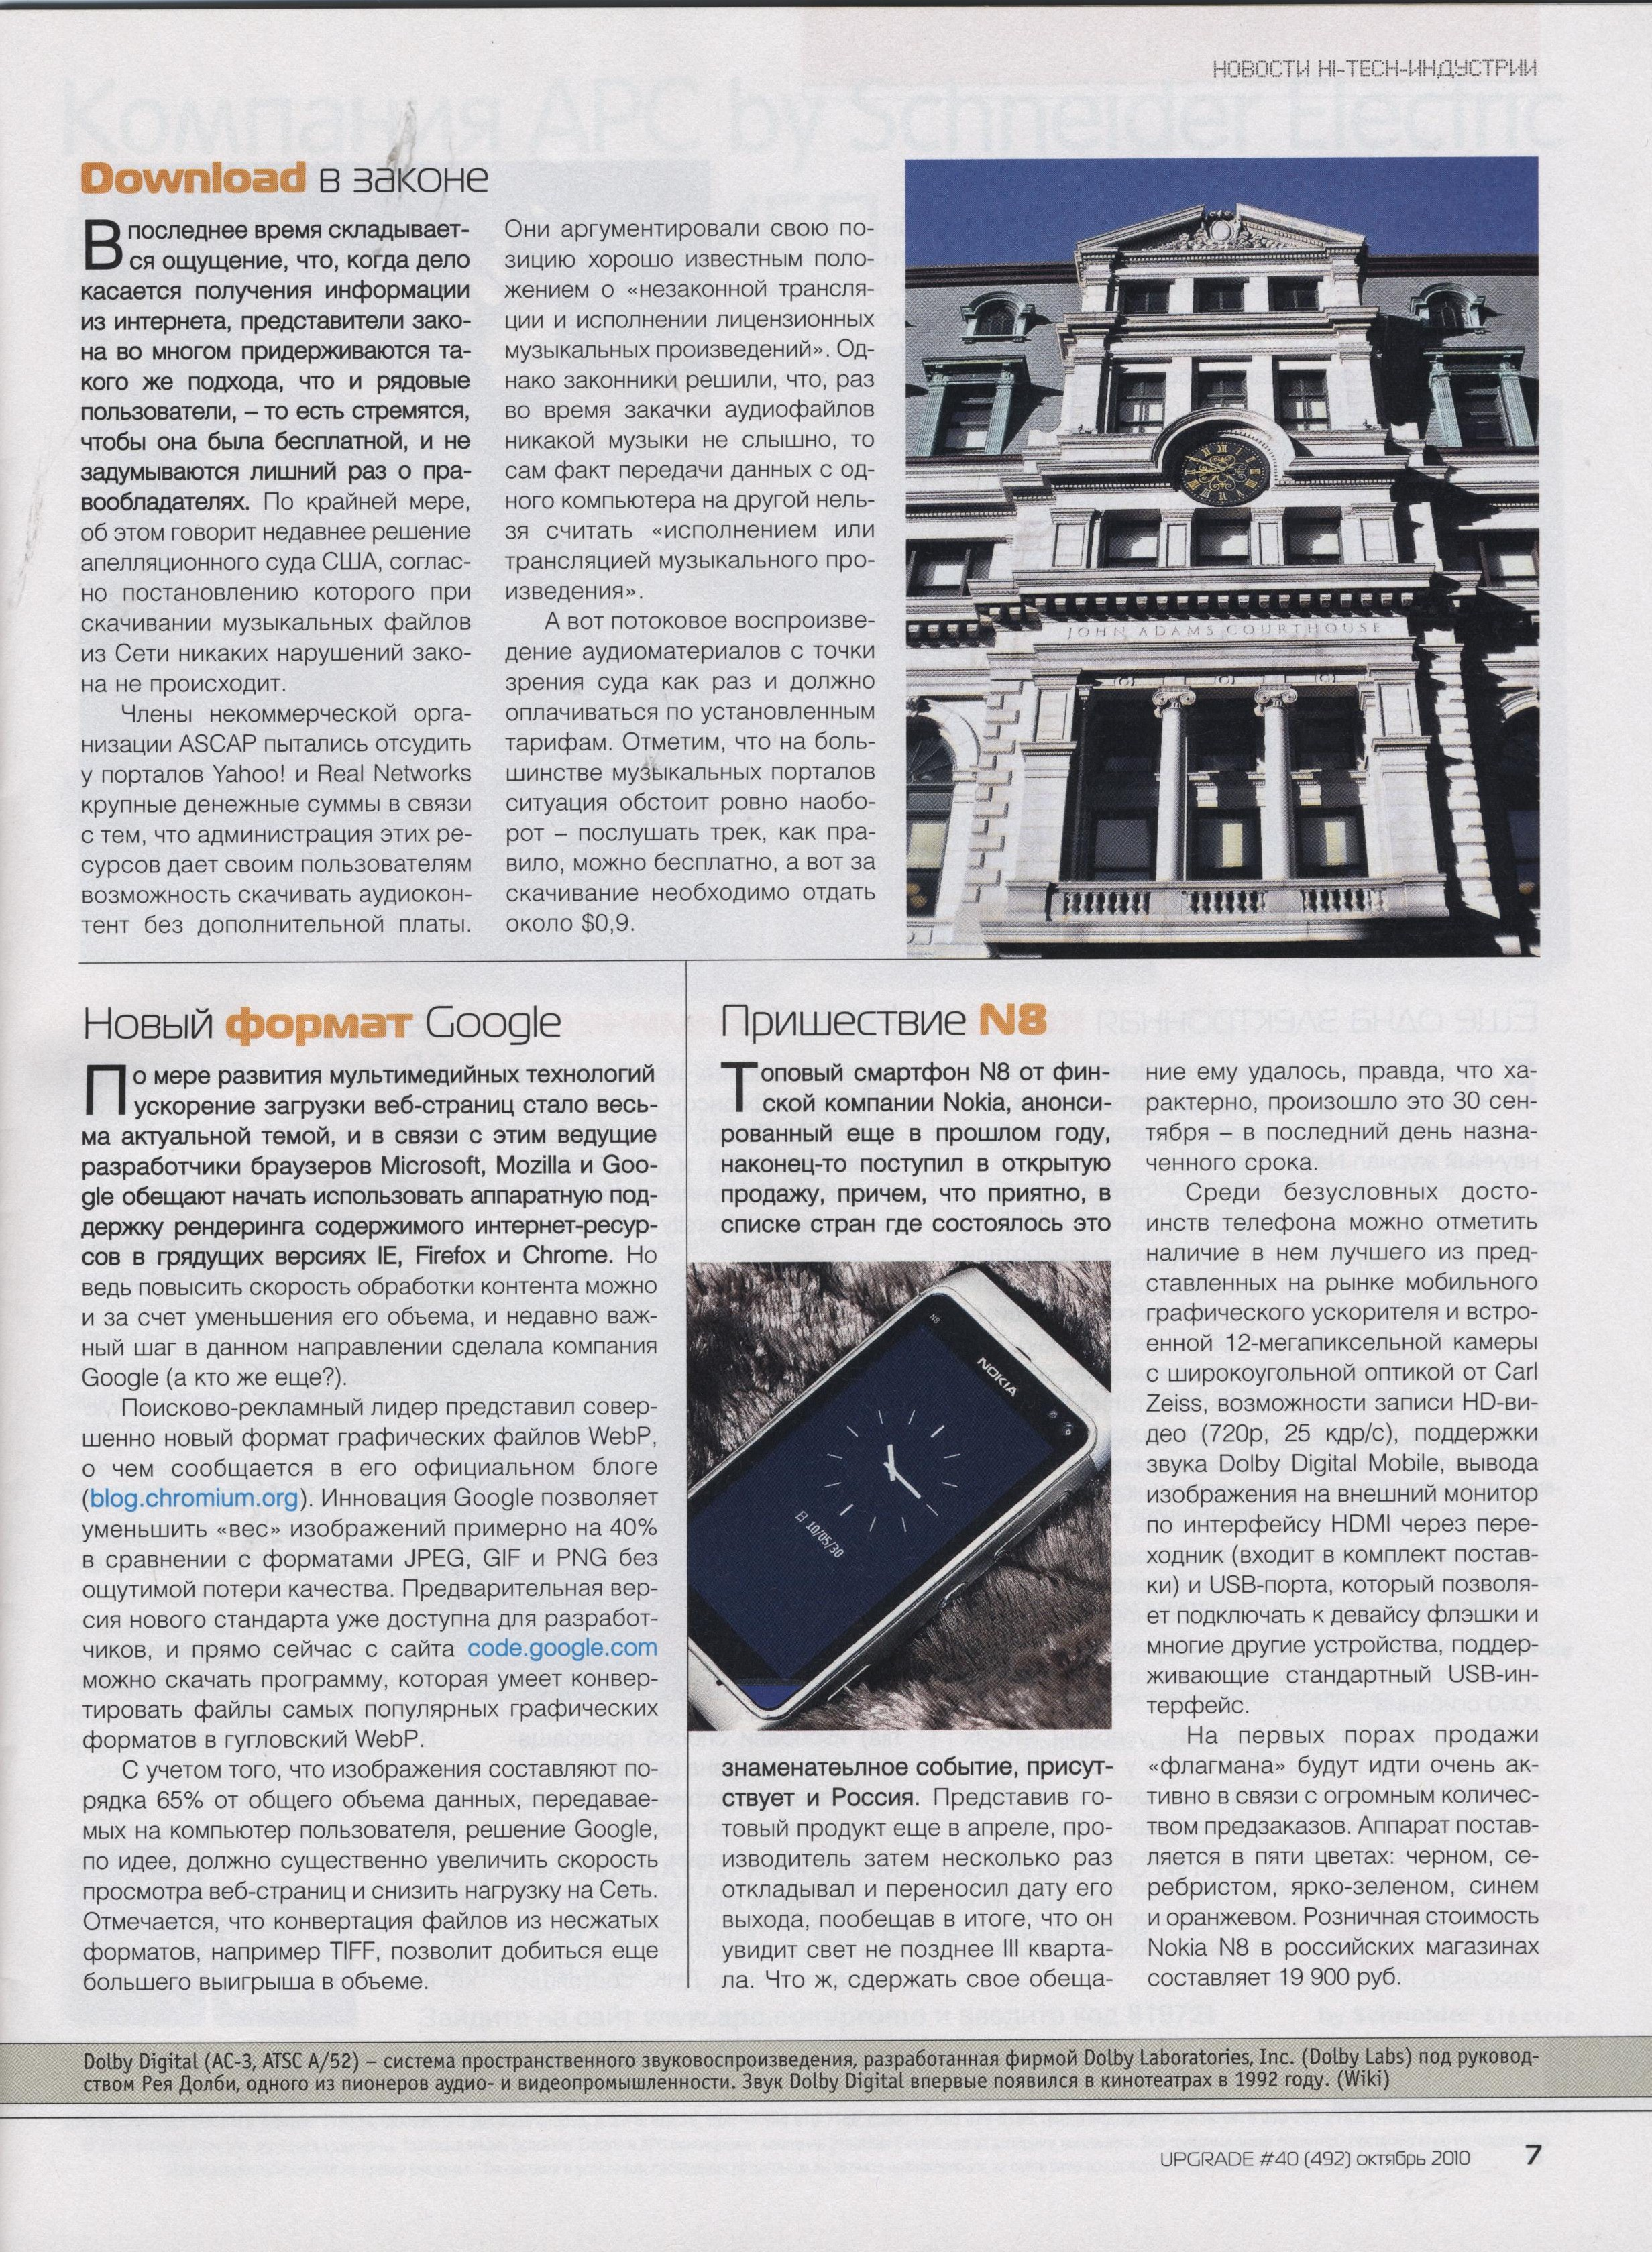
\includegraphics[scale=0.2]{images/4.jpg}
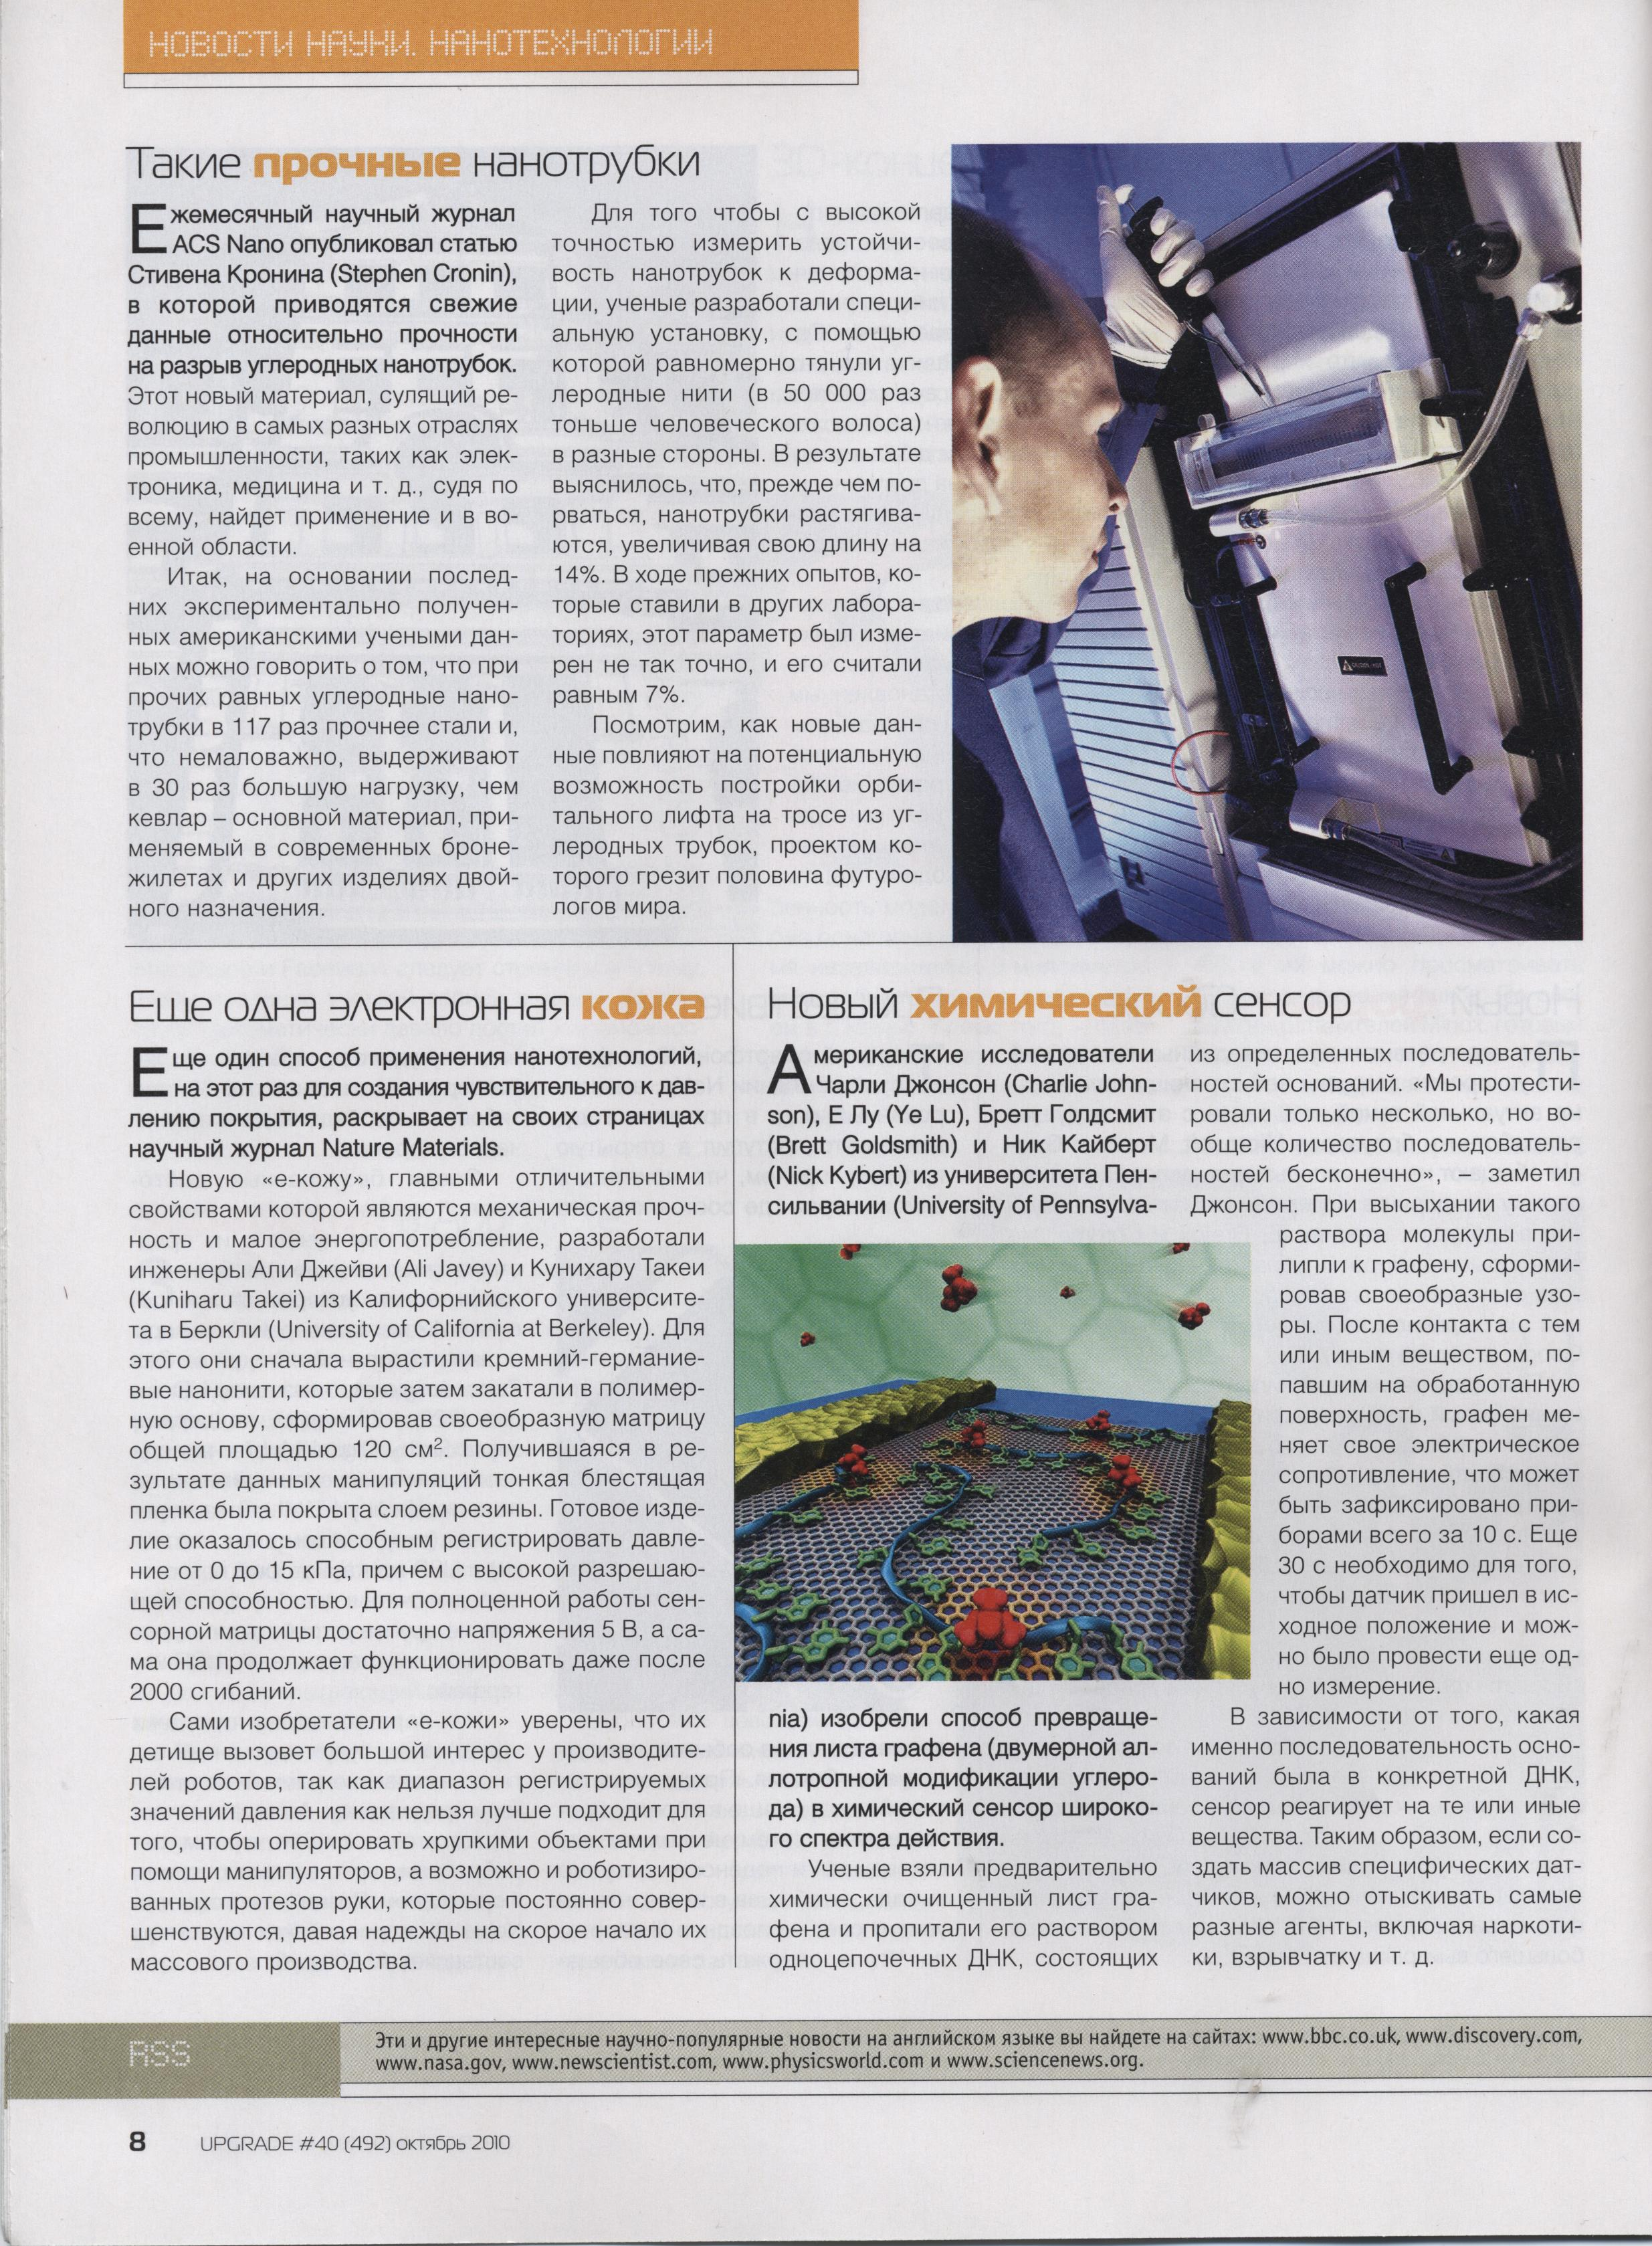
\includegraphics[scale=0.2]{images/5.jpg}
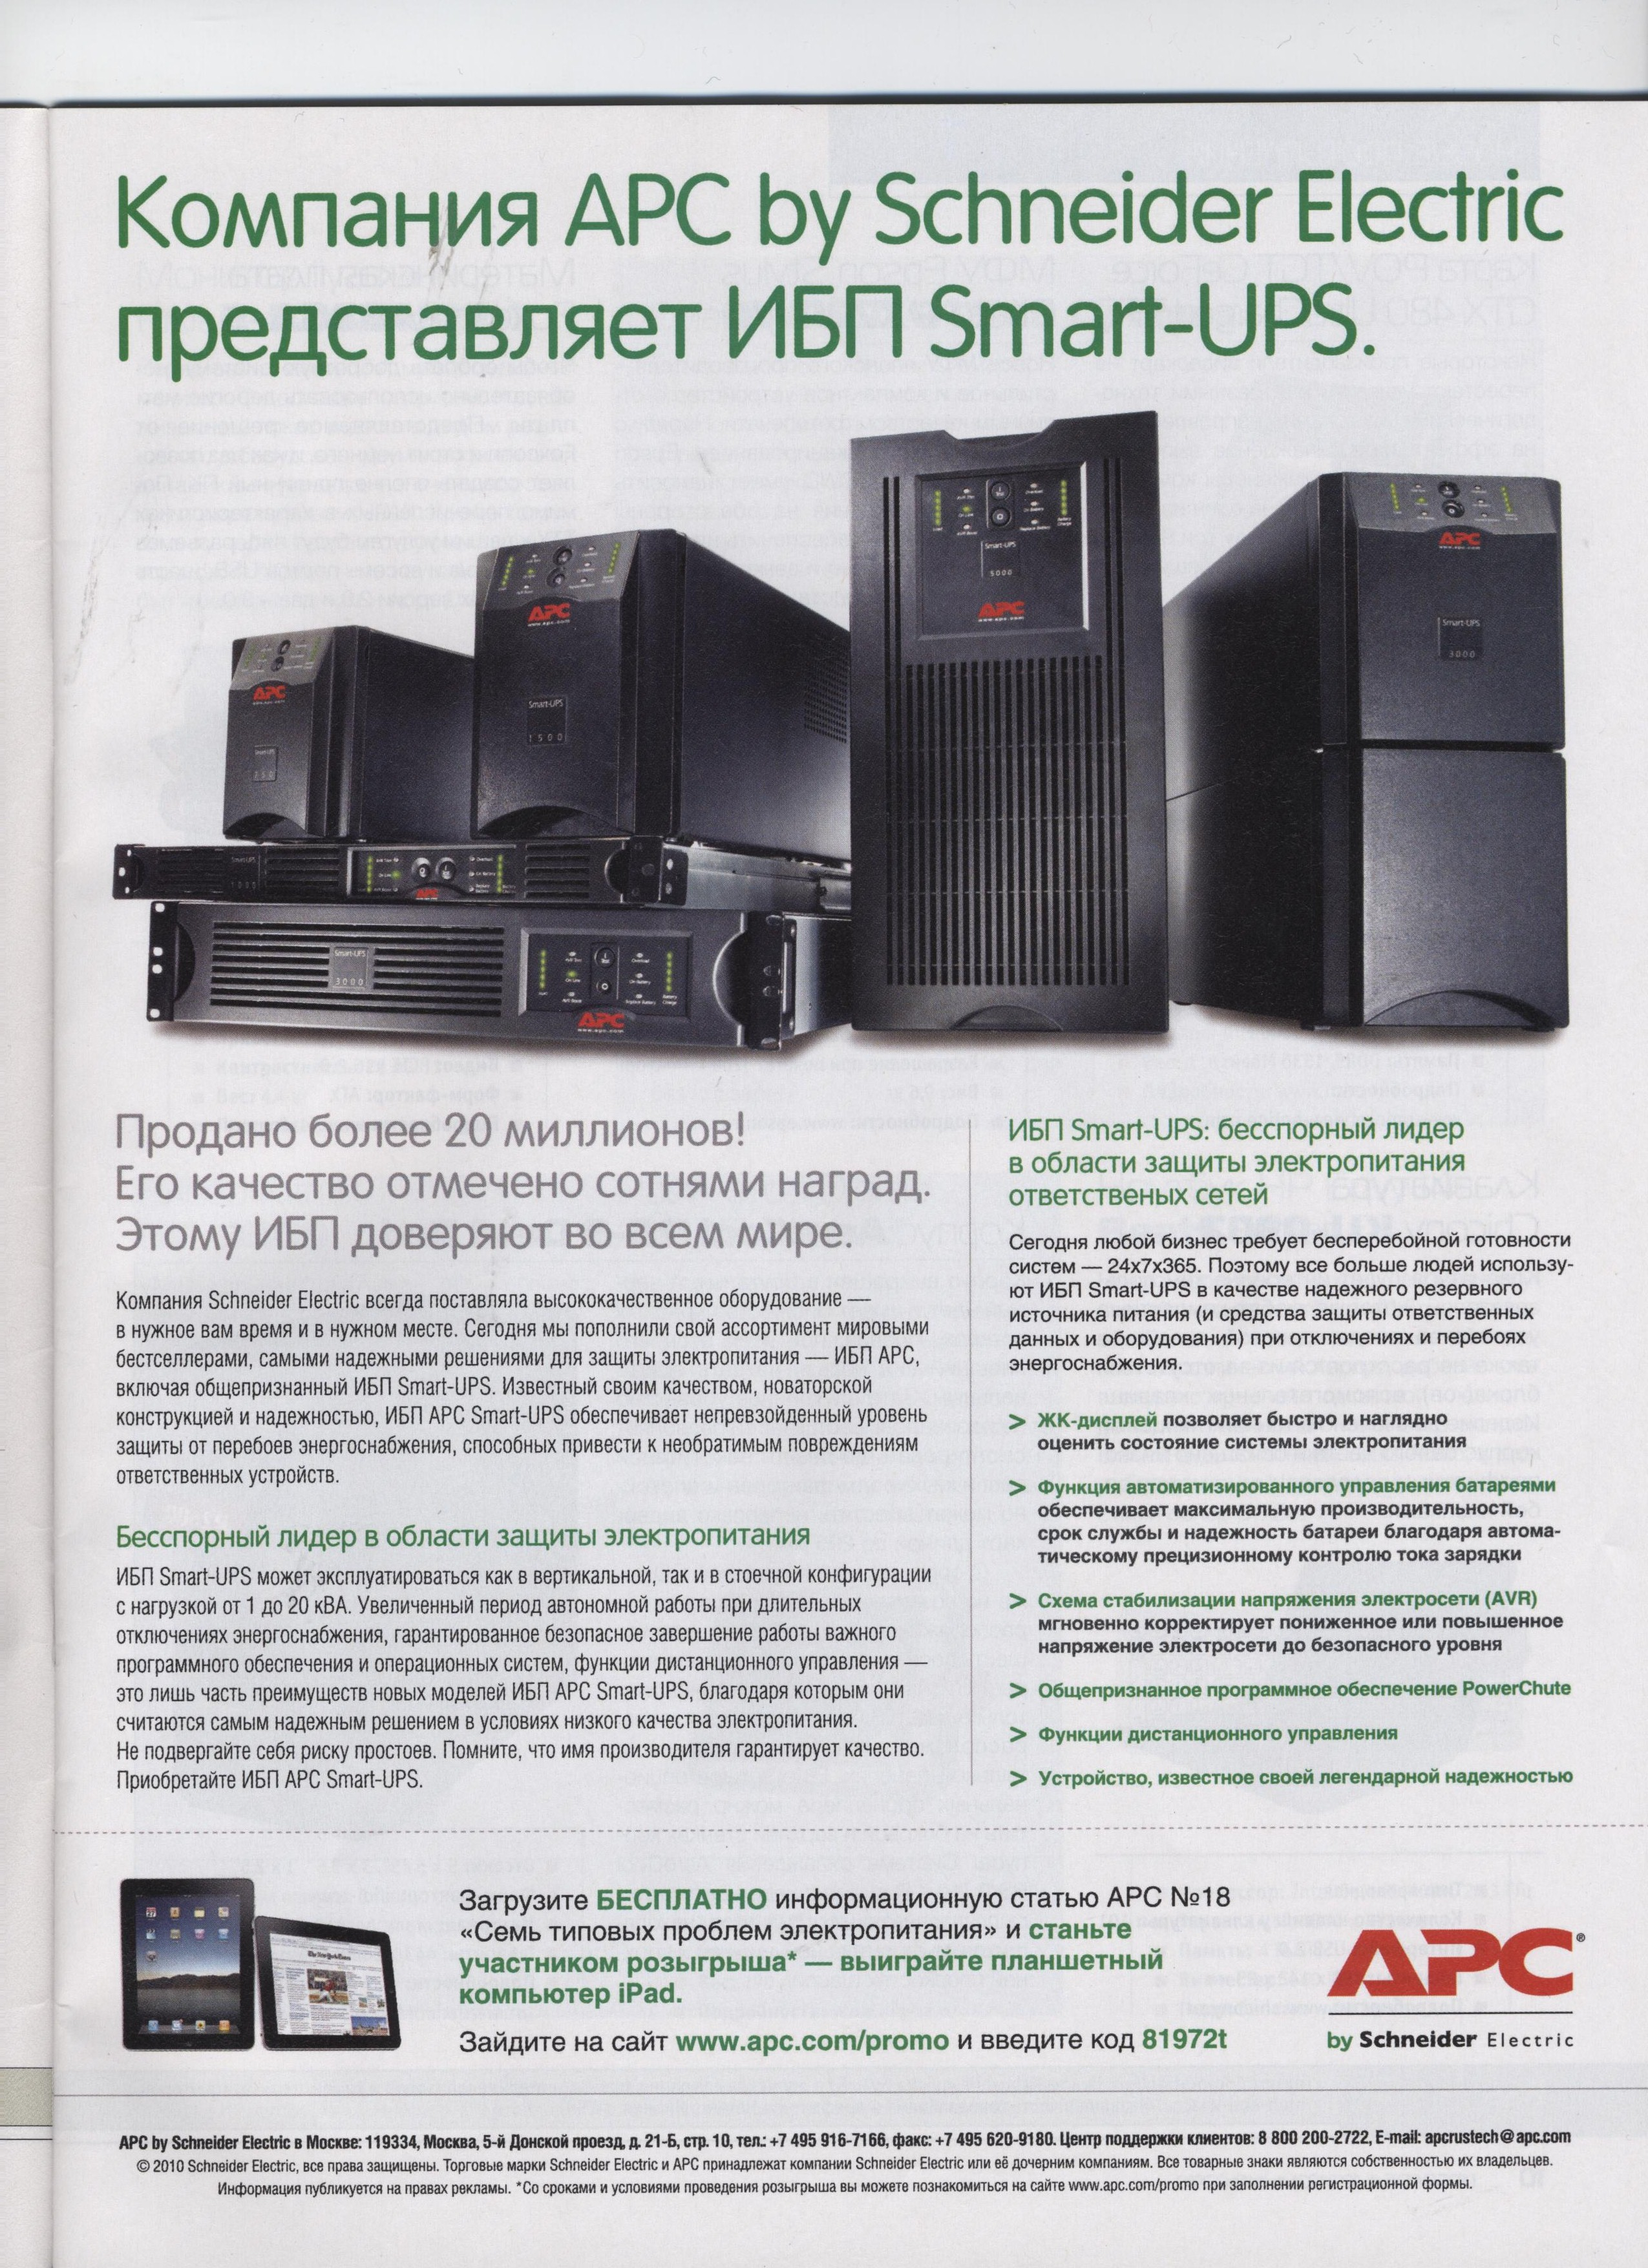
\includegraphics[scale=0.2]{images/6.jpg}
\end{center}
\caption{Exemples d'images du dataset}
\label{exemple}
\end{figure}
\clearpage

\section{Vérité-terrain}
A chacune de ces images est associée une image de vérite-terrain, attribuant à chaque pixel du document numérisé l'une des 3 classes parmi : \\
\begin{description} % listes descriptives

\item[$illustration$ :] Le pixel appartient à une illustration, une image, un fond d'image, un logo (en rouge sur les images vérité-terrain)
\item[$texte$ :] Le pixel appartient à un paragraphe de texte, un titre, un commentaire (en bleu sur les images vérité-terrain)
\item[$fond$ :] Le pixel appartient au fond blanc d'origine de la page (en blanc sur les images vérité-terrain).

\end{description}

Voici quelques exemples de documents numérisés et leur vérité terrain \ref{exemple1} \ref{exemple2} \ref{exemple3}.

\begin{figure}[H]
\begin{center}
\includegraphics[scale=0.2]{images/1g.jpg}
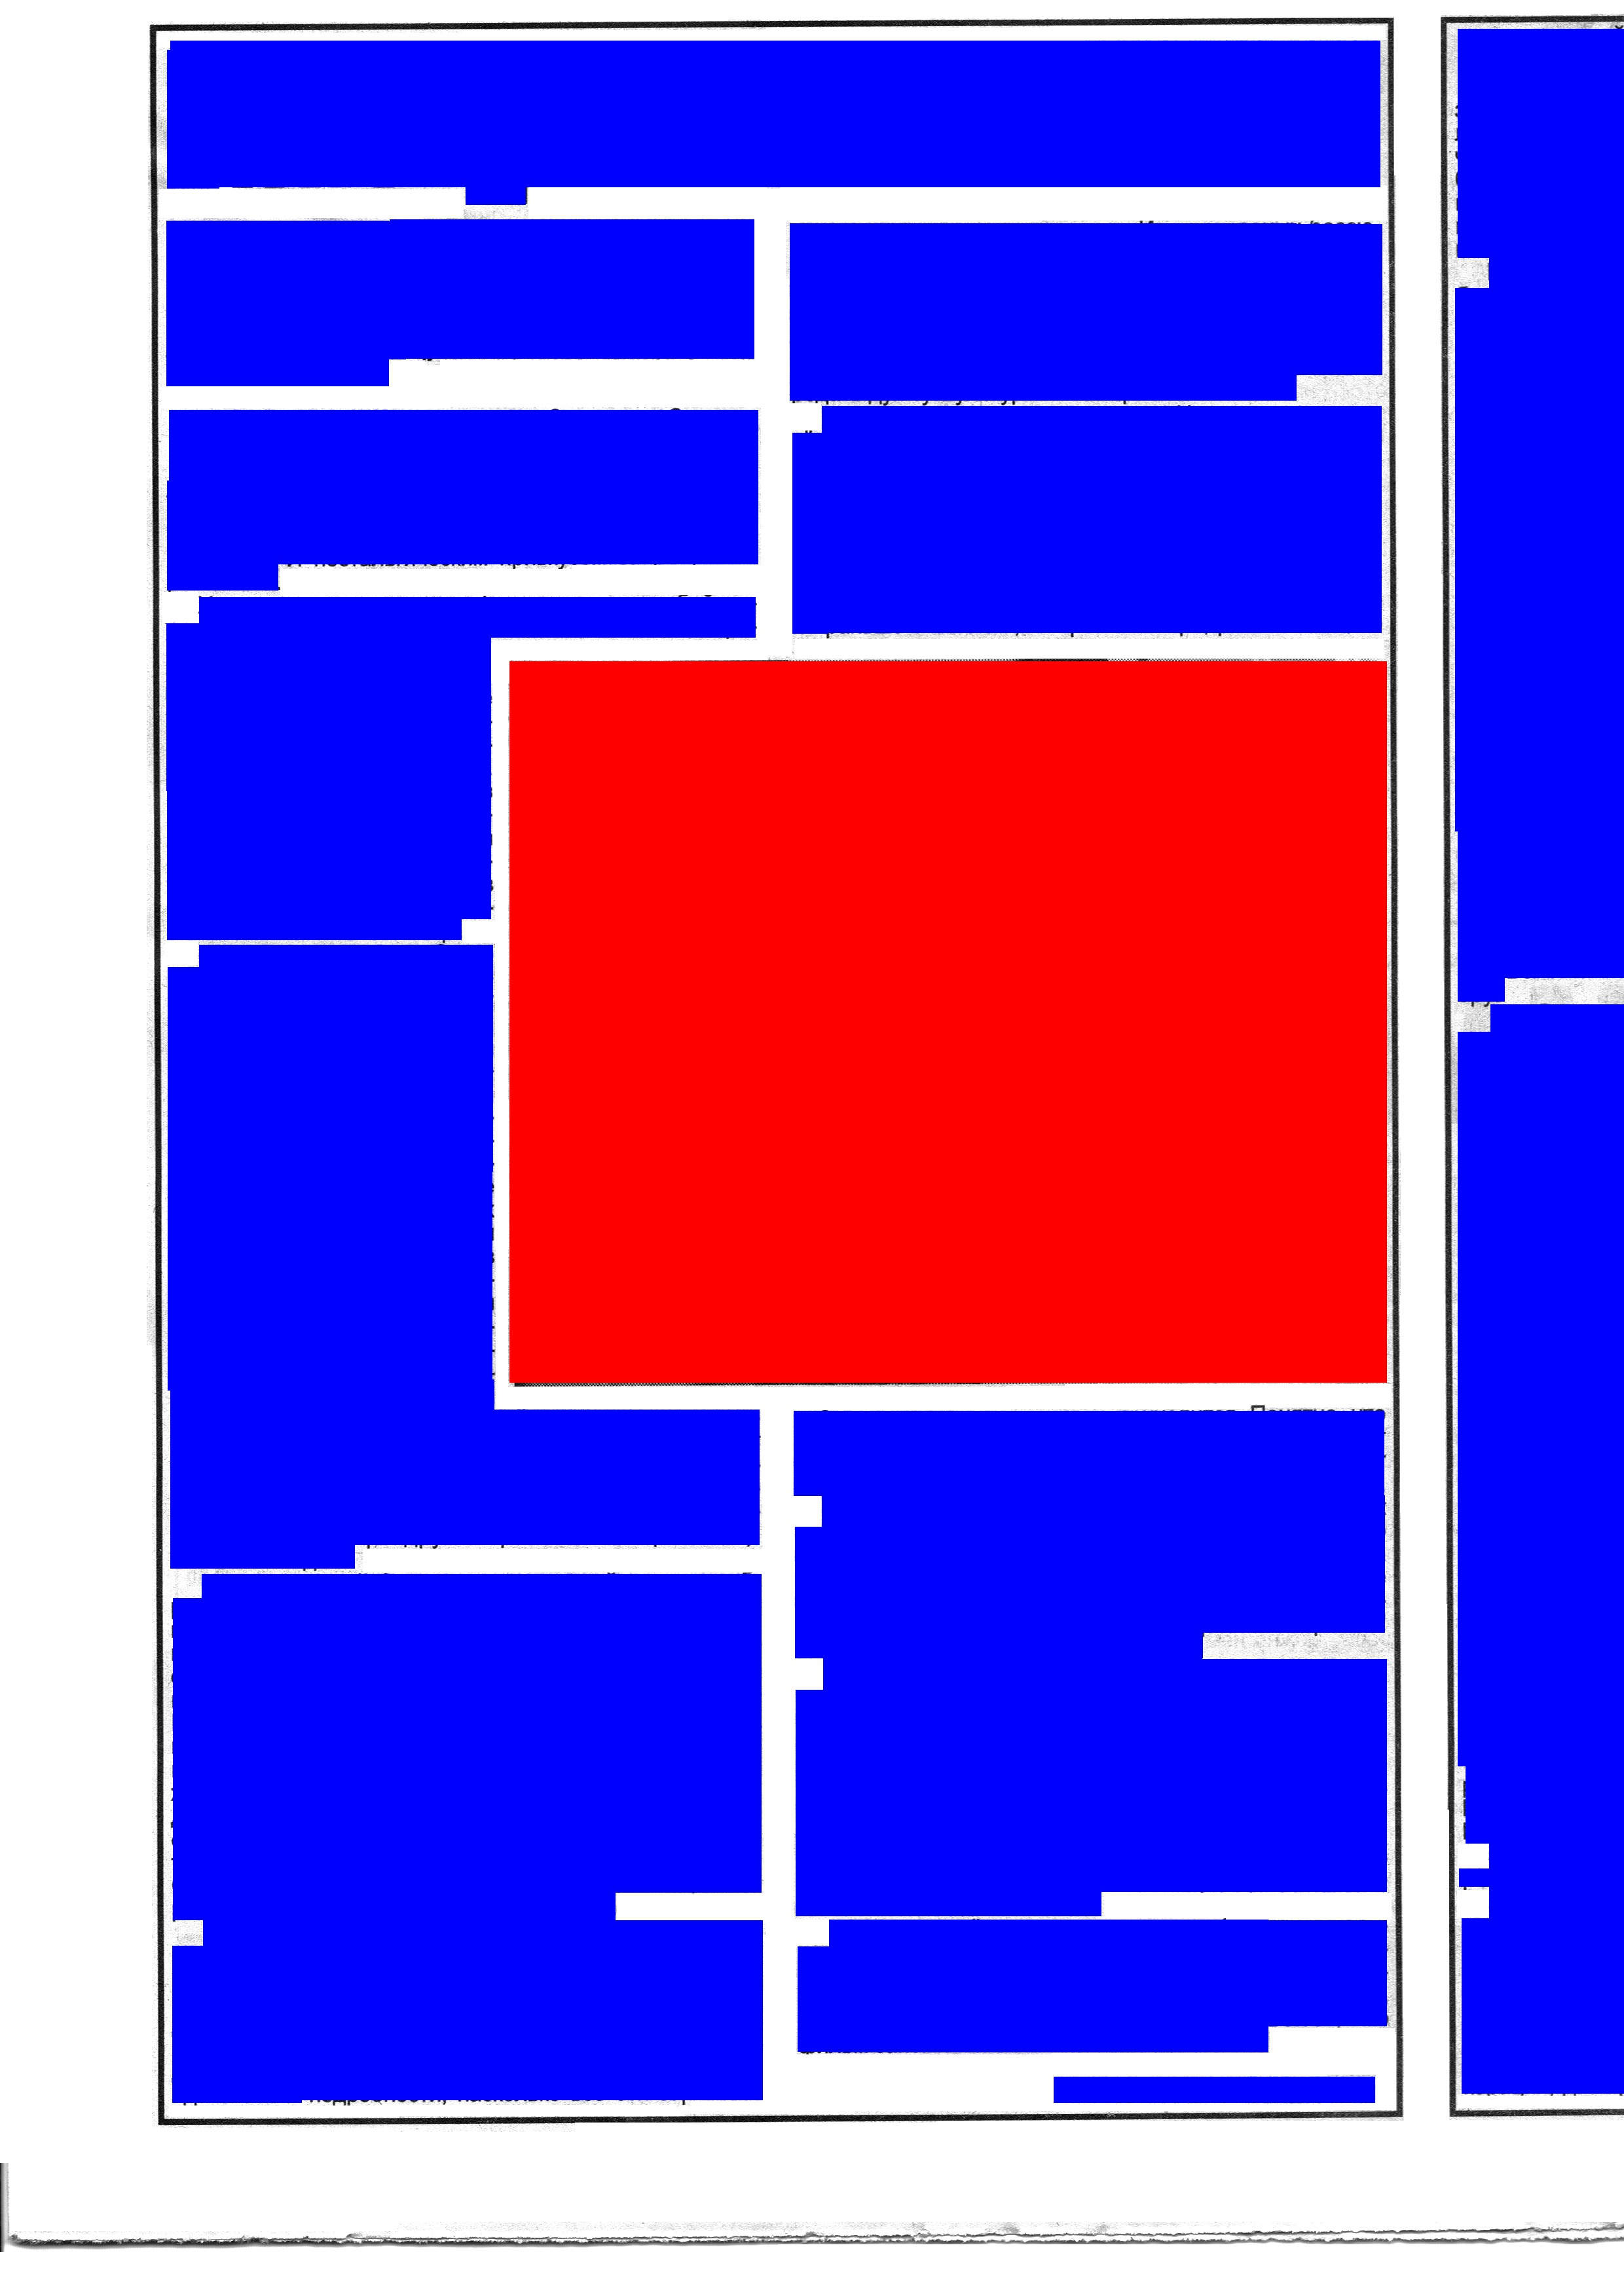
\includegraphics[scale=0.2]{images/1g_m.jpg}
\end{center}
\caption{image du dataset et sa vérité terrain}
\label{exemple1}
\end{figure}

\begin{figure}[H]
\begin{center}
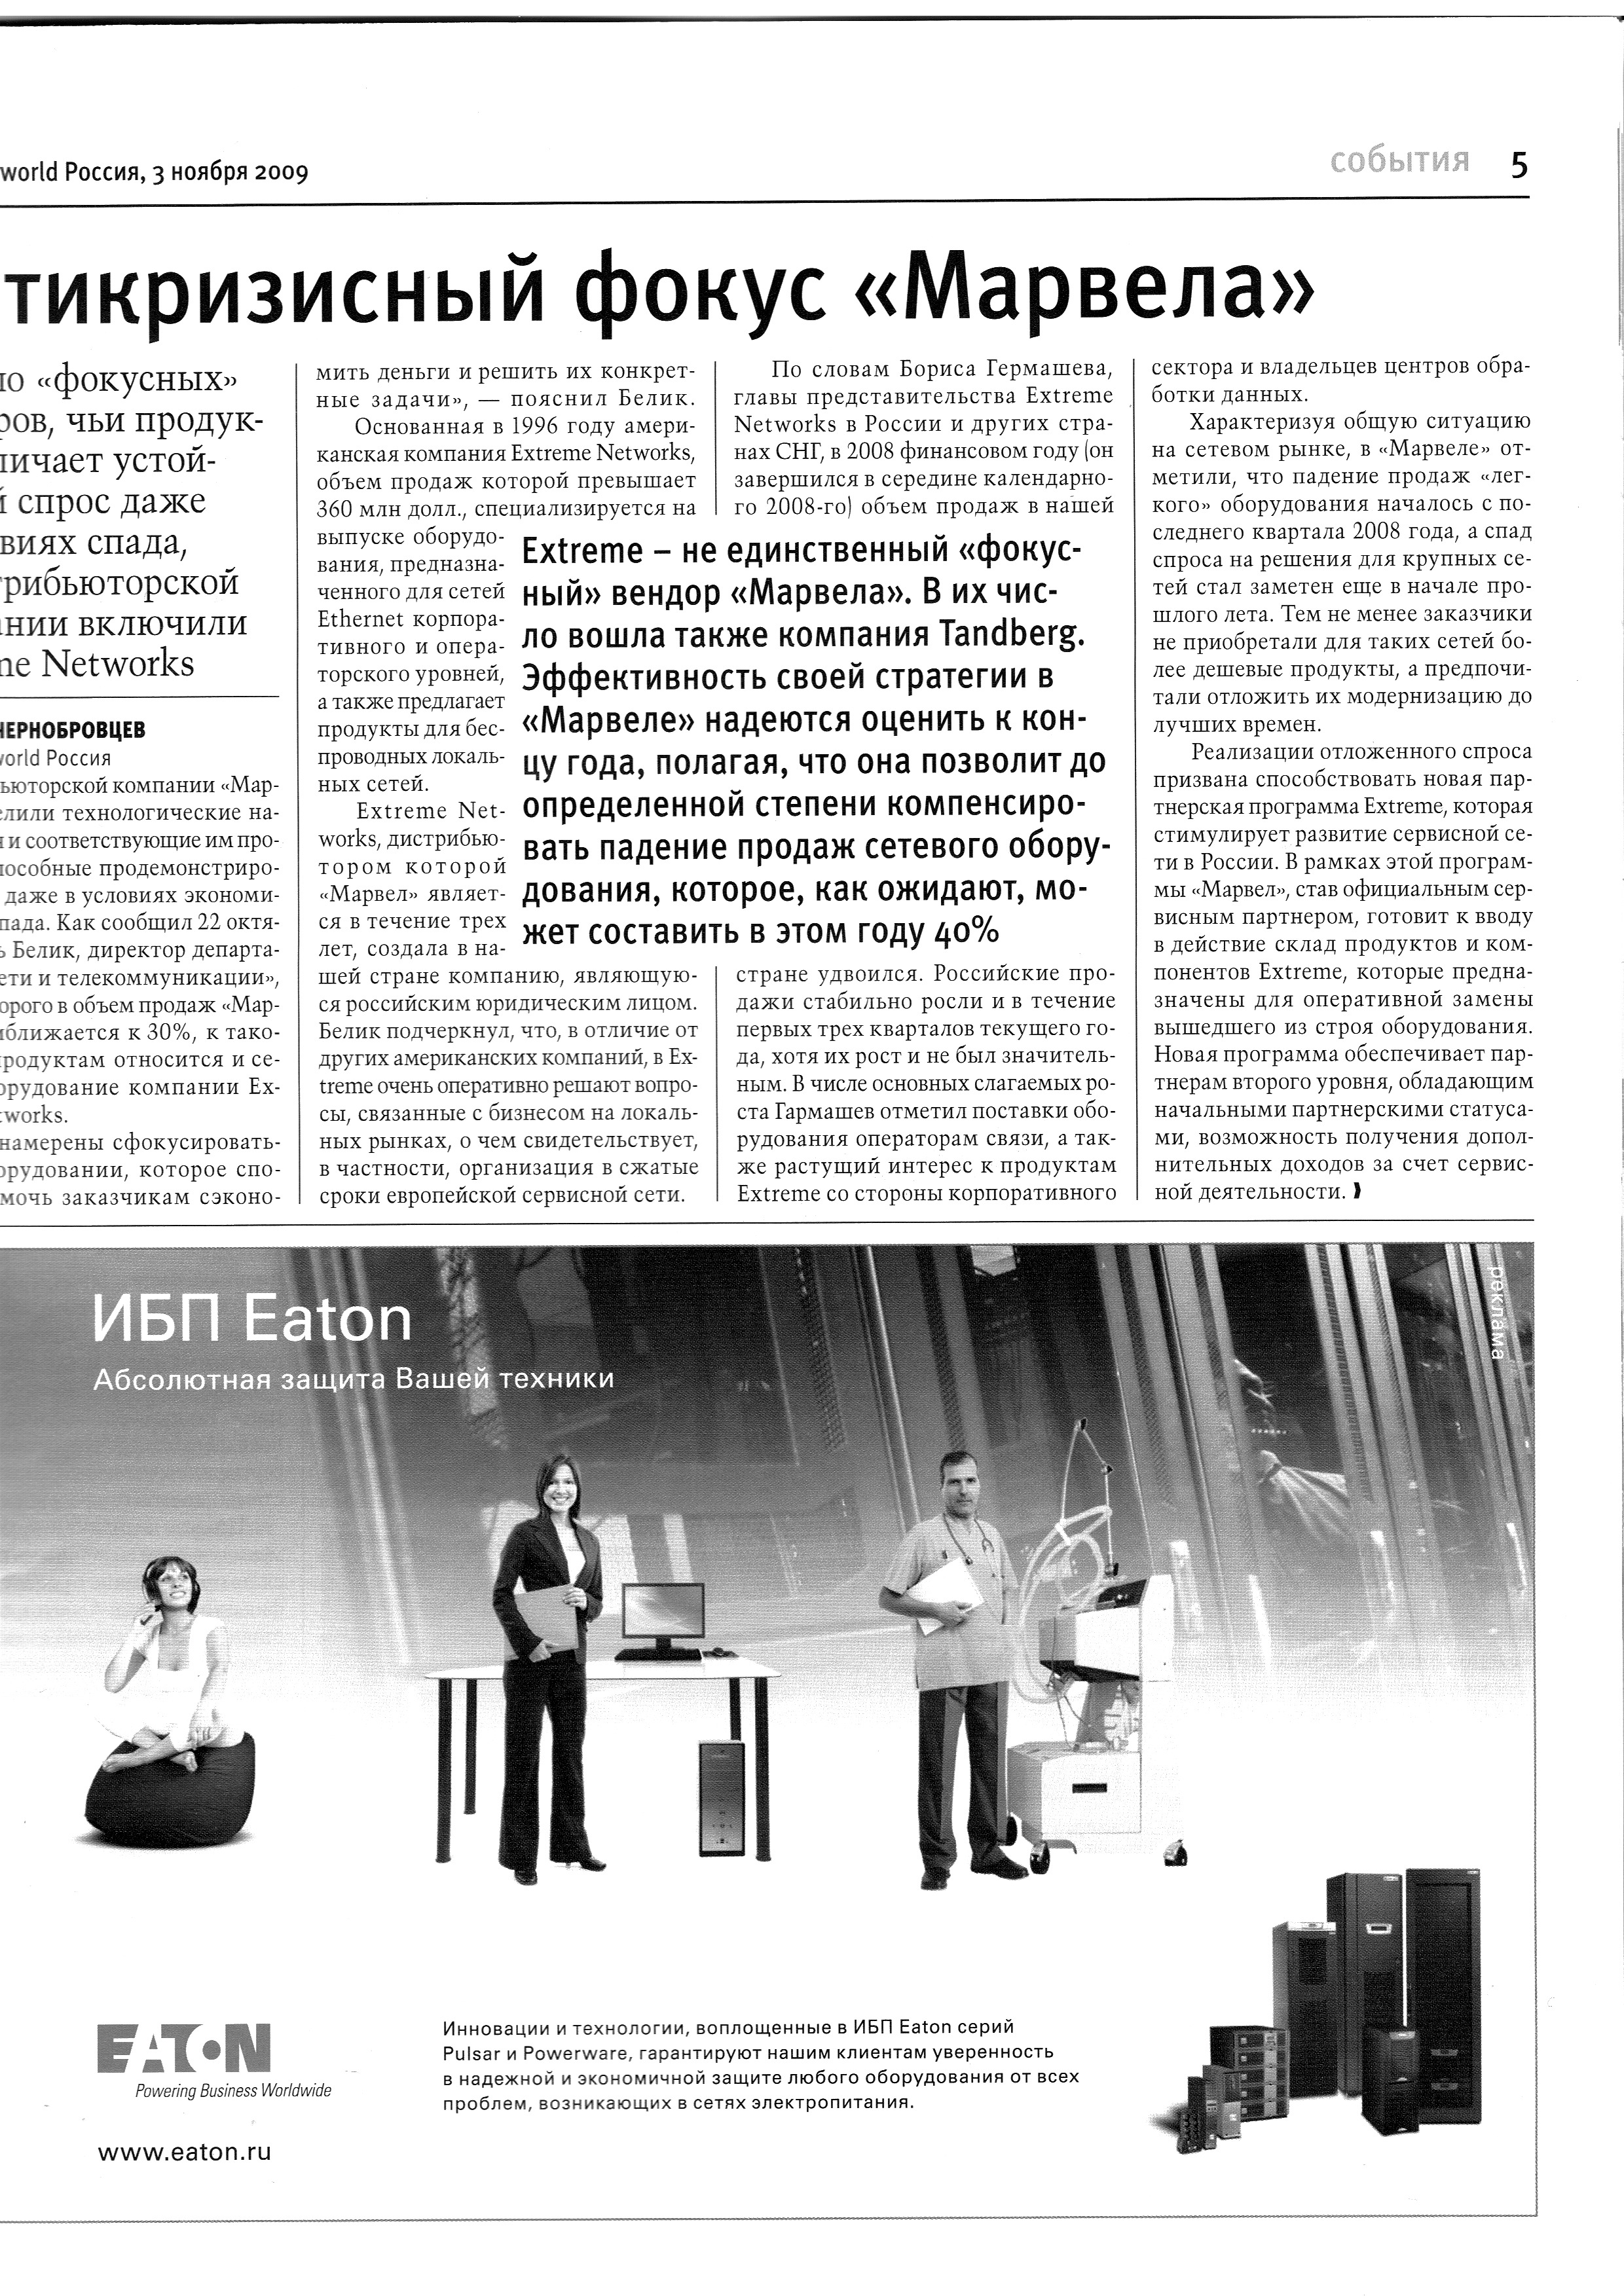
\includegraphics[scale=0.2]{images/4cw.jpg}
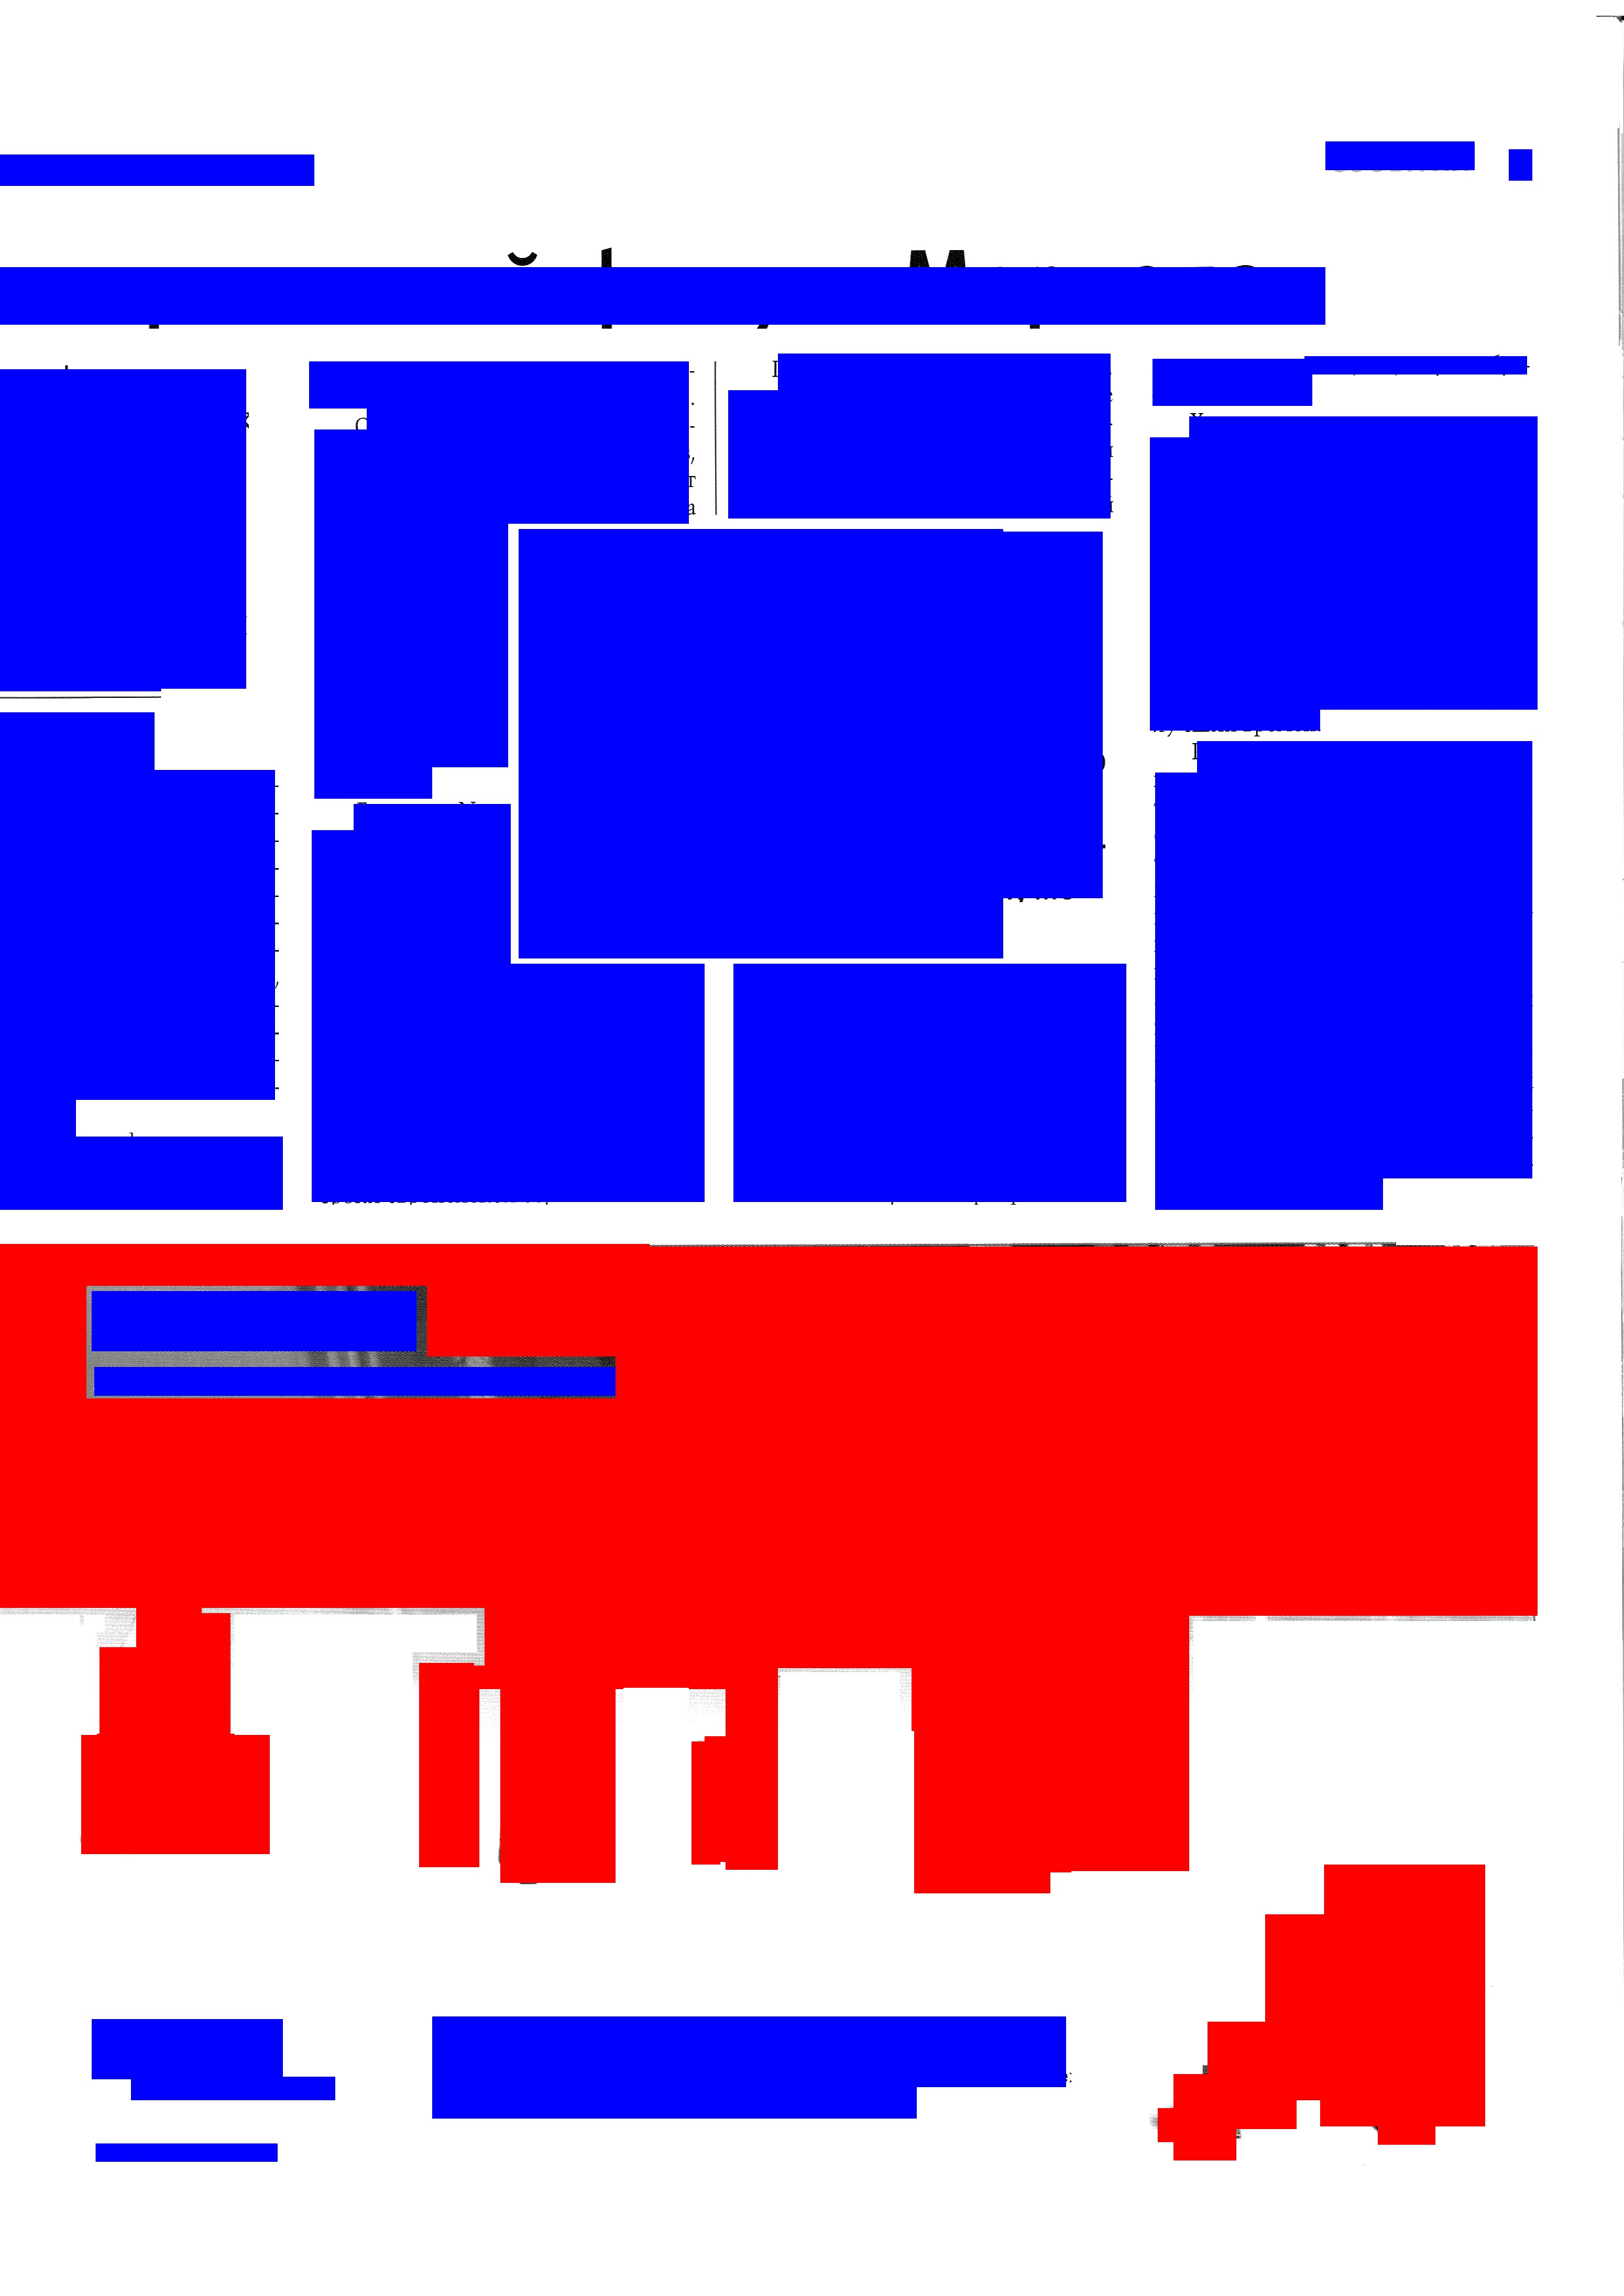
\includegraphics[scale=0.2]{images/4cw_m.jpg}
\end{center}
\caption{image du dataset et sa vérité terrain}
\label{exemple2}
\end{figure}

\begin{figure}[H]
\begin{center}

\includegraphics[scale=0.2]{images/56.jpg}

\includegraphics[scale=0.2]{images/56_m.jpg}
\end{center}
\caption{image du dataset et sa vérité terrain}
\label{exemple3}
\end{figure}
\clearpage

Par la suite, nous allons expliciter différentes manières d'extraire de l'information afin de pouvoir discriminer automatiquement, au sein d'une image, les pixels de classe
$illustration$, de classe $texte$ et de classe $fond$.

\chapter{Extraction d'information}
\section{Seuillage pour le fond}

Une manière simple et rapide d'isoler le fond, est de réaliser un seuillage de l'image passée en niveau de gris.\\
Le seuil d'Otsu cherche le seuil qui sépare l'histogramme des niveaux de gris en deux classes, de sorte que la variance inter-classe soit maximale, la variance intra-classe
minimale \ref{seuillage}.\\

\begin{figure}[H]
\begin{center}
\includegraphics[scale=0.3]{images/1g.jpg}
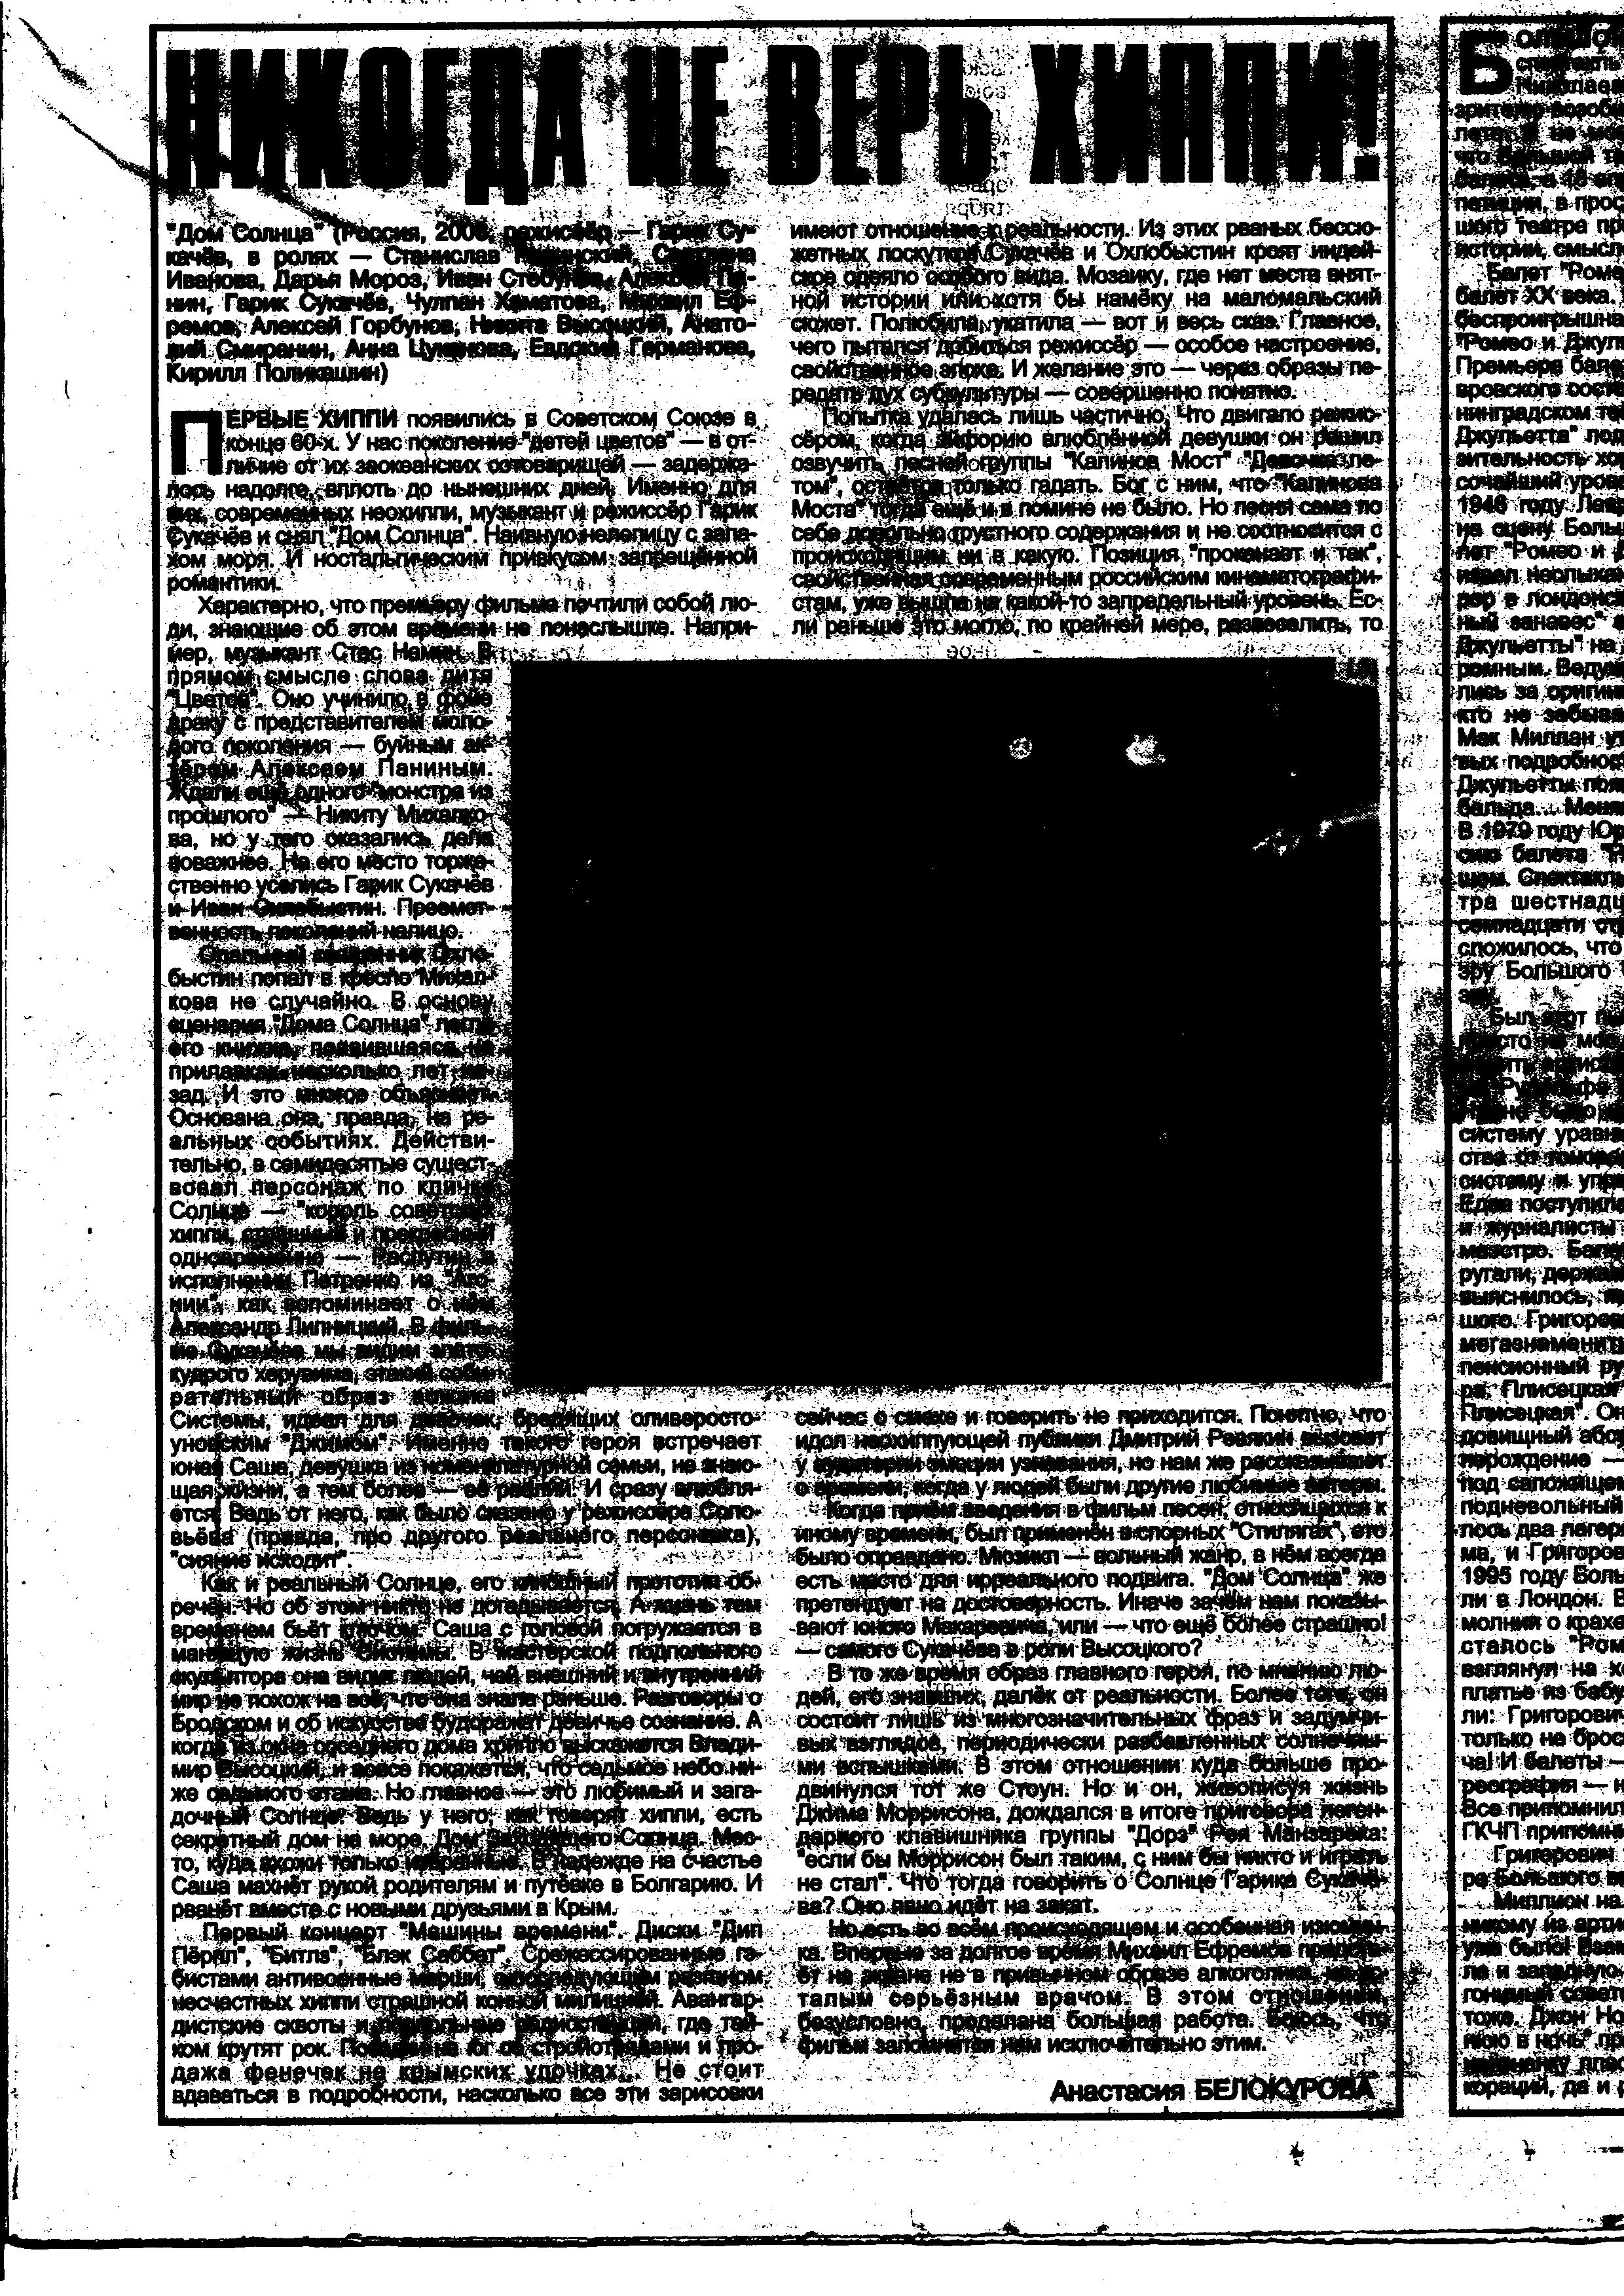
\includegraphics[scale=0.075]{images/1g_binary.jpg}
\end{center}
\caption{seuillage d'Otsu}
\label{seuillage}
\end{figure}

Ainsi, cette première étape permet de trouver les pixels de $fond$. En effet, on attribue une telle classe aux pixels dont le voisinage carré est à 95\% blanc 
dans l'image binaire \ref{classe_fond}

\begin{figure}[H]
\begin{center}
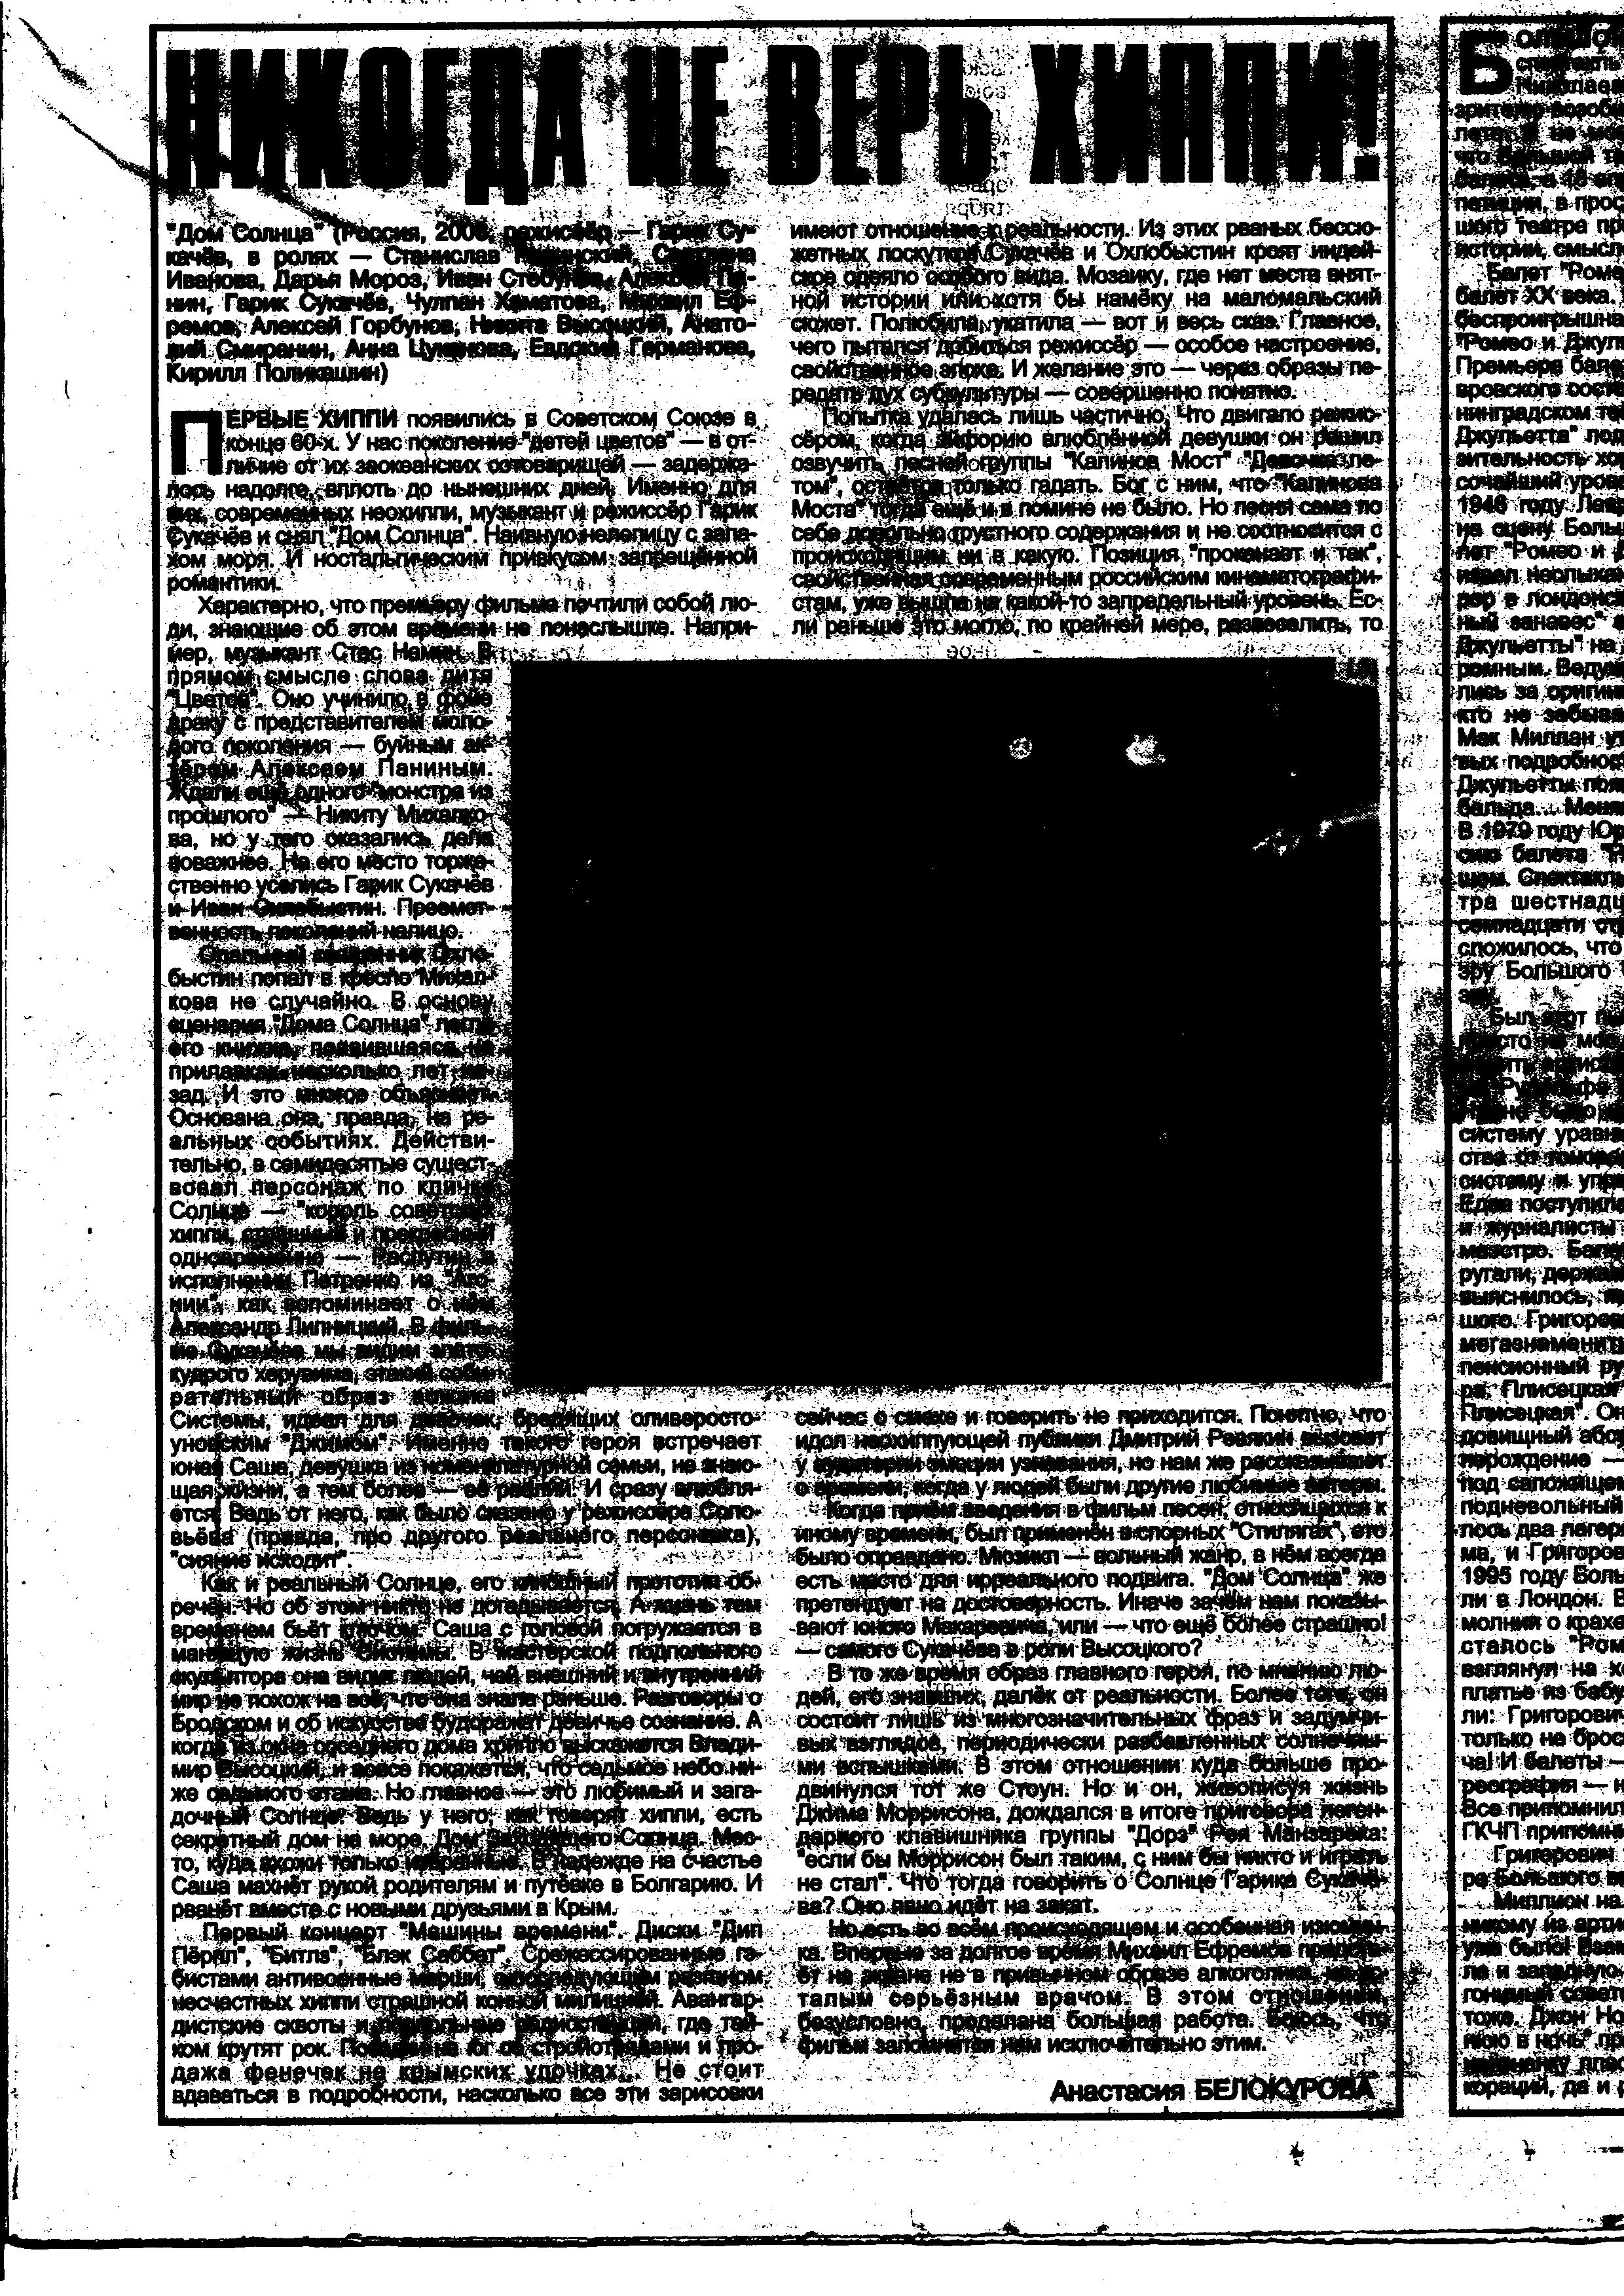
\includegraphics[scale=0.075]{images/1g_binary.jpg}
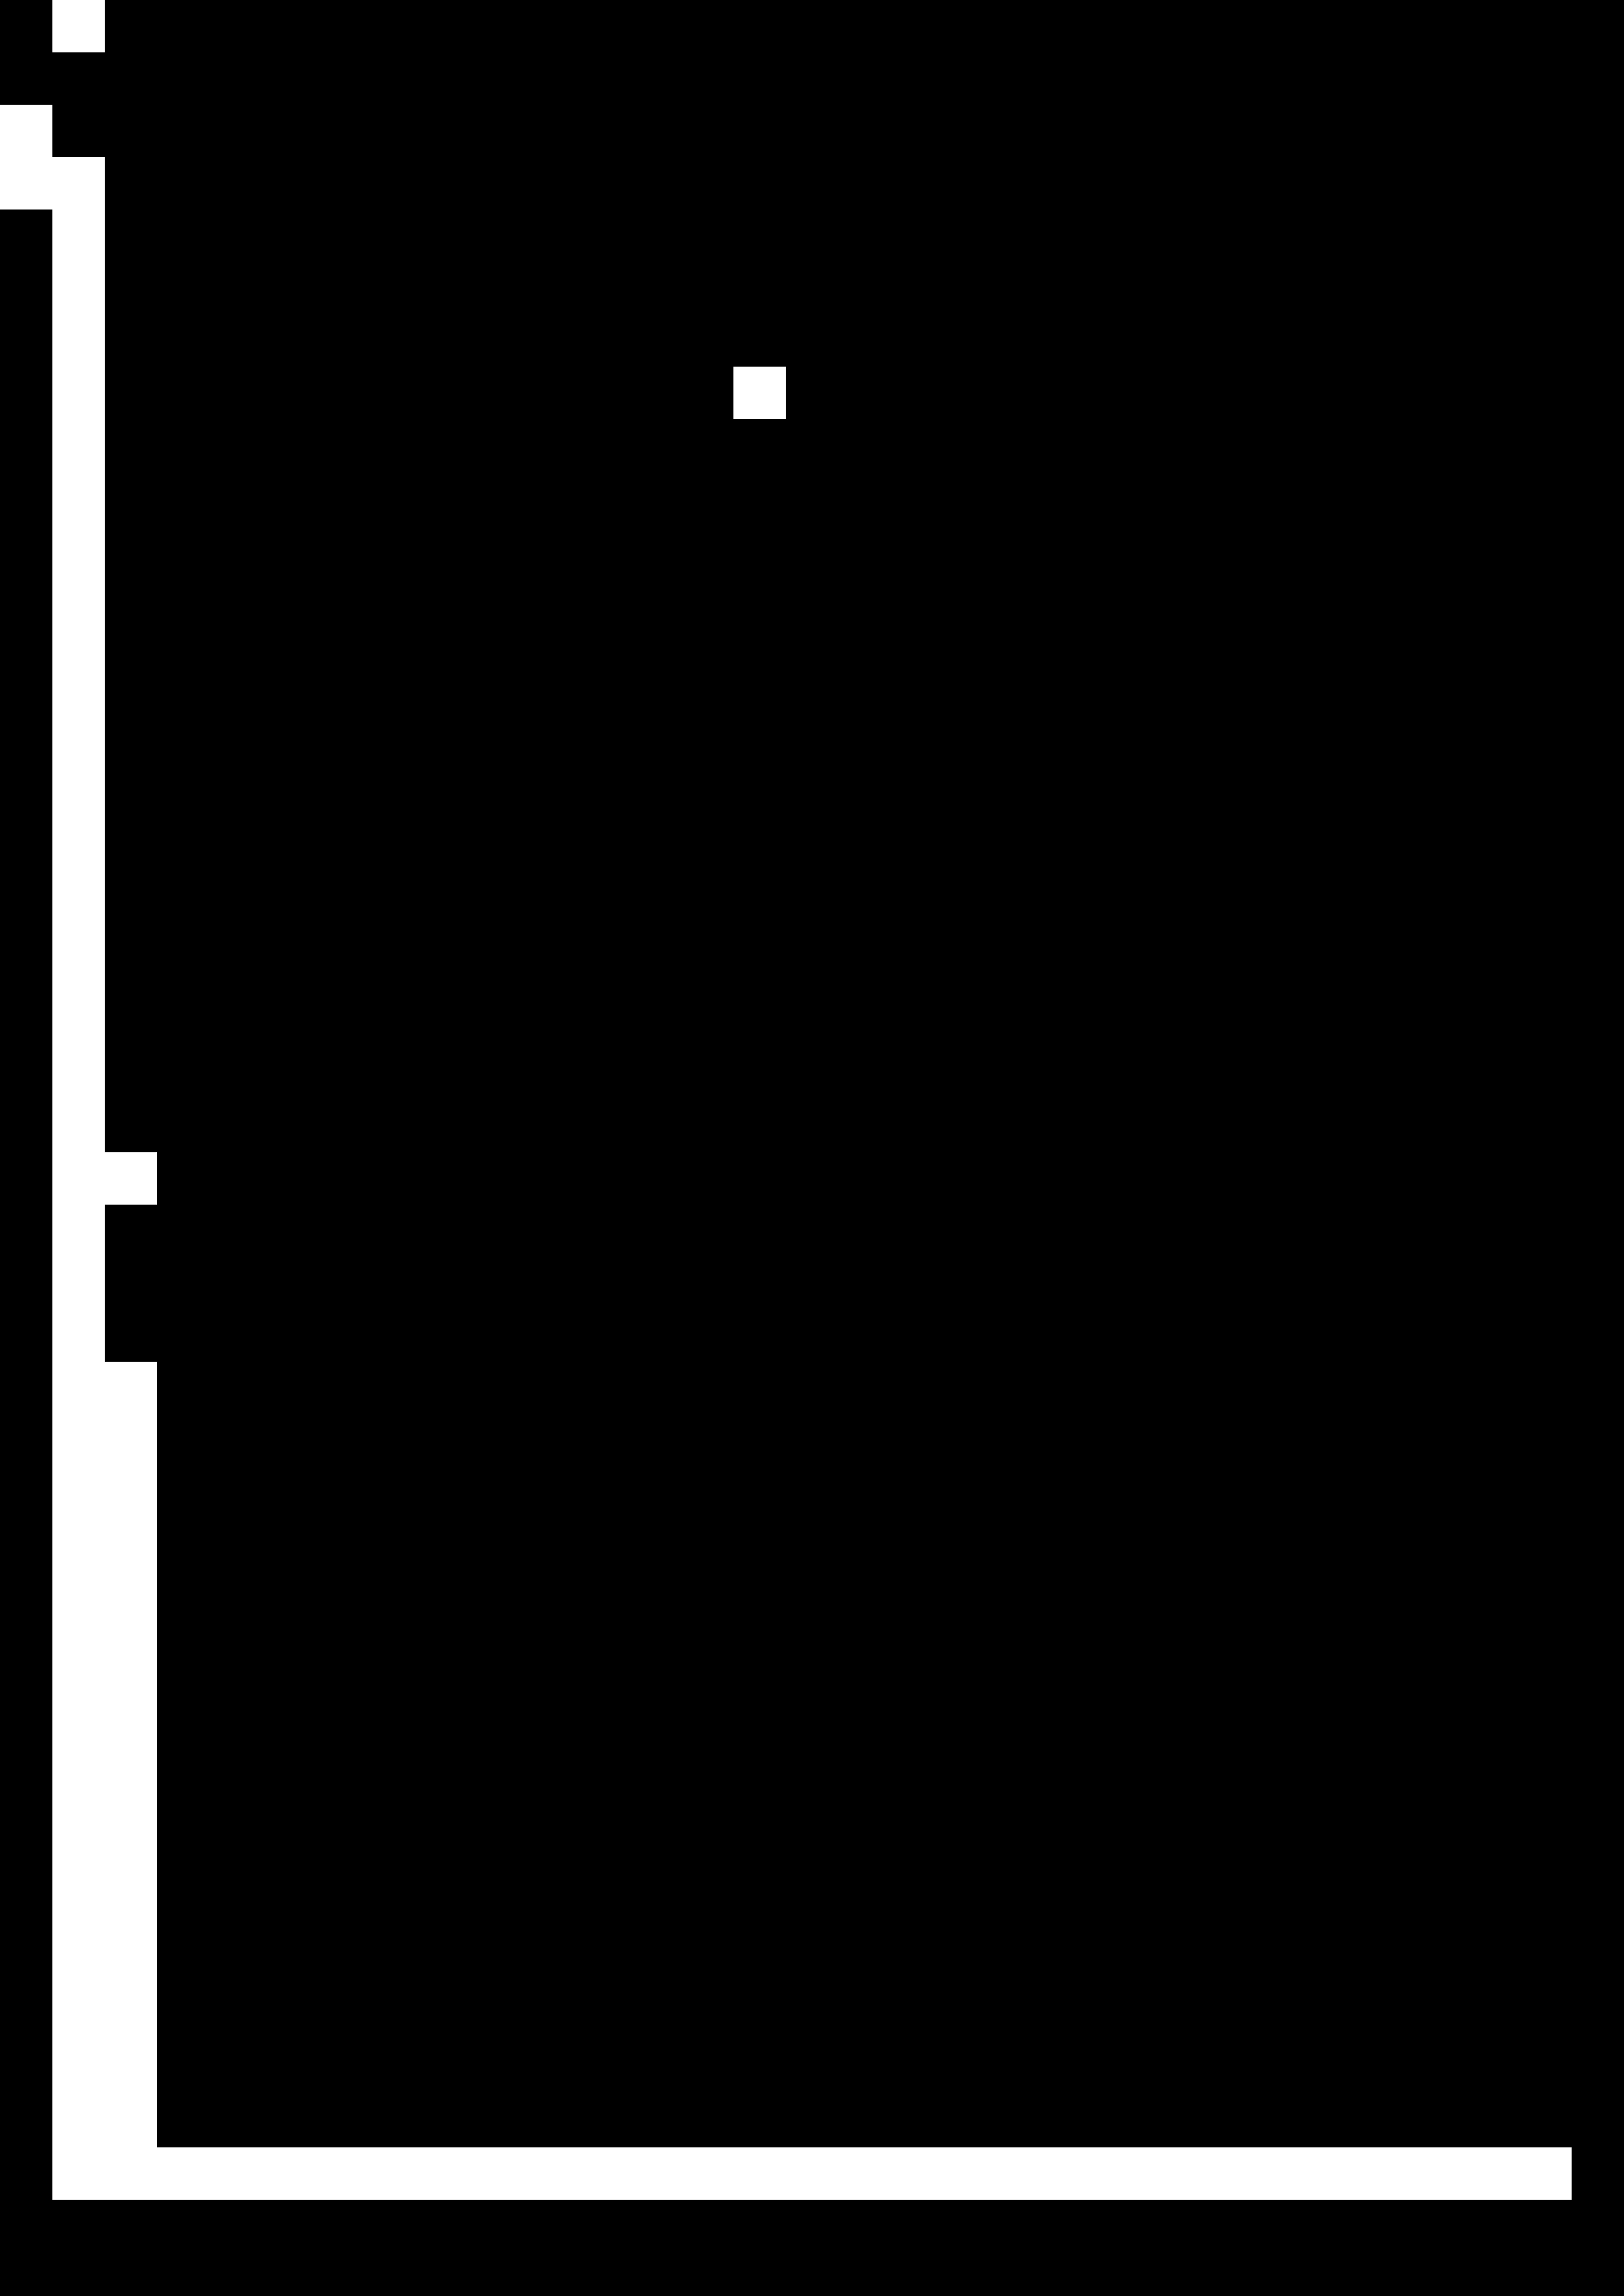
\includegraphics[scale=0.075]{images/1g_seuil.jpg}
\end{center}
\caption{seuillage puis attribution de la classe $fond$ (voisinage de taille 40 pixels)}
\label{classe_fond}
\end{figure}

Reste à definir une classe ($texte$ ou $illustration$) aux pixels restants.

\section{Extraction de contours pour le texte}

Les contours au voisinage d'un pixel, semblent être une information pertinente pour caractériser les caractères d'un document numérisé.\\
En effet, les caractères sont généralement d'une couleur uniforme sur un fond uniforme (pour plus de lisiblité), ce qui a la 
particularité de bien faire ressortir les gradients\\
Pour extraire cette information, deux méthodes seront utilisées : ou bien l'application d'un filtre Laplacien, ou bien le calcul de l'histogramme orienté du gradient 
\cite{Dalal05histogramsof}, cela sur un patch carré centré autour de chaque pixel. 

\section{Extraction de saturation pour les illustrations}

Comme évoqué precedemment, l'extraction d'une caractéristique de couleur est utile pour isoler les pixels d'illustration.\\
Cependant, utiliser les triplets RGB au voisinage d'un pixel n'a que peu de sens si on cherche à discriminer des pixels de texte (souvent noir).
En effet, le triplet HSV est plus approprié dans ce contexte : la saturation en particulier pour différencier les images couleur du texte gris-noir.\\
Les histogrammes des figures \ref{histo_hsv_illustration} et \ref{histo_hsv_texte} montrent parfaitement cette propriété : les patchs de texte ont des saturations
proches de 0, contrairement aux patchs d'illustration.\\

\begin{figure}[H]
\begin{center}
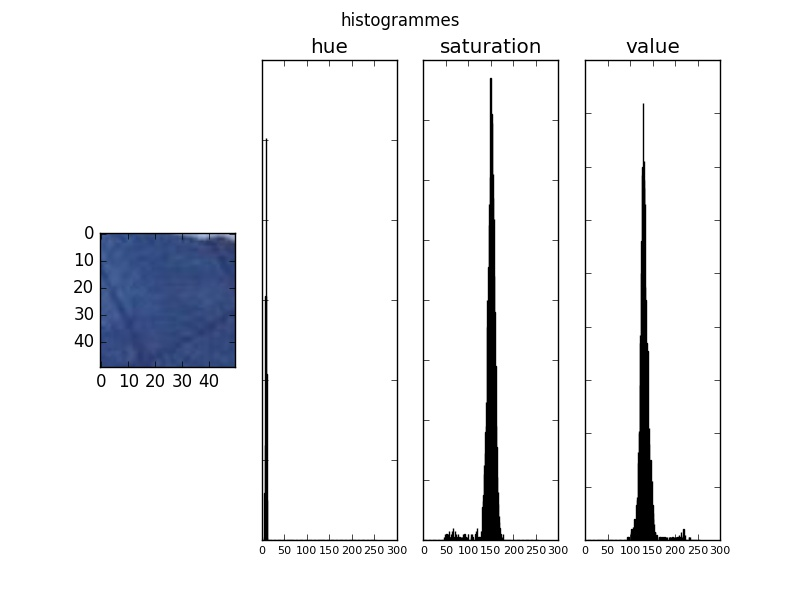
\includegraphics[scale=0.3]{images/histo_hsv_image.jpg}
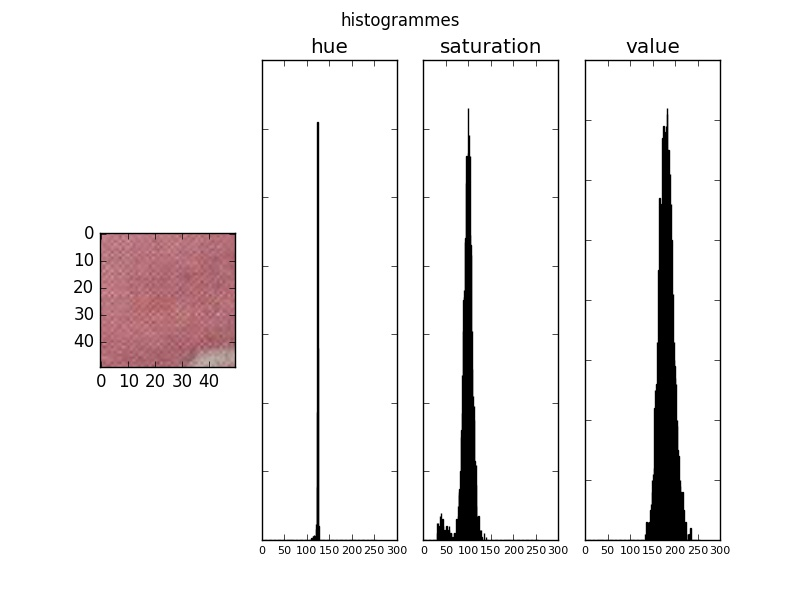
\includegraphics[scale=0.3]{images/histo_hsv_image2.jpg}
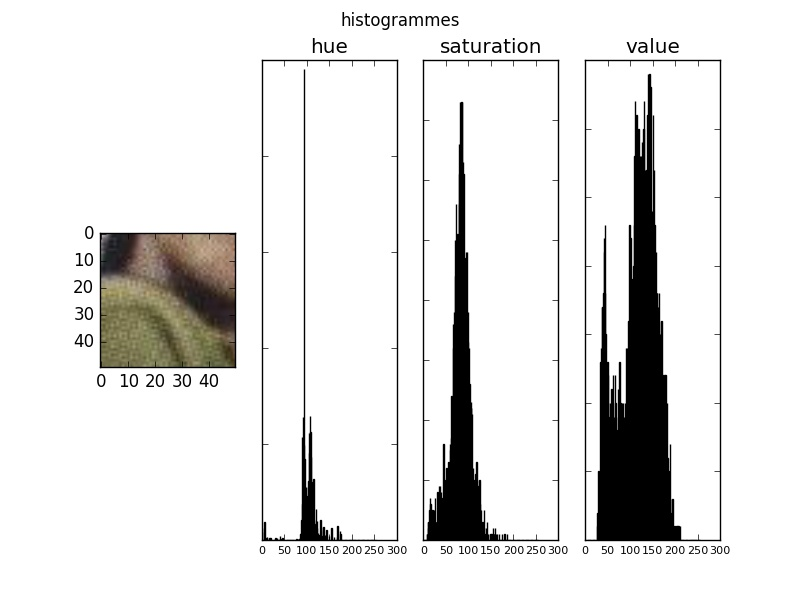
\includegraphics[scale=0.3]{images/histo_hsv_image3.jpg}
\end{center}
\caption{histogrammes HSV pour trois patchs d'illustration}
\label{histo_hsv_illustration}
\end{figure}

\begin{figure}[H]
\begin{center}
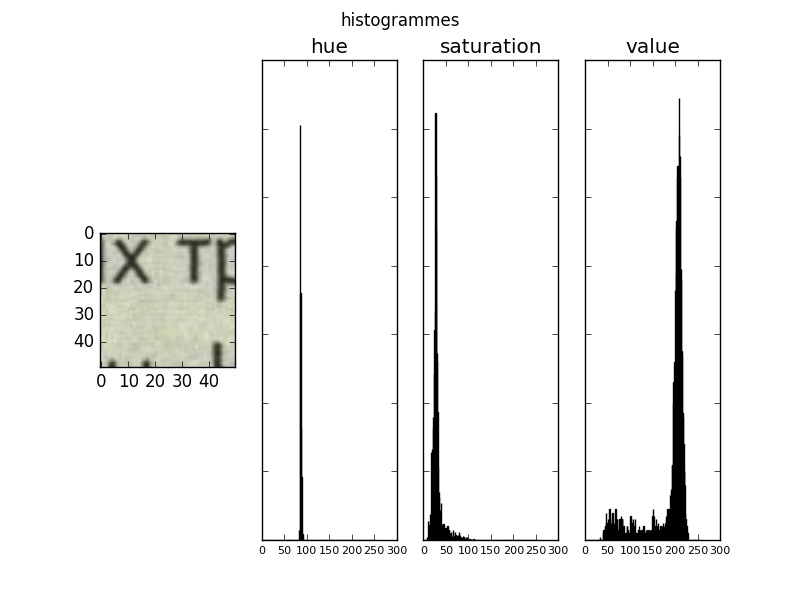
\includegraphics[scale=0.3]{images/histo_hsv_texte.jpg}
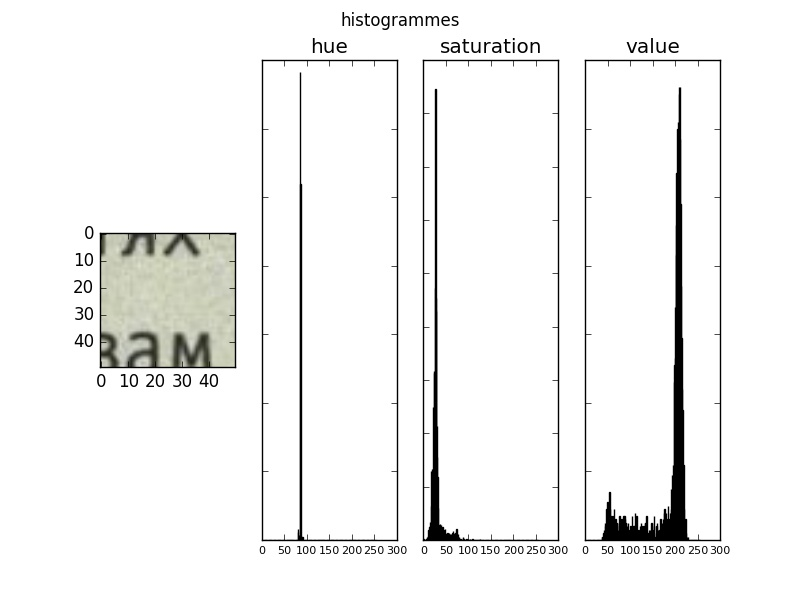
\includegraphics[scale=0.3]{images/histo_hsv_texte2.jpg}
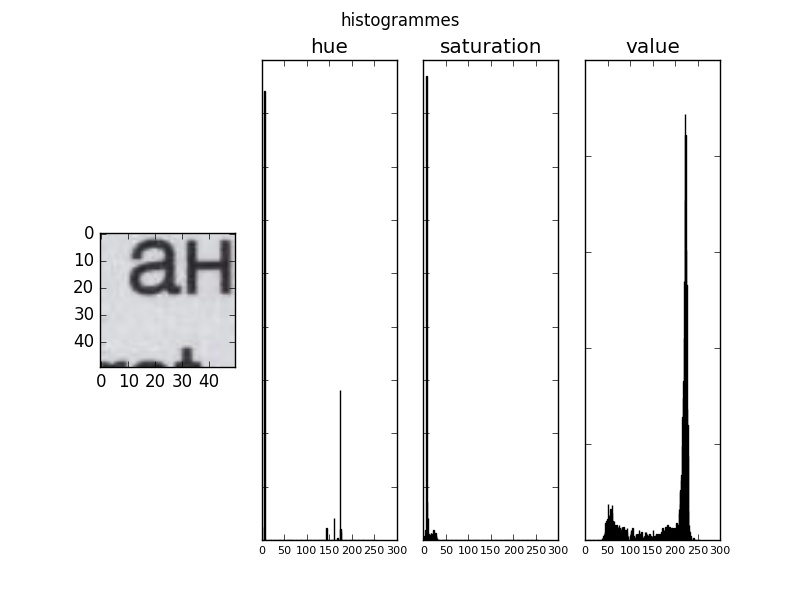
\includegraphics[scale=0.3]{images/histo_hsv_texte3.jpg}
\end{center}
\caption{histogrammes HSV pour trois patchs de texte}
\label{histo_hsv_texte}
\end{figure}


\chapter{Clustering}

A ce stade, nous avons des pixels qui ne sont pas du $fond$ et auxquels nous devons attribuer une classe parmi $texte$ et $illustration$.
Les features extraits au chapître précédents doivent donc être décomposer en deux sous groupes, à cet effet deux algorithmes sont utilisés :
\begin{description} % listes descriptives

\item[$KMeans$ :] cet algorithme permet de créer deux amas compactes par minimisation de l'énergie intra-cluster.
\item[$NMF$ (\begin{itshape}Non-Negative Matrix Factorization\end{itshape} :] cet algorithme permet de projeter les features des N pixels. Ces features de dimension P seront projetés sur un espace à 2 dimensions positives. On crééra ensuite
deux amas : un premier pour les points dont la première composante de projection est plus grande que la seconde, un second pour les autres.

\end{description}

A l'issue de cette étape de classification, nous avons donc deux amas de pixels. Nous définirons comme $texte$, l'amas de pixels dont la proportion de pixels blancs
est la plus grande. En effet, le texte possède plus de pixels blancs vu qu'il est très souvent écris sur fond blanc.\\
La figure \ref{resultat} montre l'application du $KMeans$ sur les descripteurs $HOG$+$HSV$ pour les pixels restants à déterminer.

\begin{figure}[H]
\begin{center}
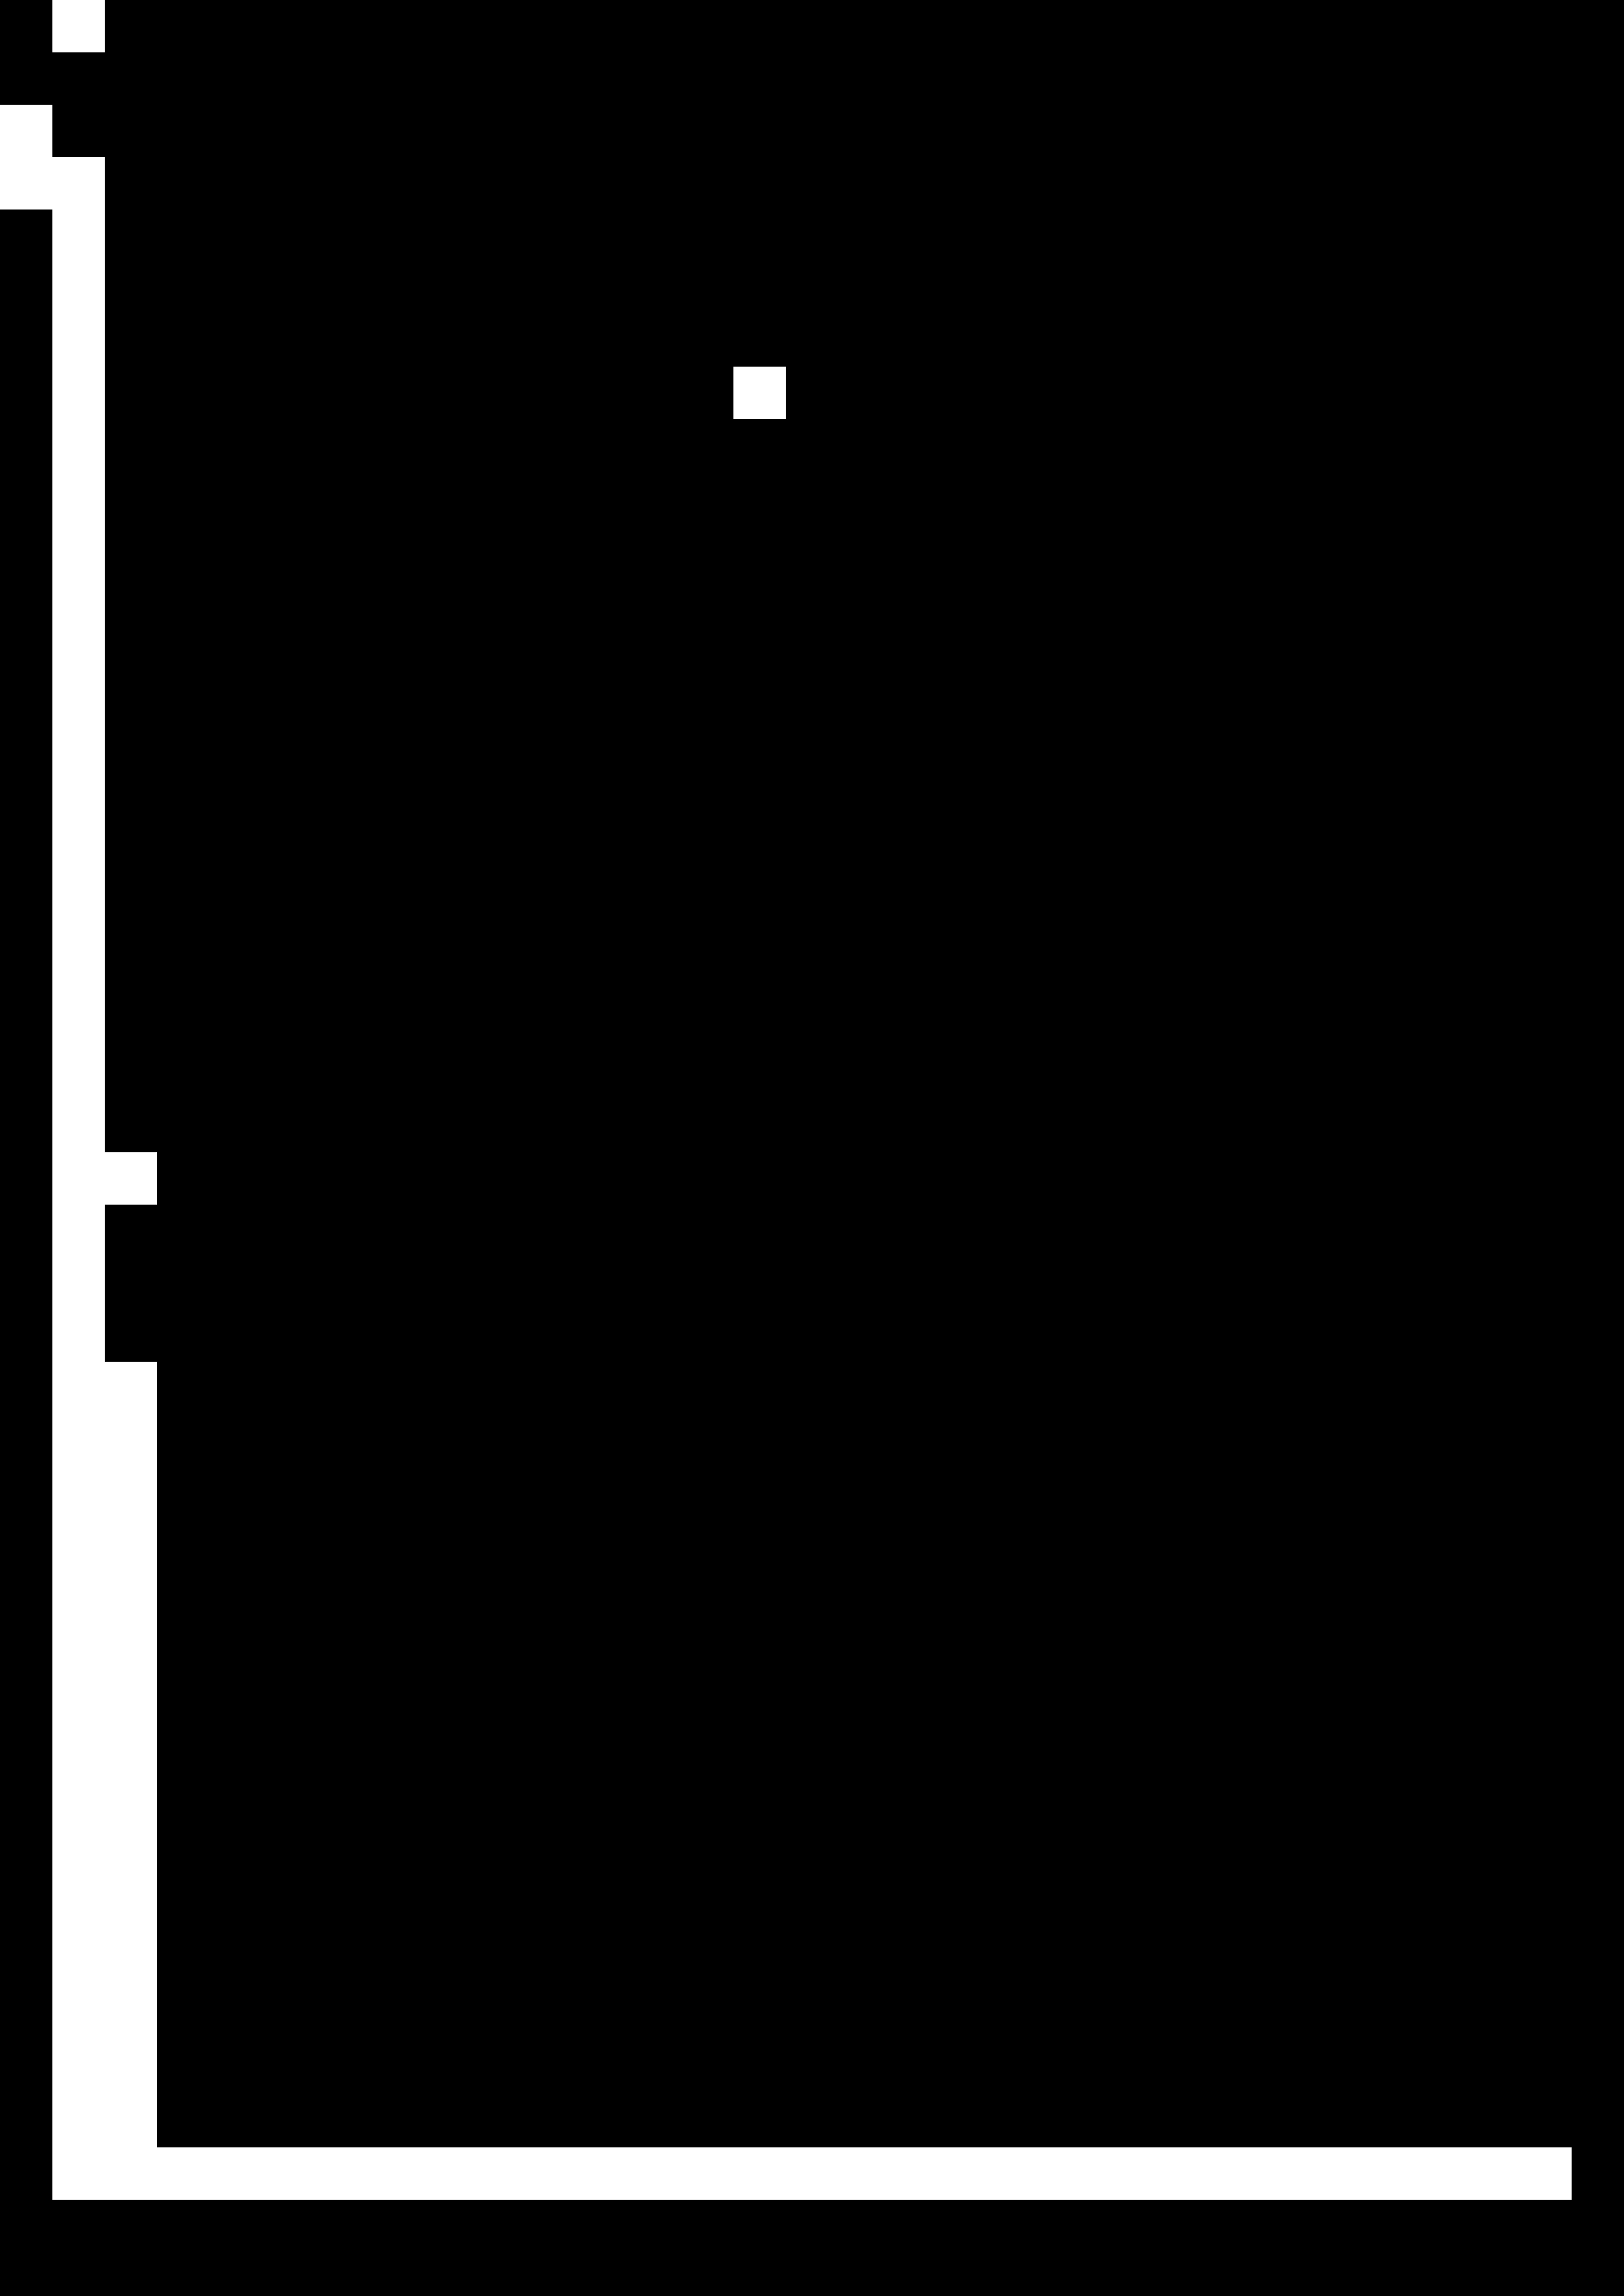
\includegraphics[scale=0.06]{images/1g_seuil.jpg}
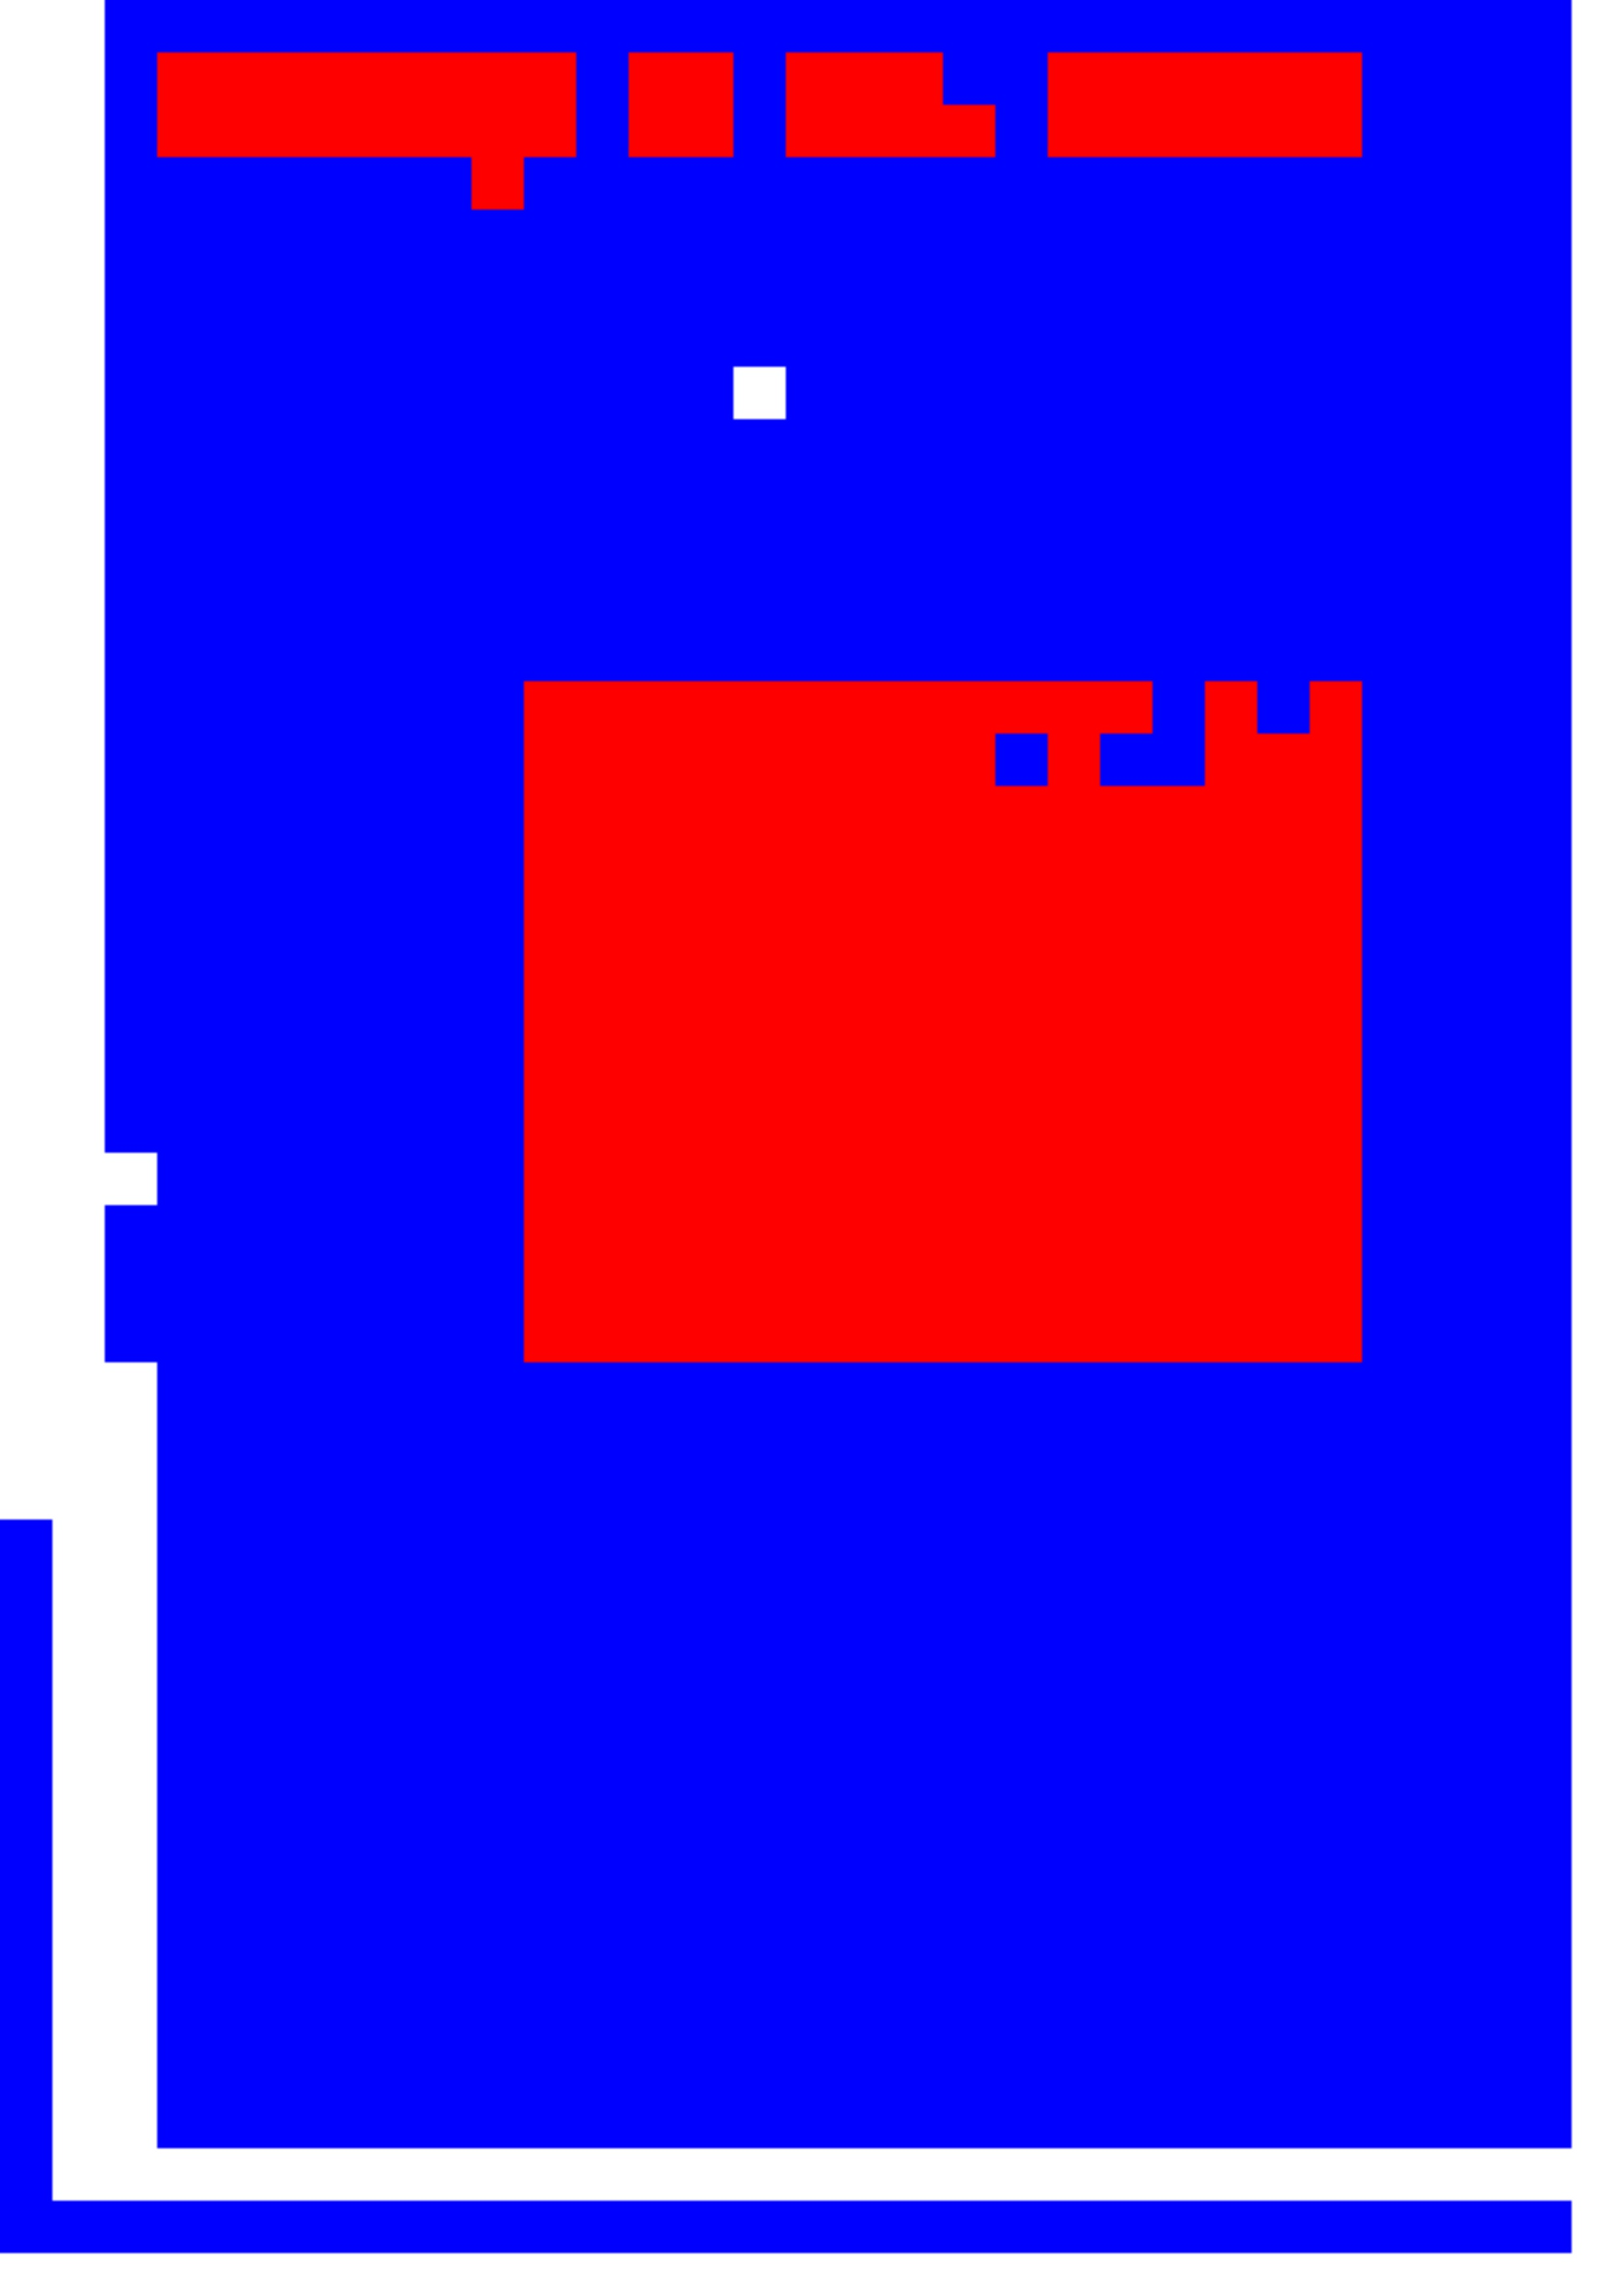
\includegraphics[scale=0.06]{images/1g_res_hog_hsv.jpg}
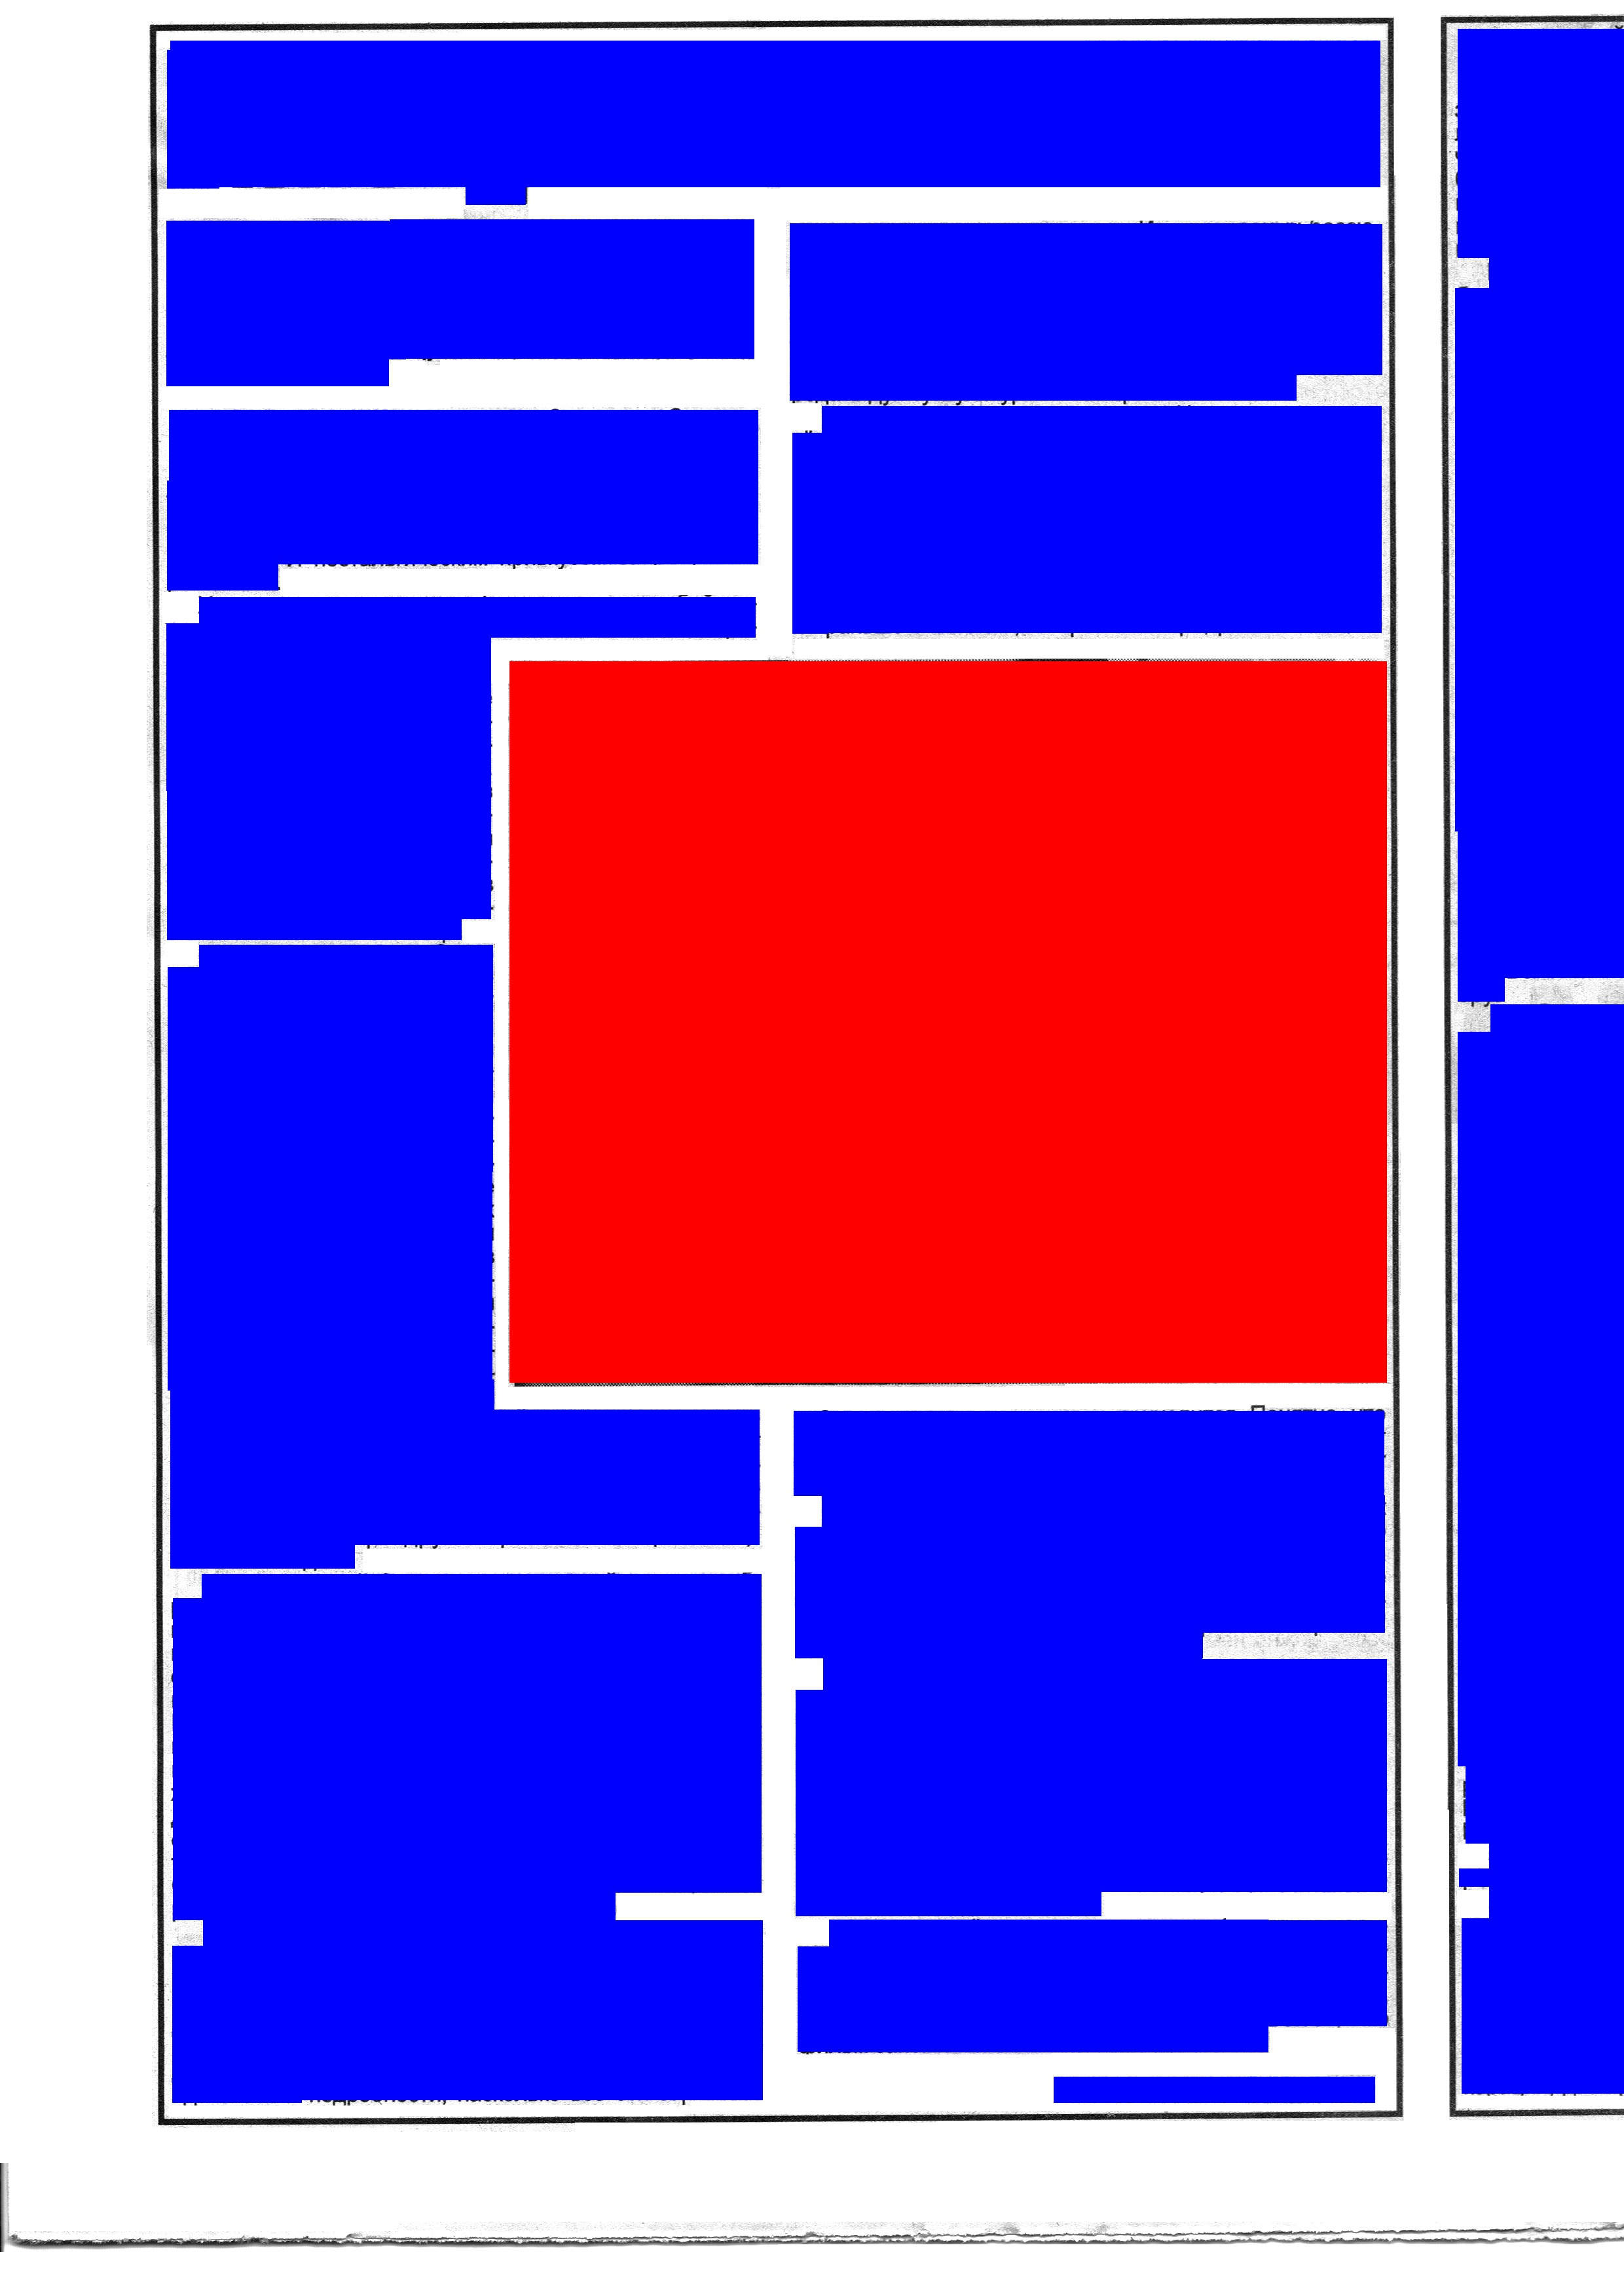
\includegraphics[scale=0.3]{images/1g_m.jpg}
\end{center}
\caption{attribution de la classe $illustration$ (rouge) ou $texte$ (bleu) par $KMeans$ sur les dscripteurs $HOG+HSV$ - en bas, la vérité terrain}
\label{resultat}
\end{figure}

\chapter{Précision/Rappel}

On applique le processus à toutes les images en procédant comme détaillé plus haut :

\begin{description}
 \item[-] Seuillage afin de déterminer les pixels de classe $fond$
 \item[-] Extraction de features des pixels restants (pour chaque pixel, concaténation du vecteur descripteurs HOG (ou Laplacien) et du vecteur descripteur HSV)
 \item[-] Clusterisation des features afin de déterminer la classe $illustration$ ou $texte$ des pixels restants
\end{description}

A des fins de mesures des performances, on utilise la vérité-terrain pour le calcul de précision/rappel pour chaque classe.\\
\ref{res_classe1},\ref{res_classe2} et \ref{res_classe3} récapitulent les precision/rappel obtenus respectivement pour les classes $fond$,$texte$ et $illustration$.
A noter que la classe fond est déterminé au début du processus par seuillage, et ne dépend donc pas des descripteurs et de la décomposition utilisé ensuite
pour déterminer le $texte$ et les $illustrations$
\begin{table}
\begin{center}
%\begin{tabular}{|p{5cm}|p{2cm}|p{2cm}|p{2cm}|p{2cm}|}
\begin{tabular}{|c|c|}
\hline
\begin{bf}precision\end{bf} & \begin{bf}recall\end{bf}\\
\hline
0.55 & 0.90\\
\hline
\end{tabular}
\end{center}
\caption{precision/rappel pour la classe $fond$}
\label{res_classe1}
\end{table}

\begin{table}
\begin{center}
%\begin{tabular}{|p{5cm}|p{2cm}|p{2cm}|p{2cm}|p{2cm}|}
\begin{tabular}{|c|c|c|c|c|}
\hline
\multirow{\begin{bf}Descripteurs\end{bf}} & \multicolumn{2}{c|}{\begin{bf}KMeans\end{bf}} & \multicolumn{2}{c|}{\begin{bf}NMF\end{bf}}\\
\cline{2-5} & \begin{bf}precision\end{bf} & \begin{bf}recall\end{bf} & \begin{bf}precision\end{bf} & \begin{bf}recall\end{bf}\\
\hline
$Laplacien+HSV$ & 0.63 & 0.55 & 0.38 & 0.40\\
\hline
$HOG+HSV$ &  0.64 & 0.61 & 0.39 & 0.47\\
\hline
\end{tabular}
\end{center}
\caption{precision/rappel pour la classe $illustration$}
\label{res_classe2}
\end{table}

\begin{table}
\begin{center}
%\begin{tabular}{|p{5cm}|p{2cm}|p{2cm}|p{2cm}|p{2cm}|}
\begin{tabular}{|c|c|c|c|c|}
\hline
\multirow{\begin{bf}Descripteurs\end{bf}} & \multicolumn{2}{c|}{\begin{bf}KMeans\end{bf}} & \multicolumn{2}{c|}{\begin{bf}NMF\end{bf}}\\
\cline{2-5} & \begin{bf}precision\end{bf} & \begin{bf}recall\end{bf} & \begin{bf}precision\end{bf} & \begin{bf}recall\end{bf}\\
\hline
$Laplacien+HSV$ & 0.83 & 0.65 & 0.53 & 0.58\\
\hline
$HOG+HSV$ & 0.87 & 0.66 & 0.75 & 0.62\\
\hline
\end{tabular}
\end{center}
\caption{precision/rappel pour la classe $texte$}
\label{res_classe3}
\end{table}

\clearpage

On observe les meilleurs résultats pour un partitionnement $KMeans$ du descripteur $HOG+HSV$. Ainsi, la precision moyenne (toute image et toute classe confondue) est de 
\begin{bf}0.68\end{bf} et le rappel moyen de \begin{bf}0.72\end{bf}.\\
La figure \ref{meilleur_precision} présente l'image donnant la meilleure précision (\begin{bf}0.853\end{bf}).\\
La figure \ref{meilleur_rappel} présente l'image donnant le meilleur rappel (\begin{bf}0.902\end{bf}).\\

\begin{figure}[H]
\begin{center}
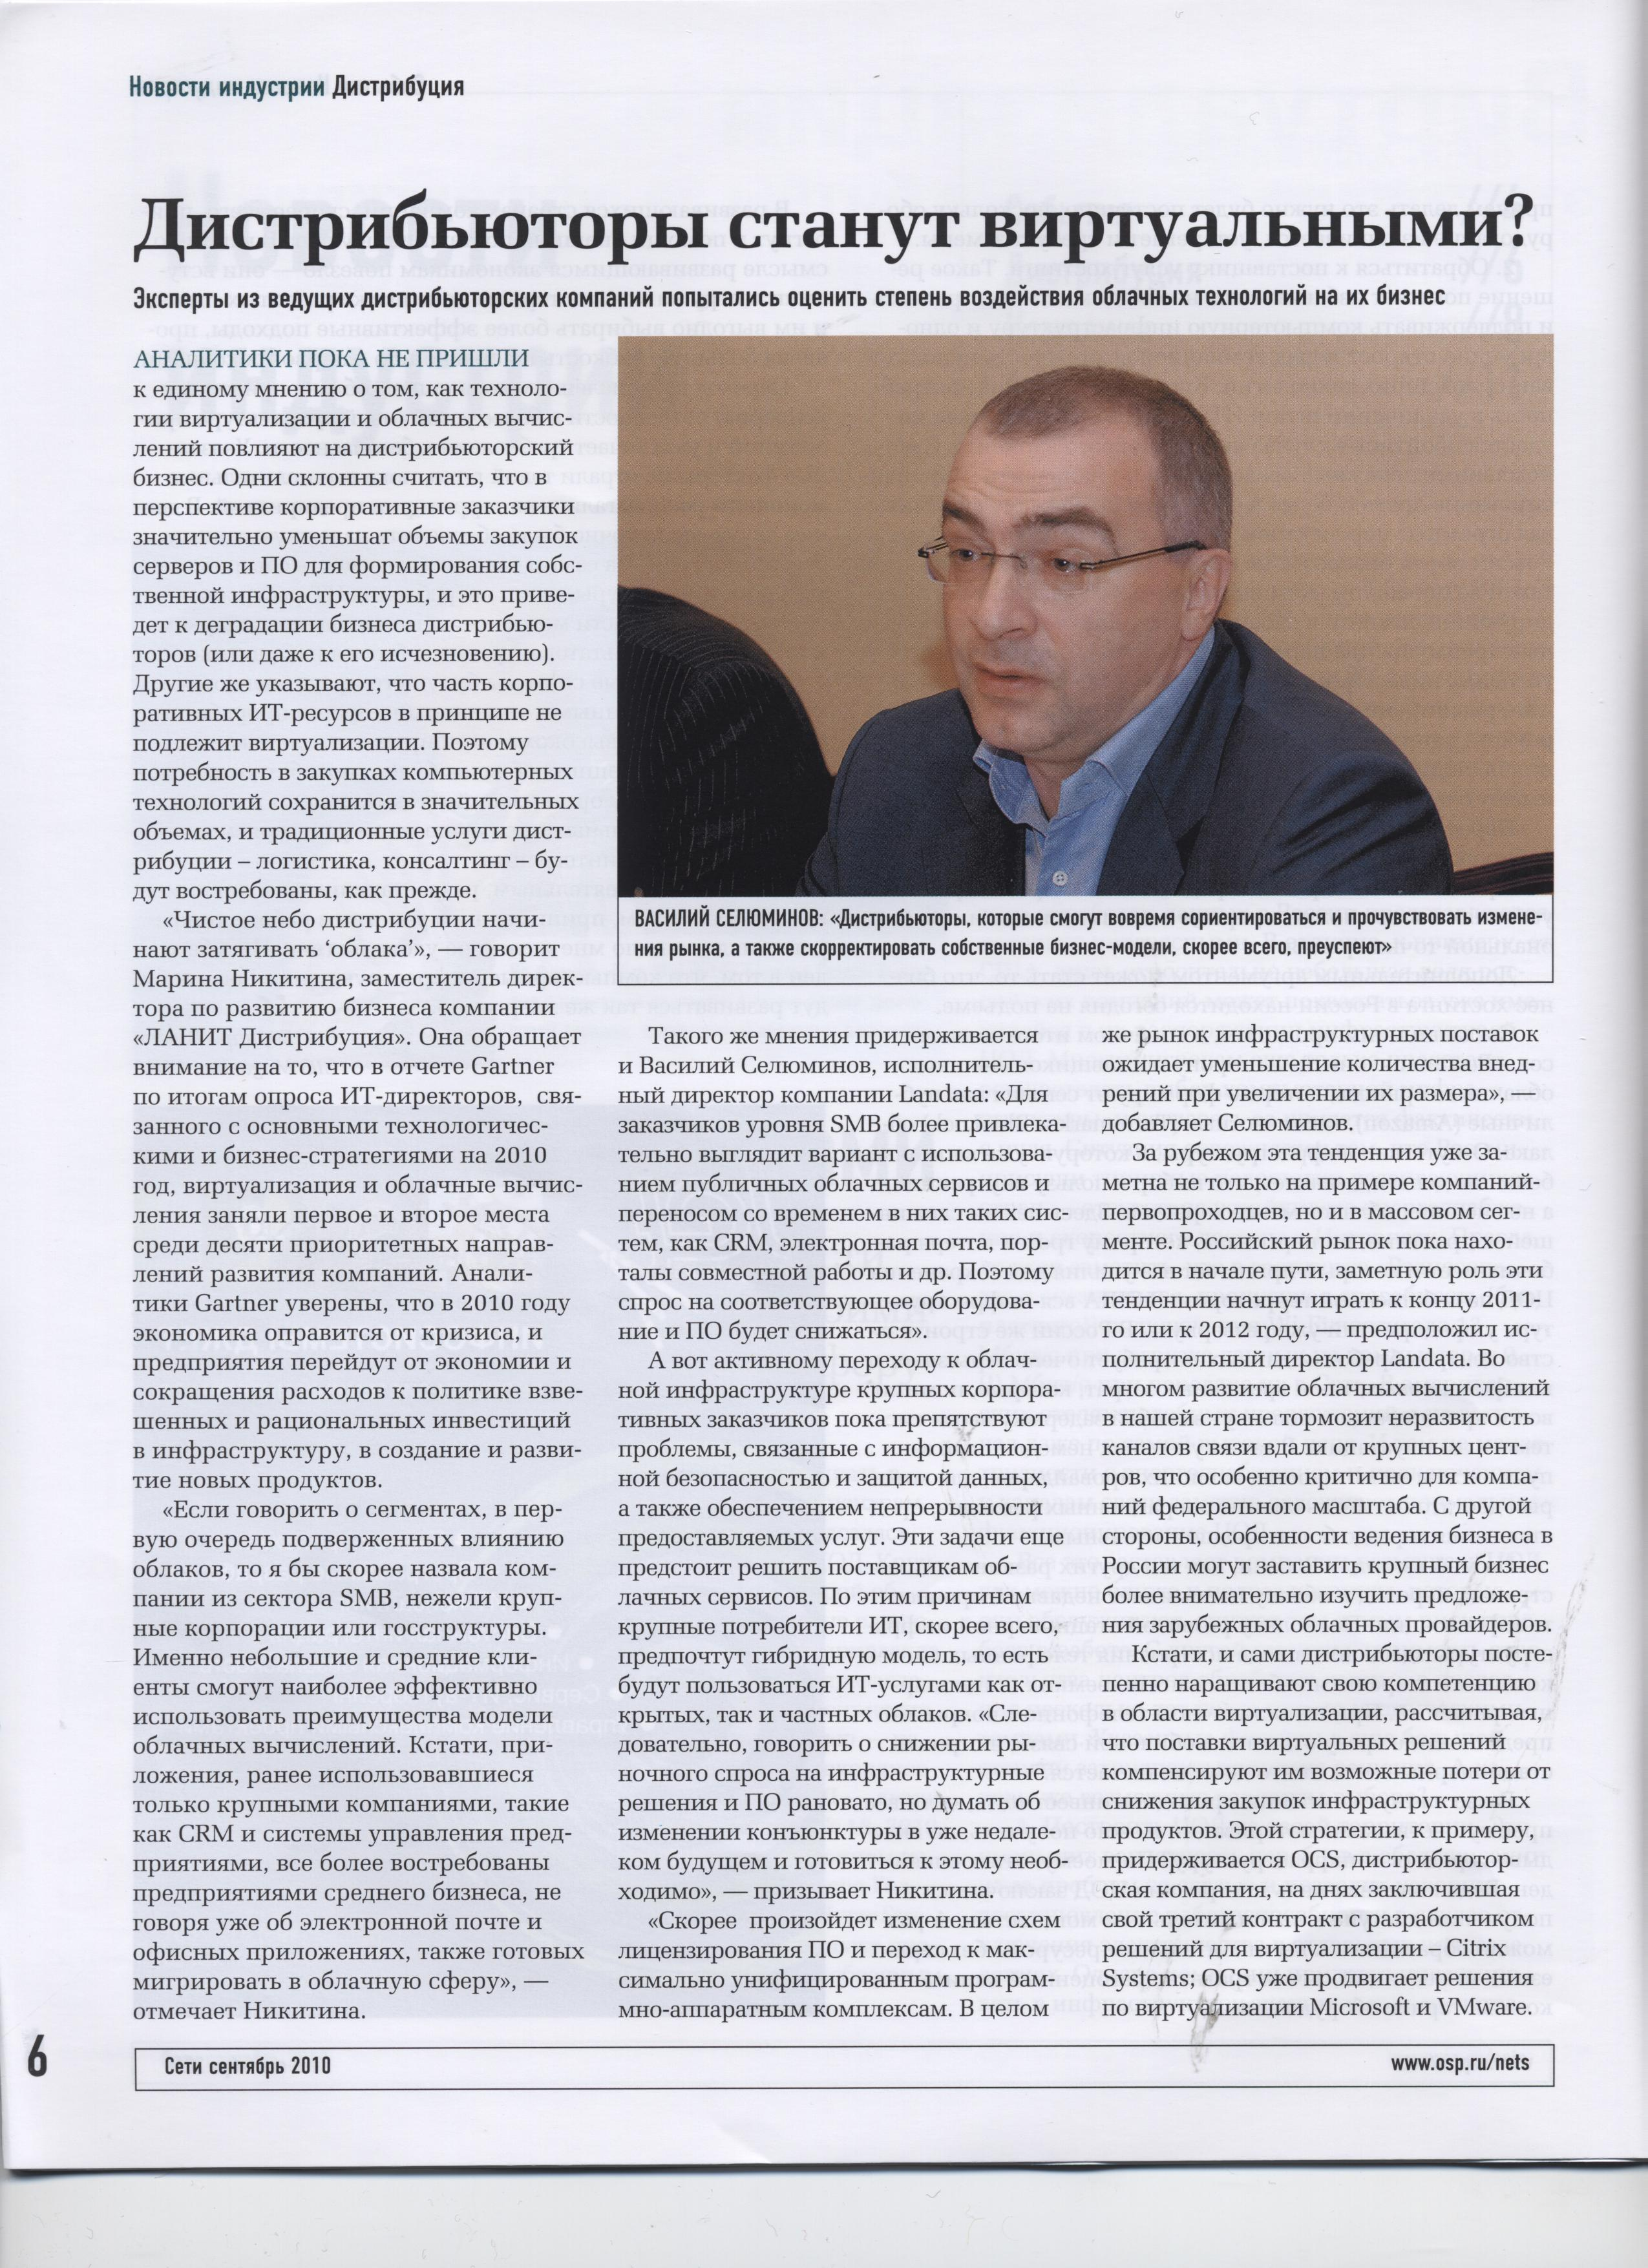
\includegraphics[scale=0.25]{images/20.jpg}
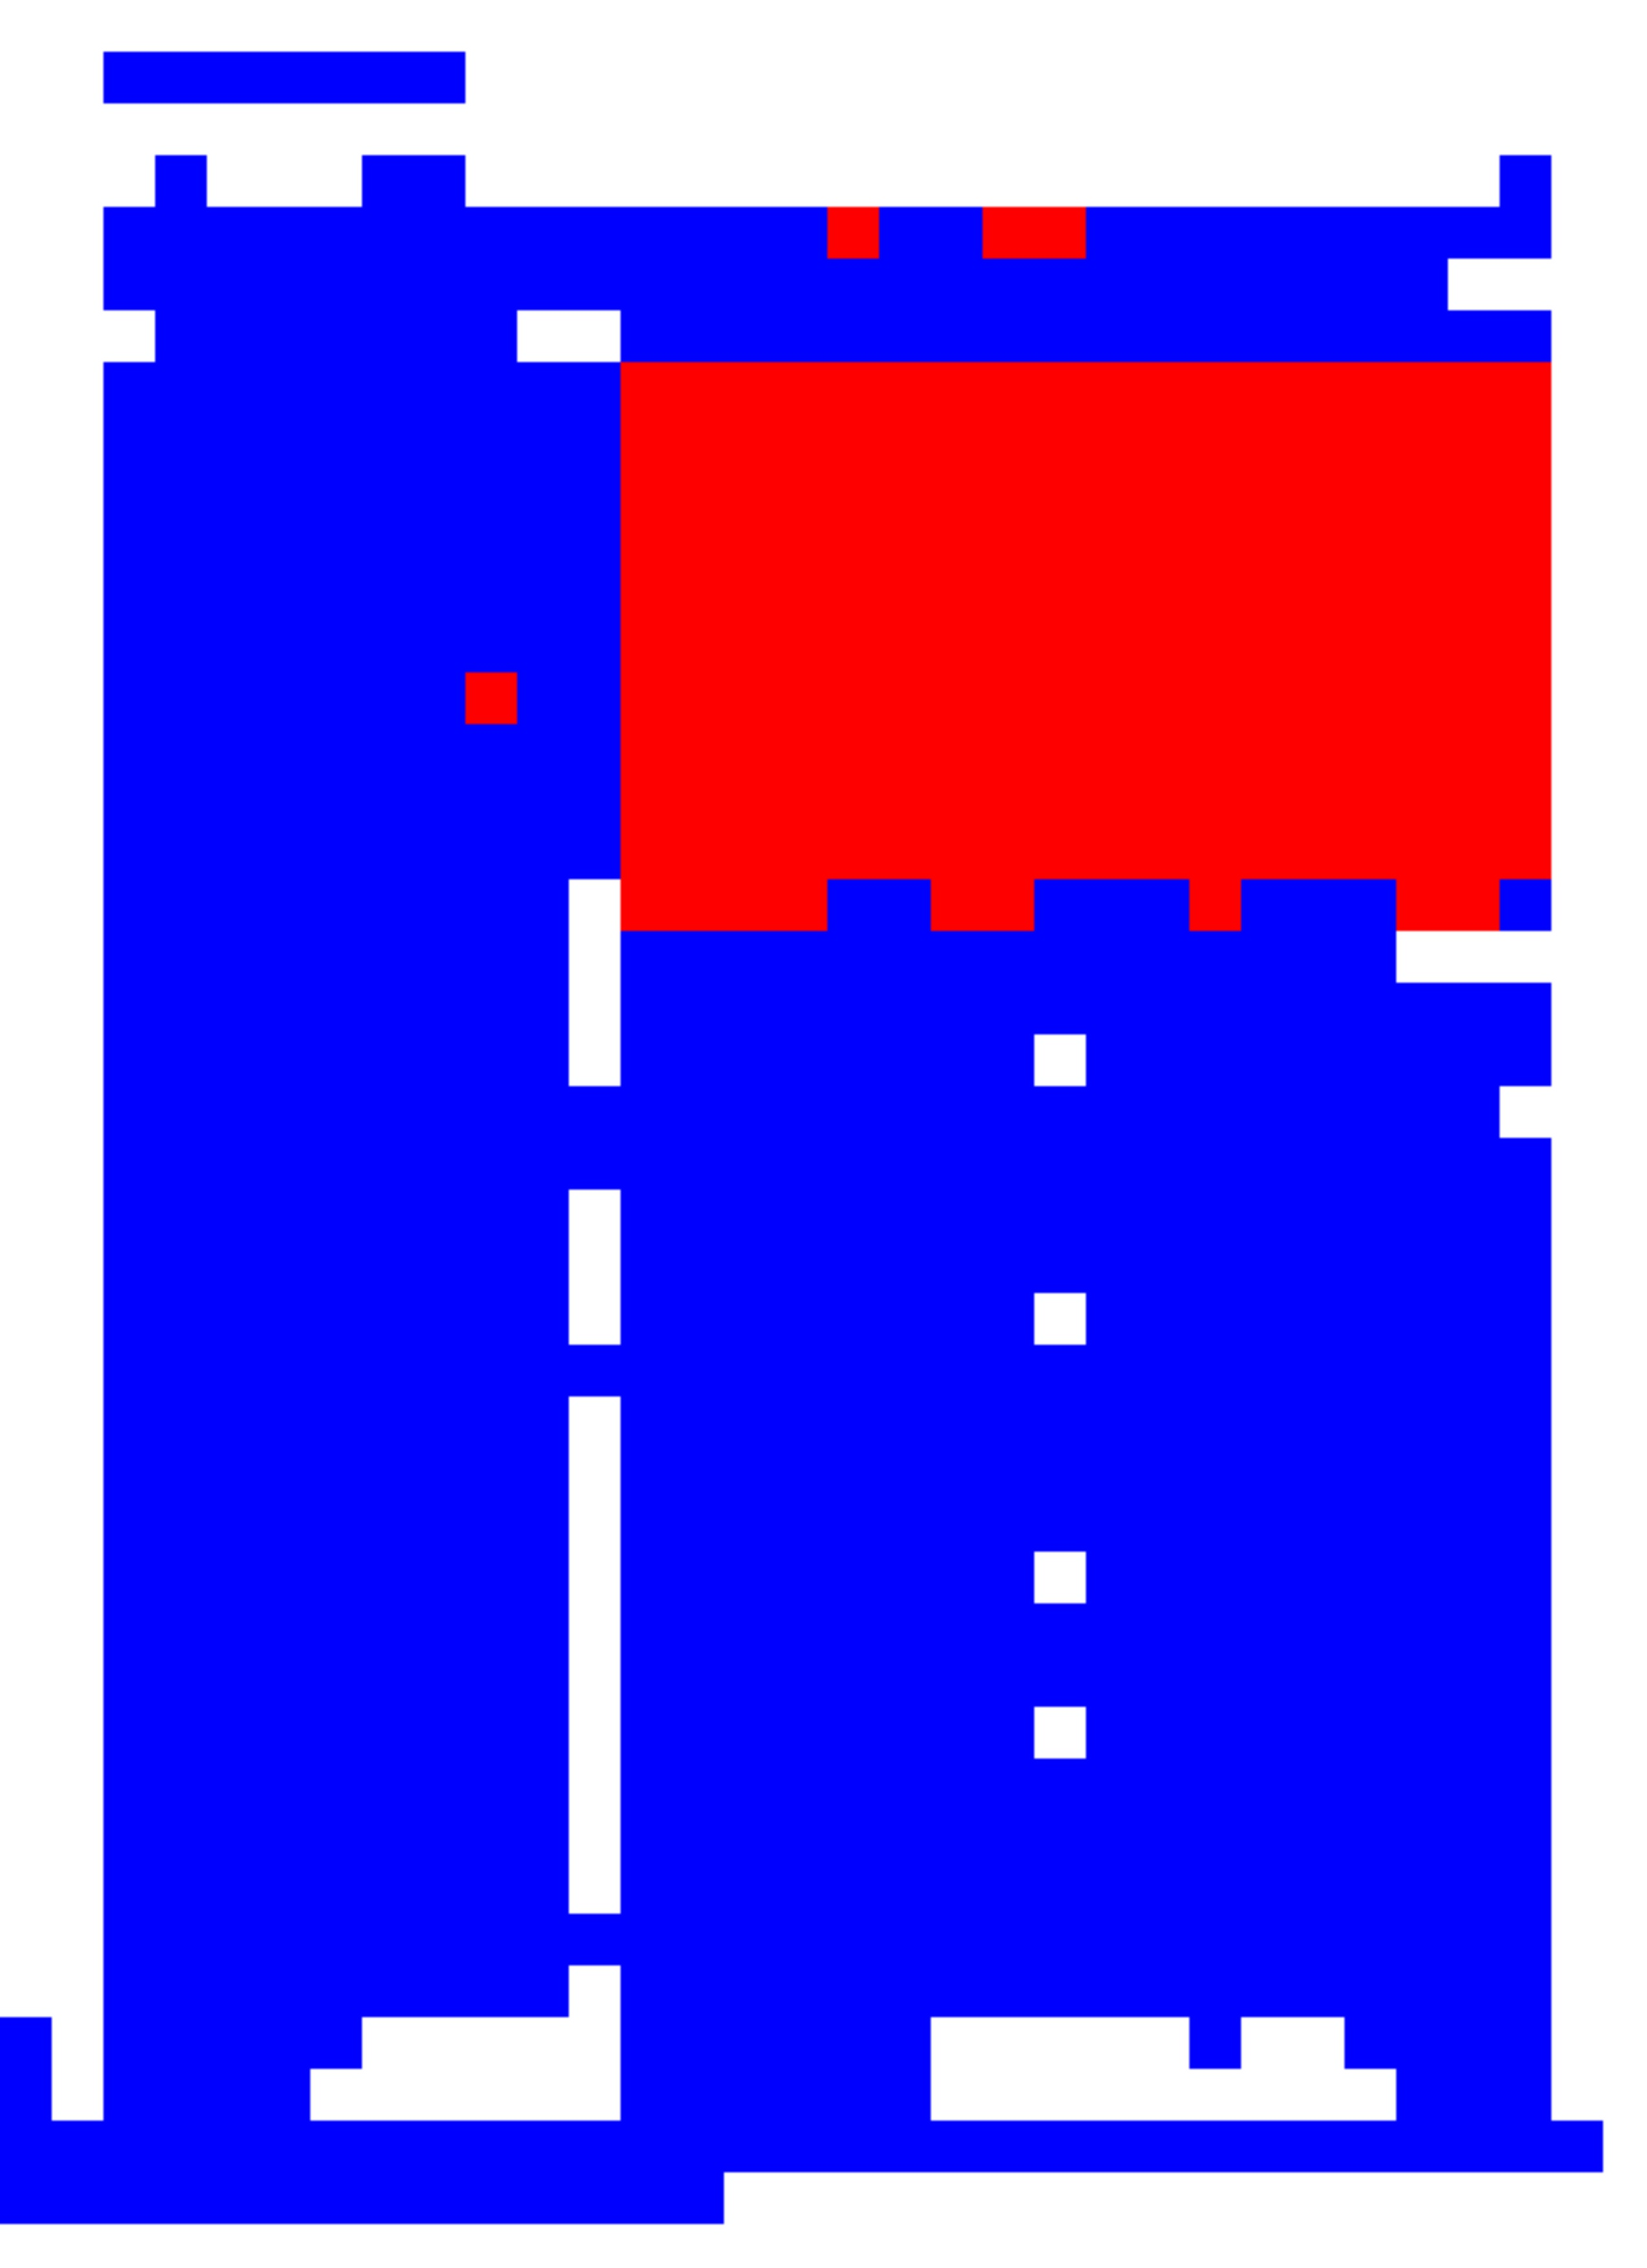
\includegraphics[scale=0.06]{images/20_res_hog_hsv_kmeans.jpg}
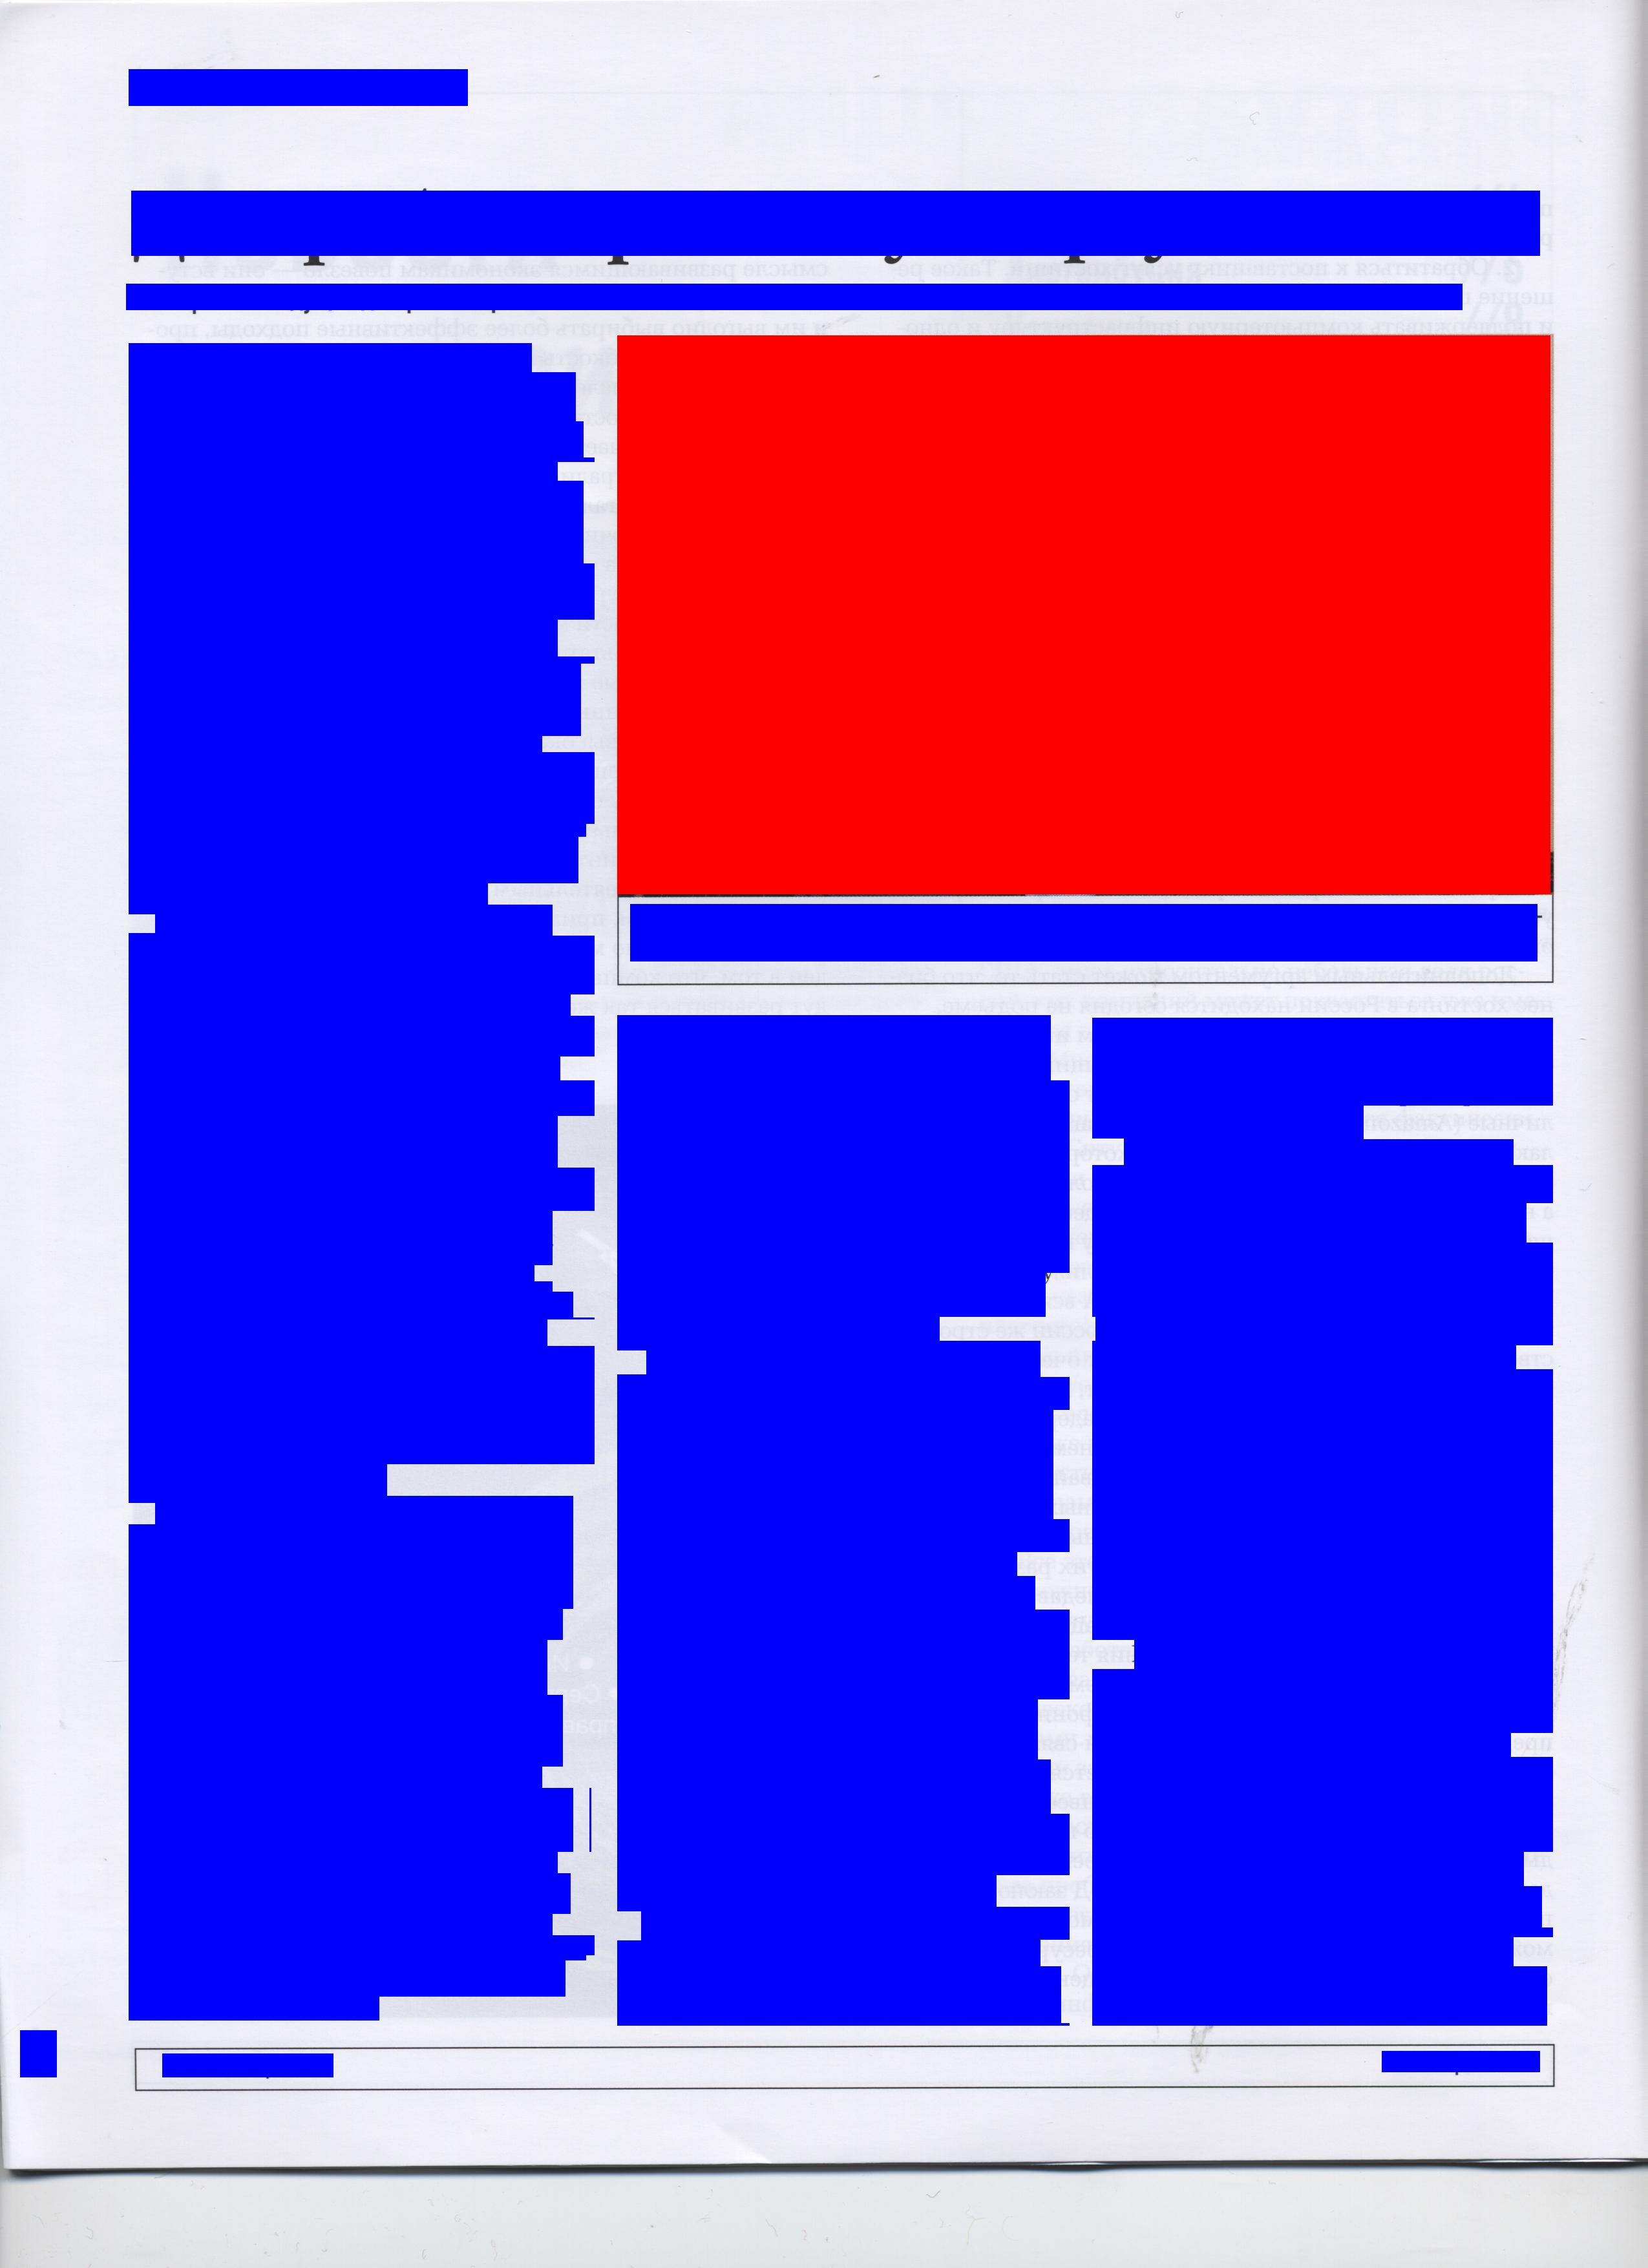
\includegraphics[scale=0.25]{images/20_m.jpg}
\end{center}
\caption{image donnant la précision moyenne maximale - en bas sa vérité-terrain}
\label{meilleur_precision}
\end{figure}

\begin{figure}[H]
\begin{center}
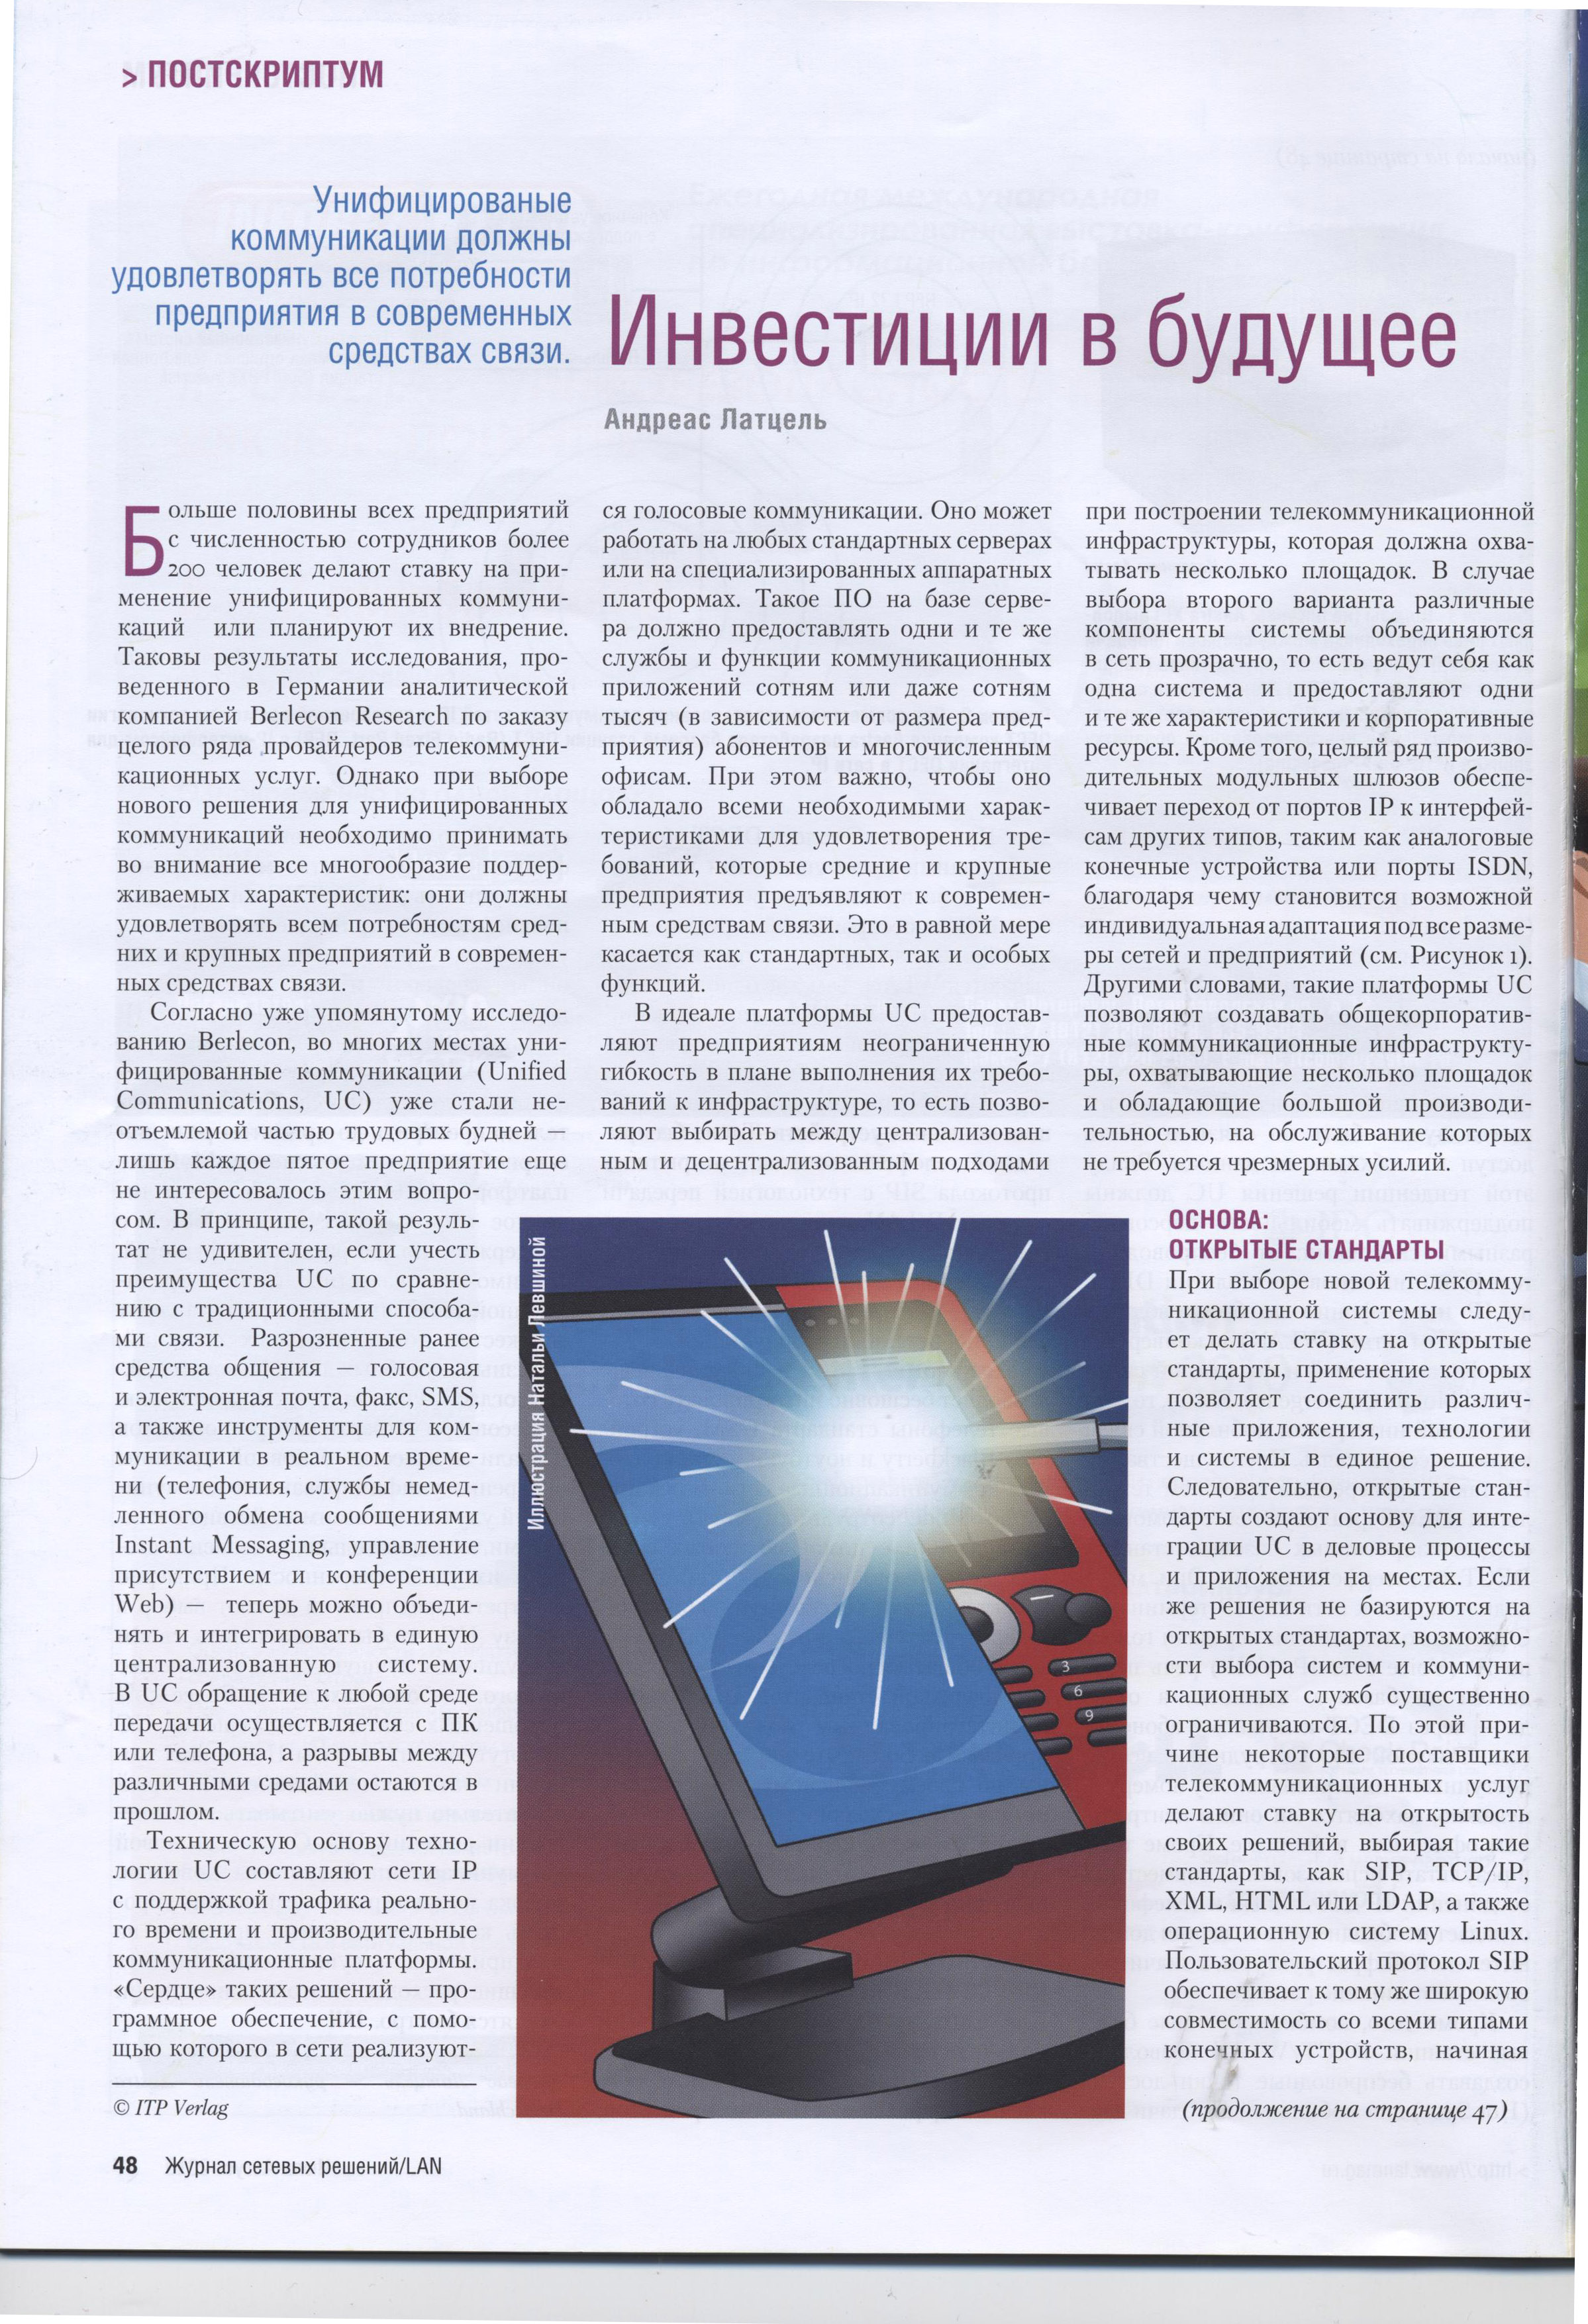
\includegraphics[scale=0.25]{images/50.jpg}
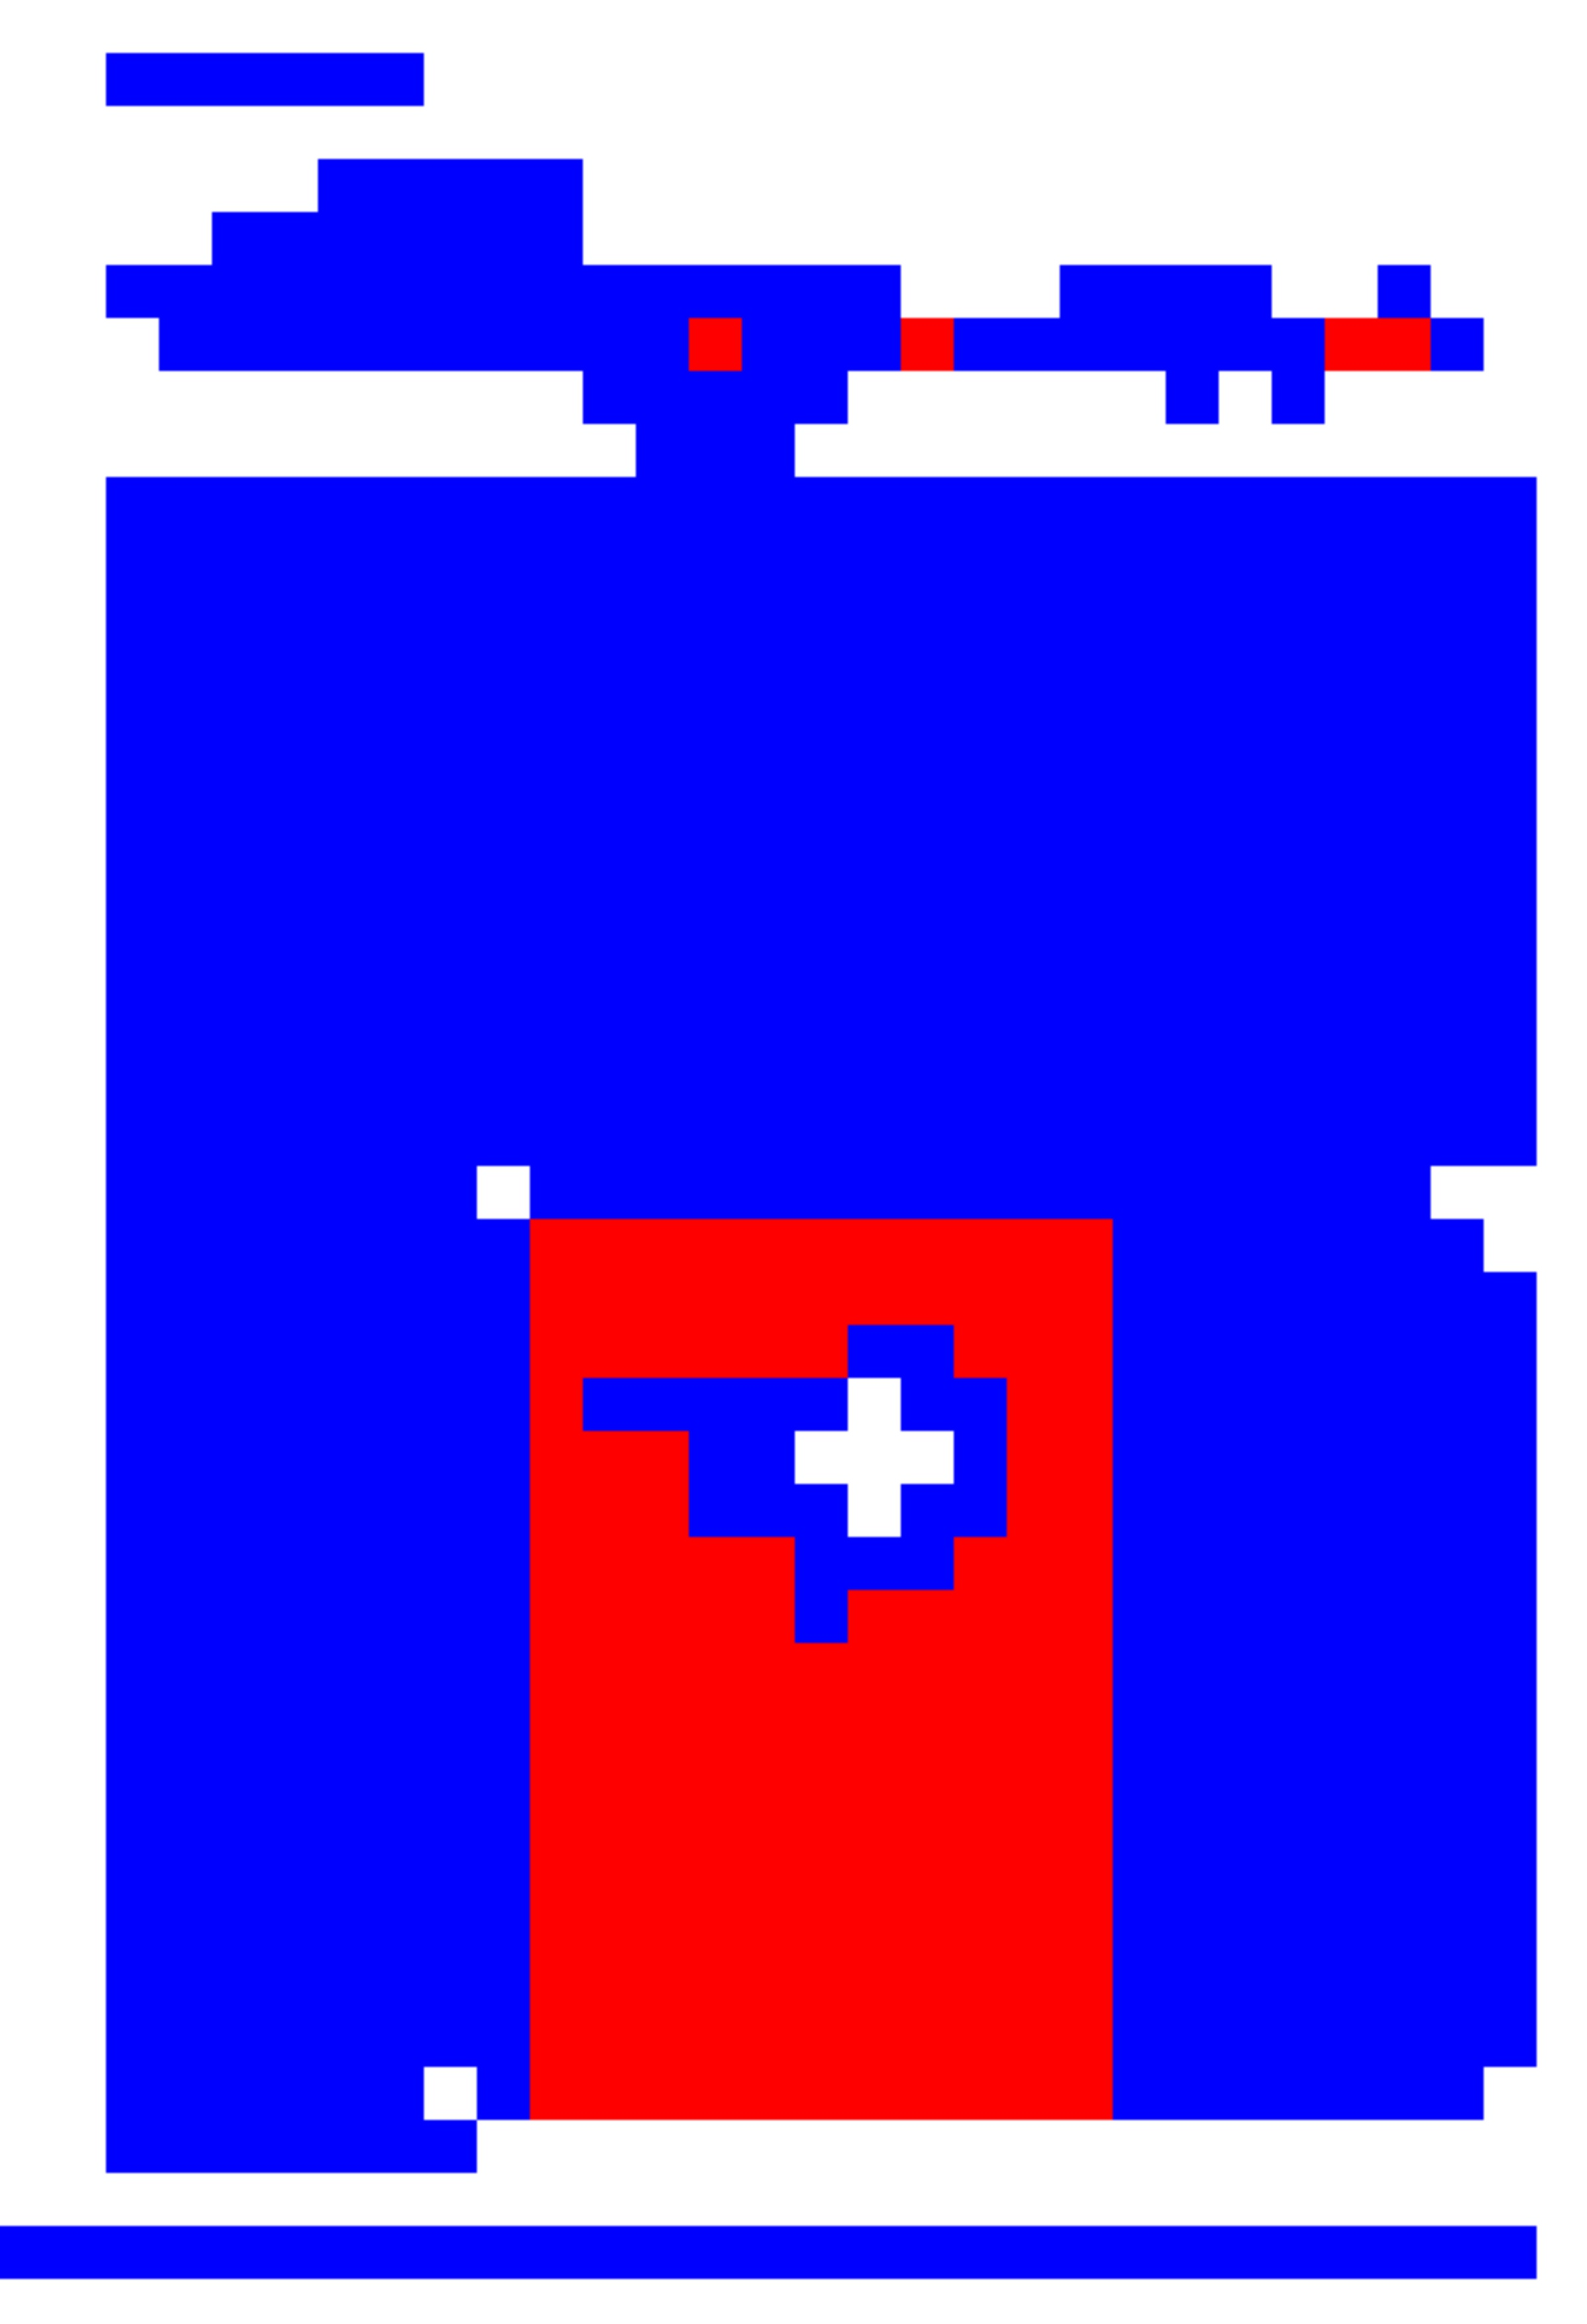
\includegraphics[scale=0.06]{images/50_res_hog_hsv_kmeans.jpg}
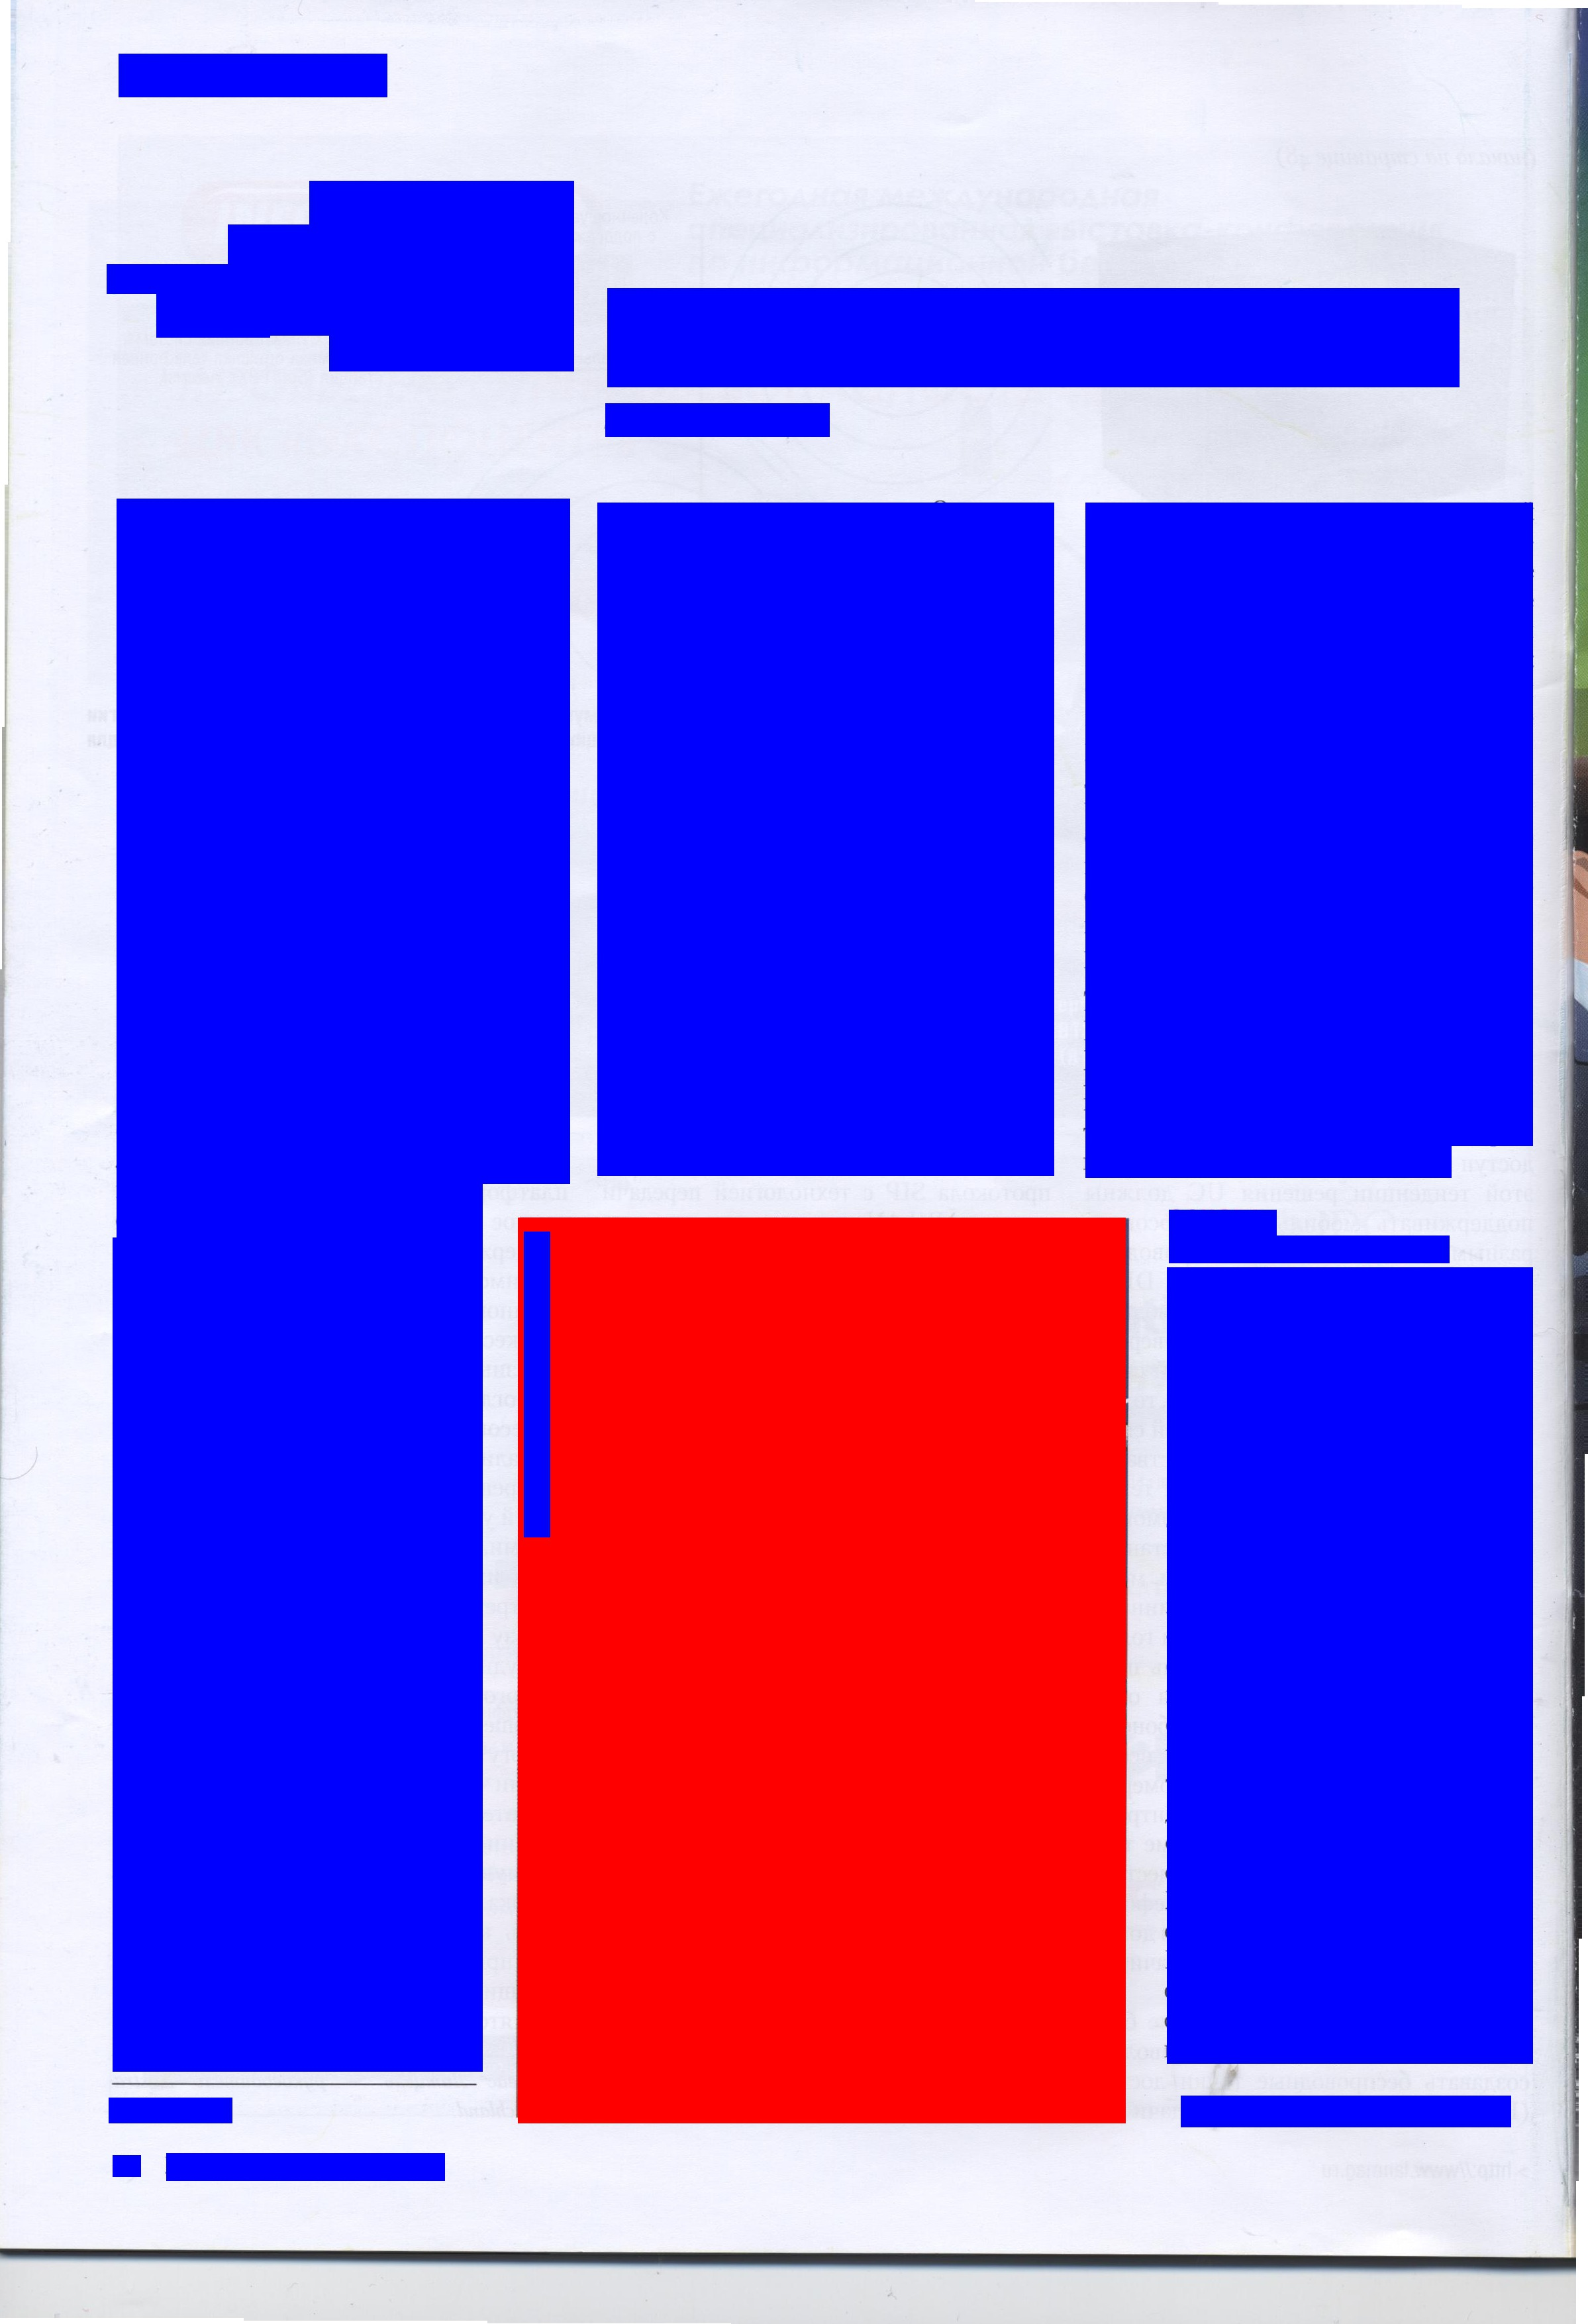
\includegraphics[scale=0.25]{images/50_m.jpg}
\end{center}
\caption{image donnant le rappel moyen maximal - en bas sa vérité-terrain}
\label{meilleur_rappel}
\end{figure}

\clearpage

\chapter{Test}

Nous avons cherché à verifier la généralité de notre méthode, en la testant sur des articles de revue numérisés provenant d'alphabets
différents.\\
Nous avons récupéré trois scans d'images prises totalement au hasard sur le net, en arabe, en hébreux et en japonais, les résultats
respectifs sont illustrés dans les figures \ref{test1} \ref{test2} \ref{test3}:\\ 

\begin{figure}[H]
\begin{center}
\includegraphics[scale=0.05]{../test/arabic.png}
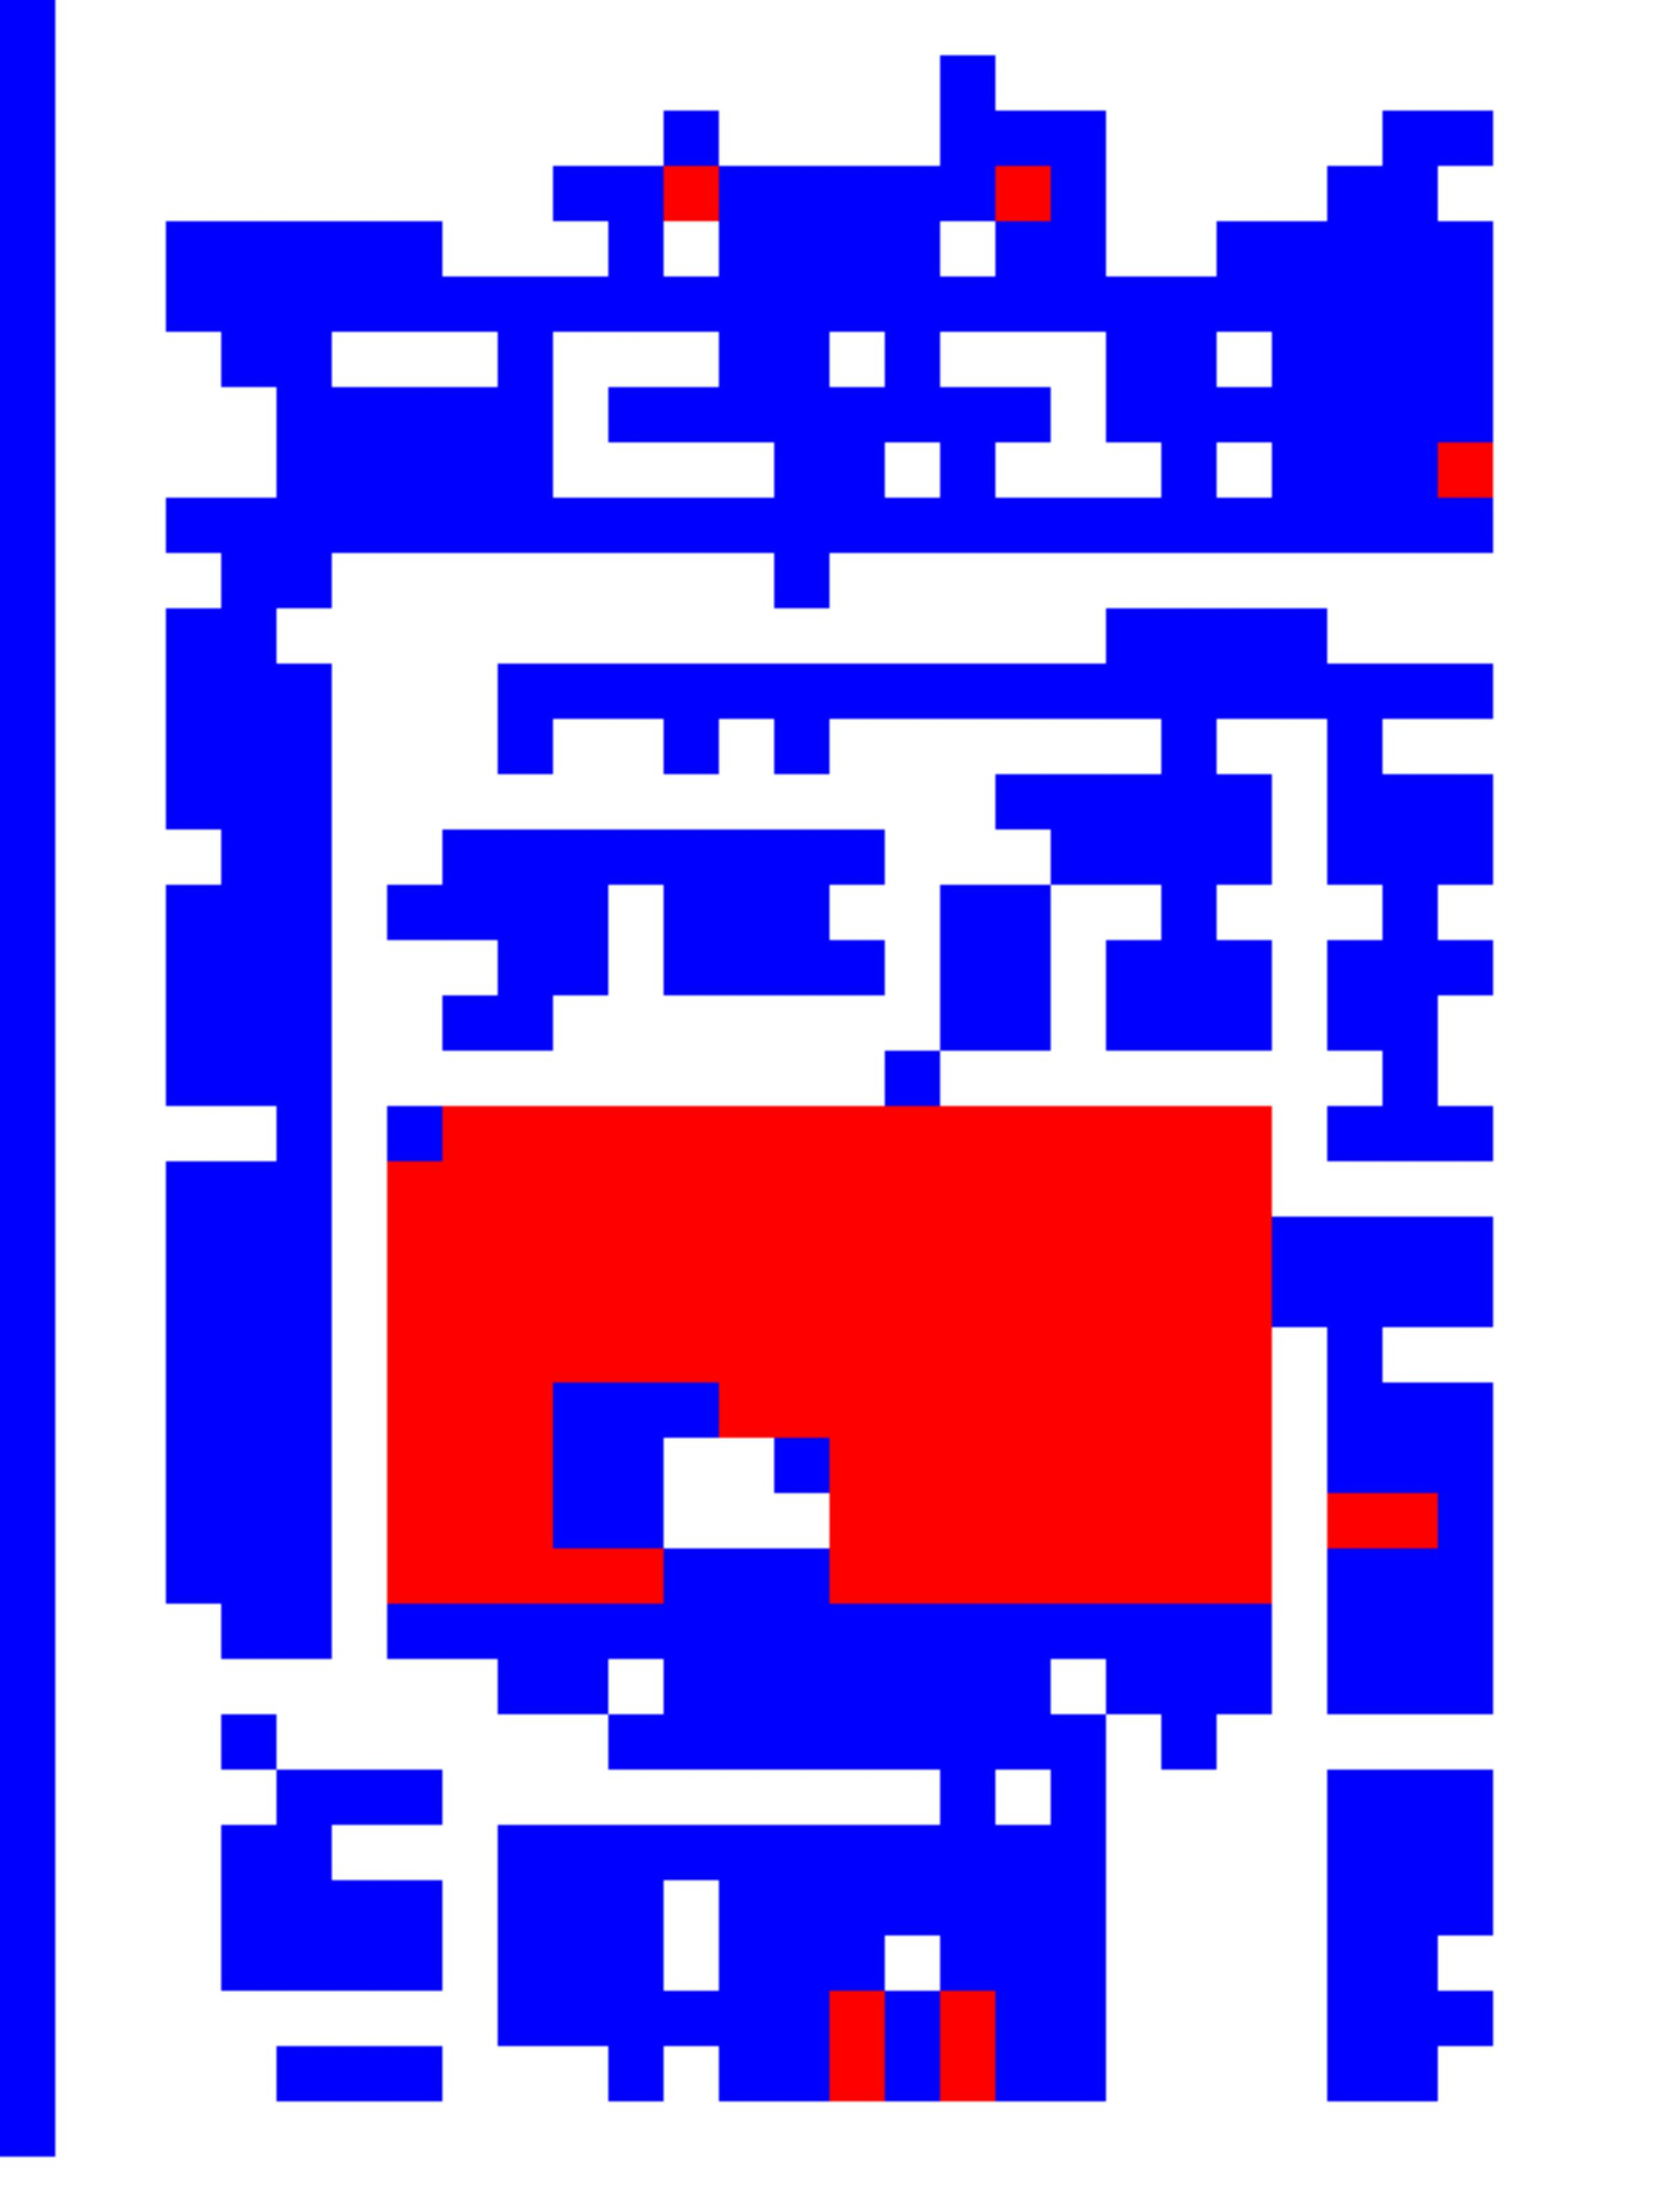
\includegraphics[scale=0.05]{../test/arabic_res_hog_hsv_kmeans.jpg}
\end{center}
\caption{test de la méthode sur l'image arabic.png}
\label{test1}
\end{figure}

\begin{figure}[H]
\begin{center}
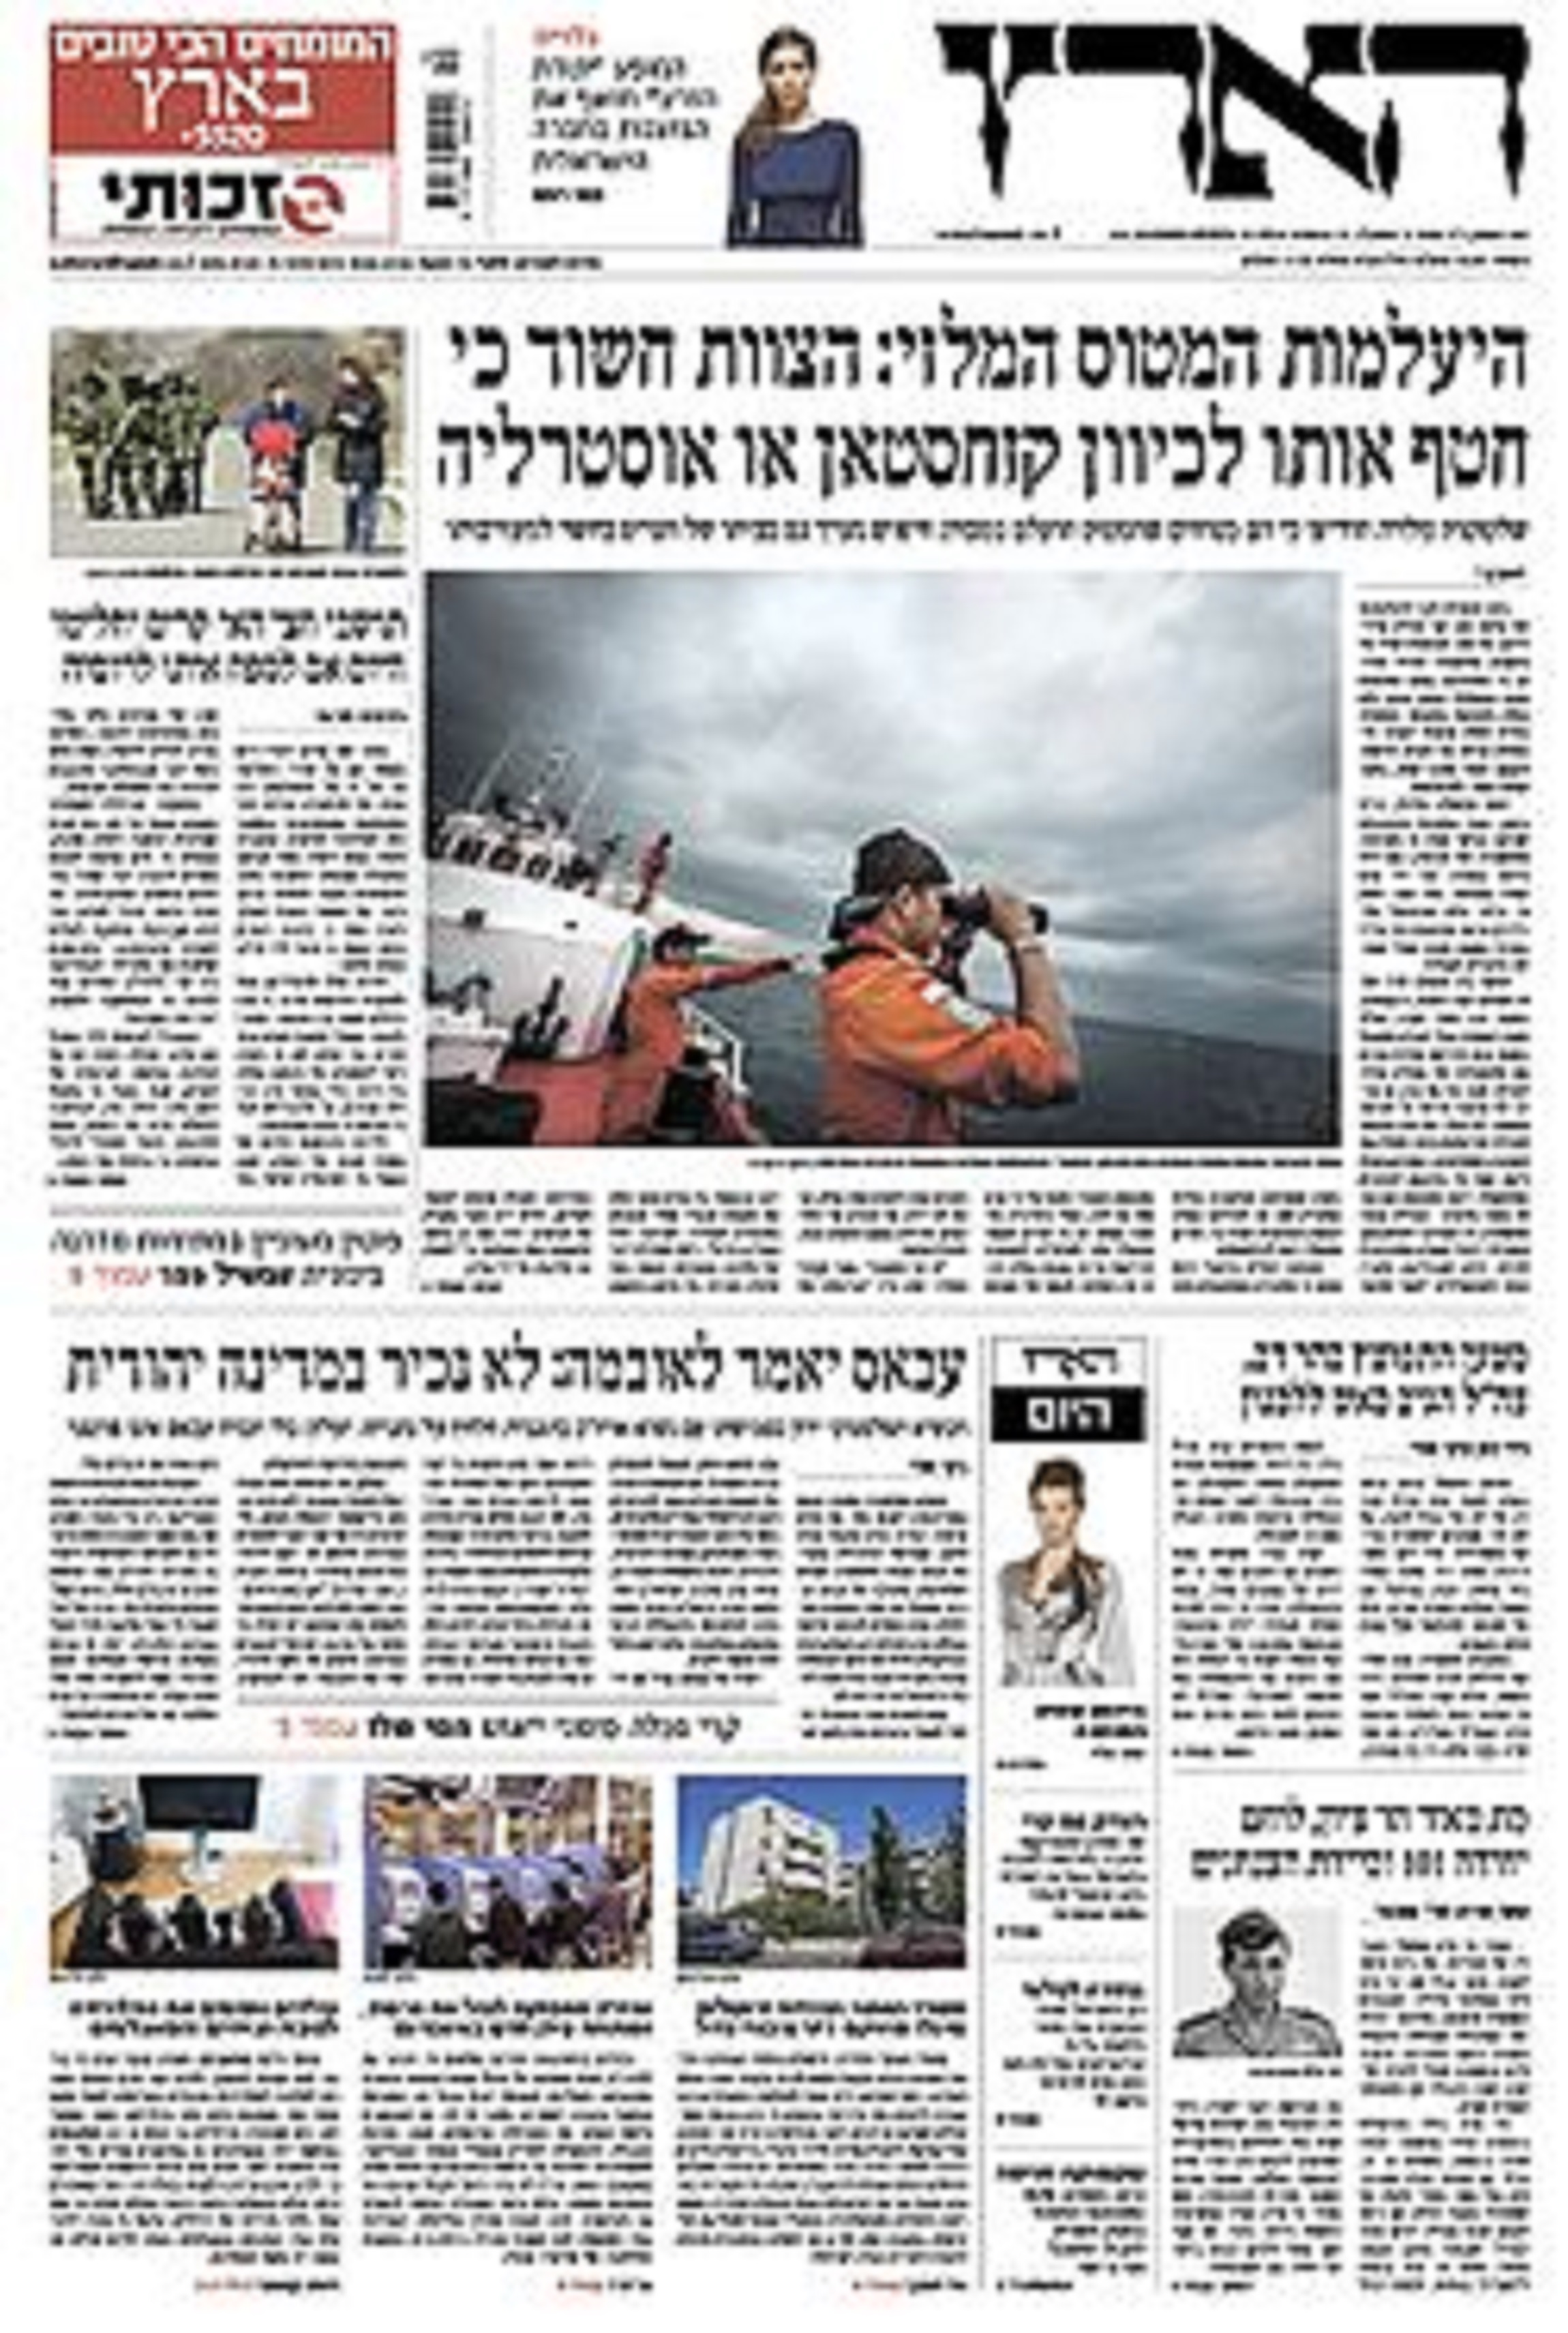
\includegraphics[scale=0.05]{../test/hebraic.jpg}
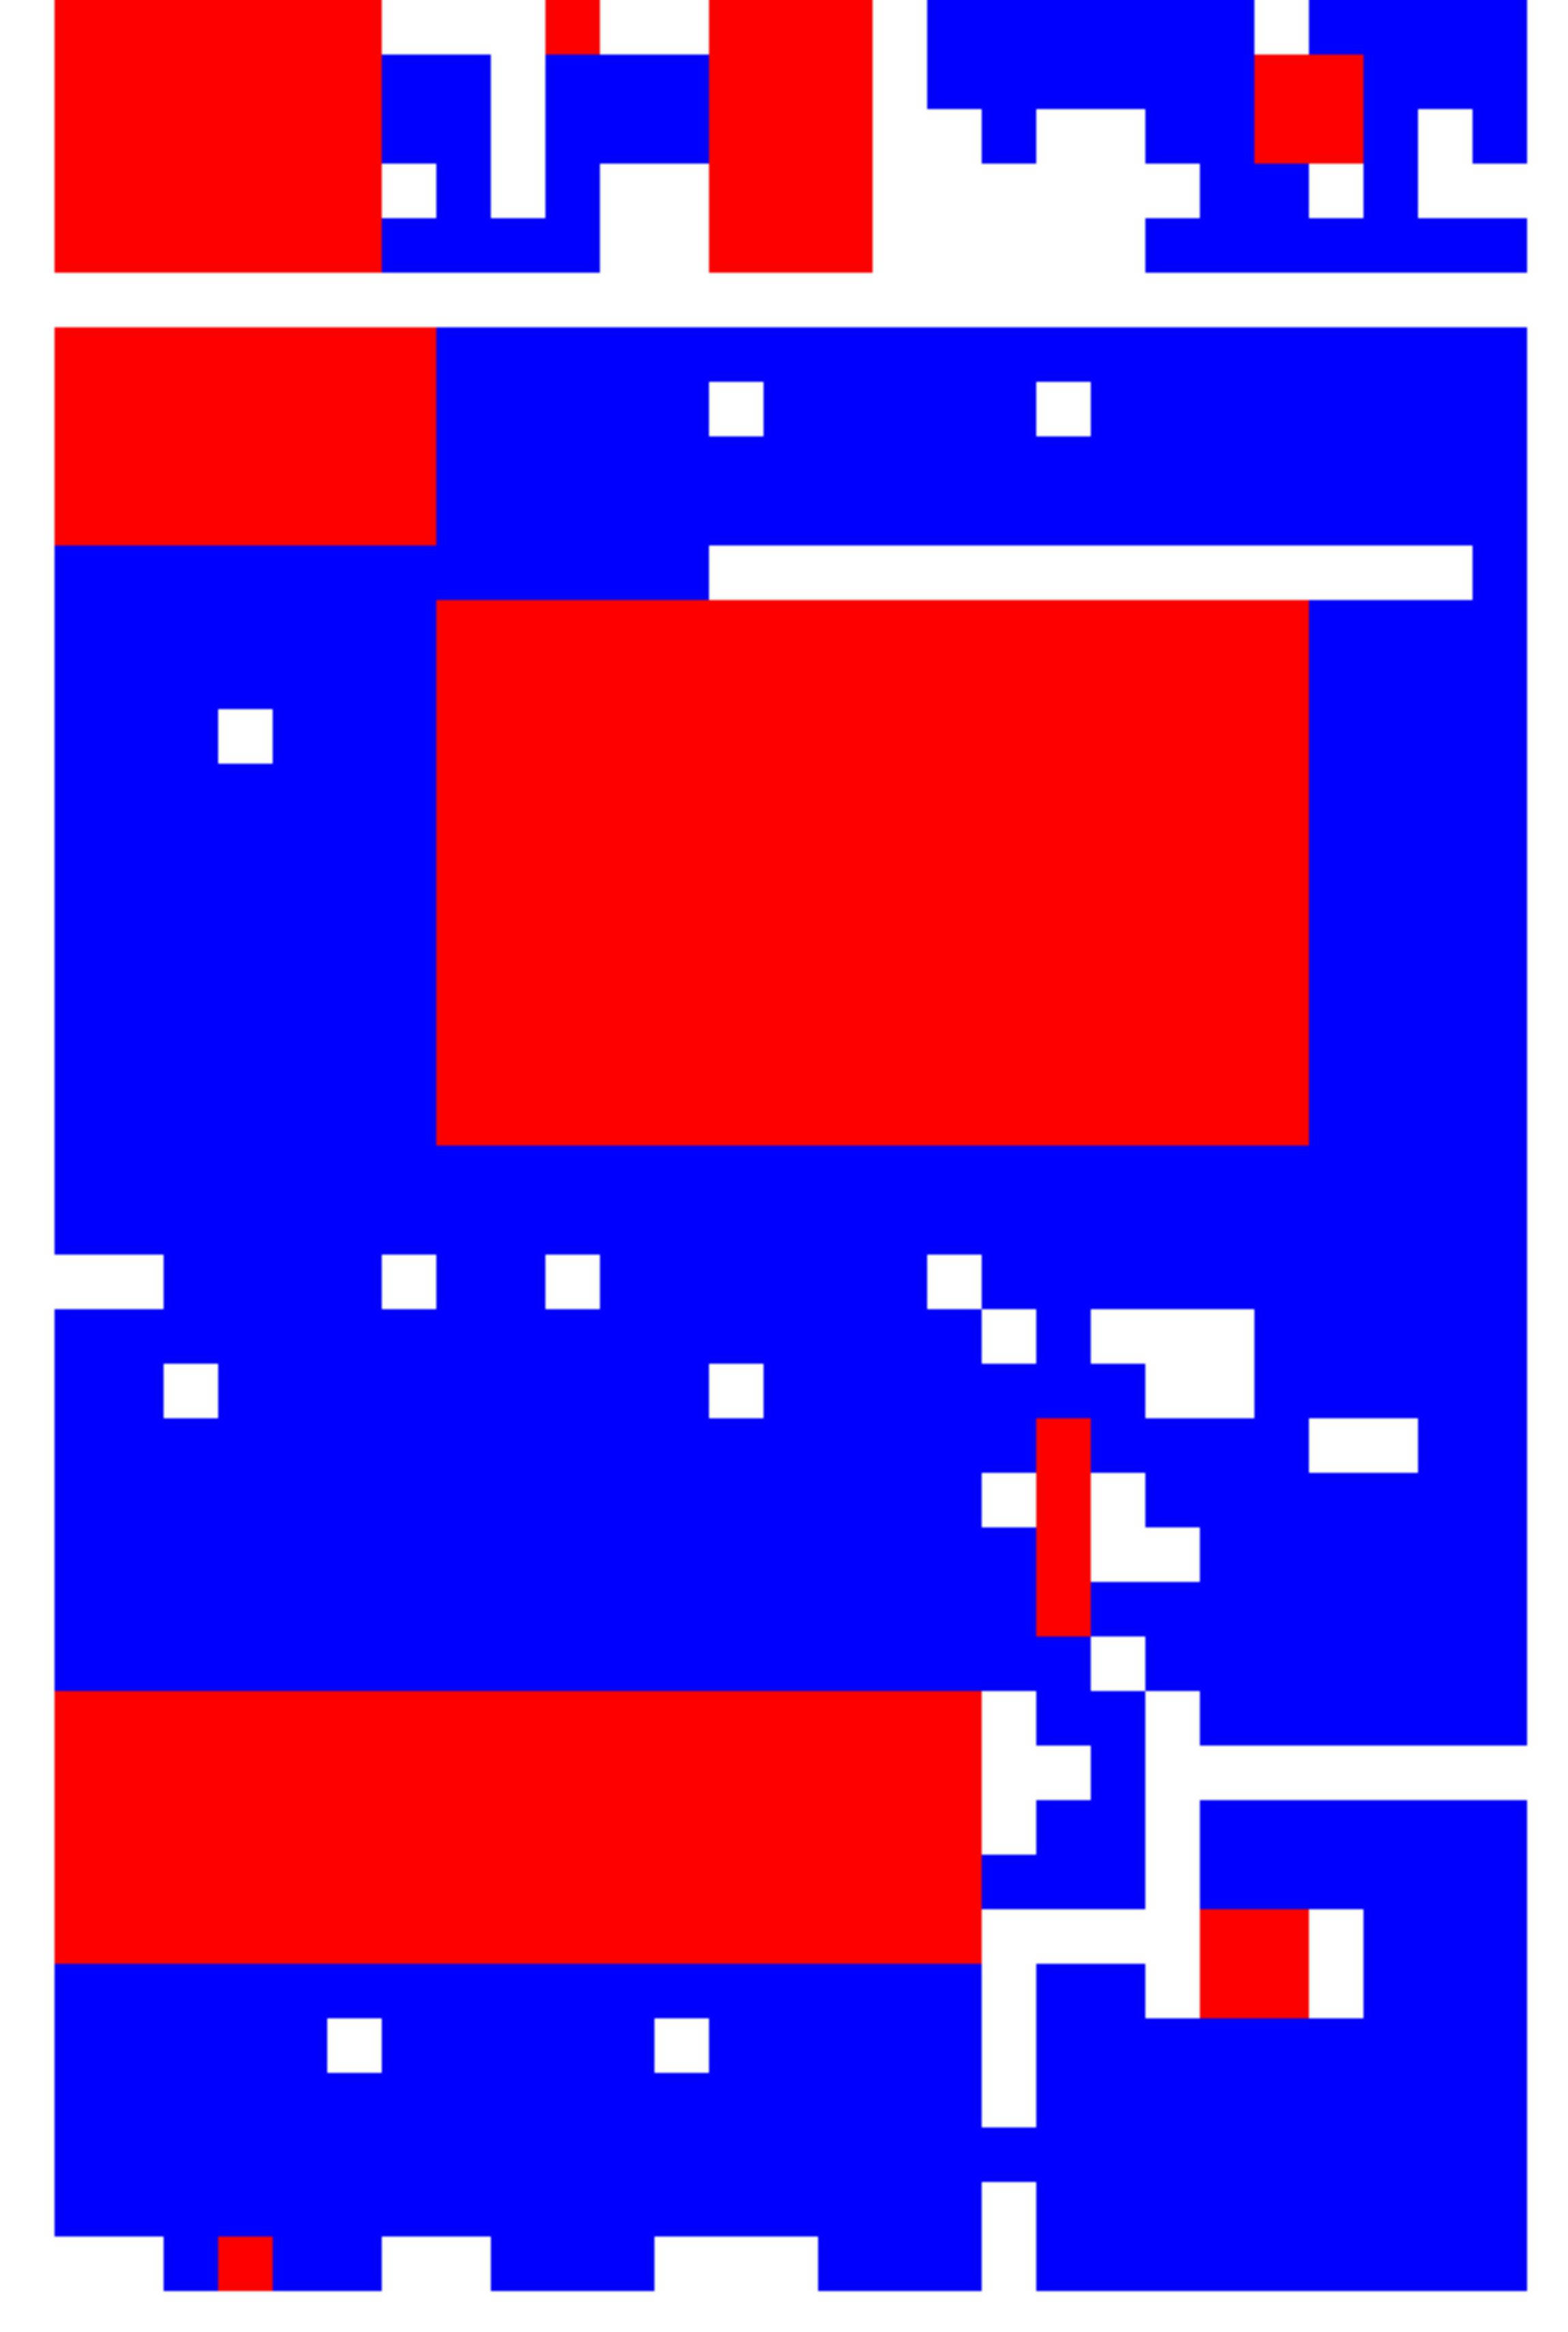
\includegraphics[scale=0.05]{../test/hebraic_res_hog_hsv_kmeans.jpg}
\end{center}
\caption{test de la méthode sur l'image hebraic.jpg}
\label{test2}
\end{figure}

\begin{figure}[H]
\begin{center}
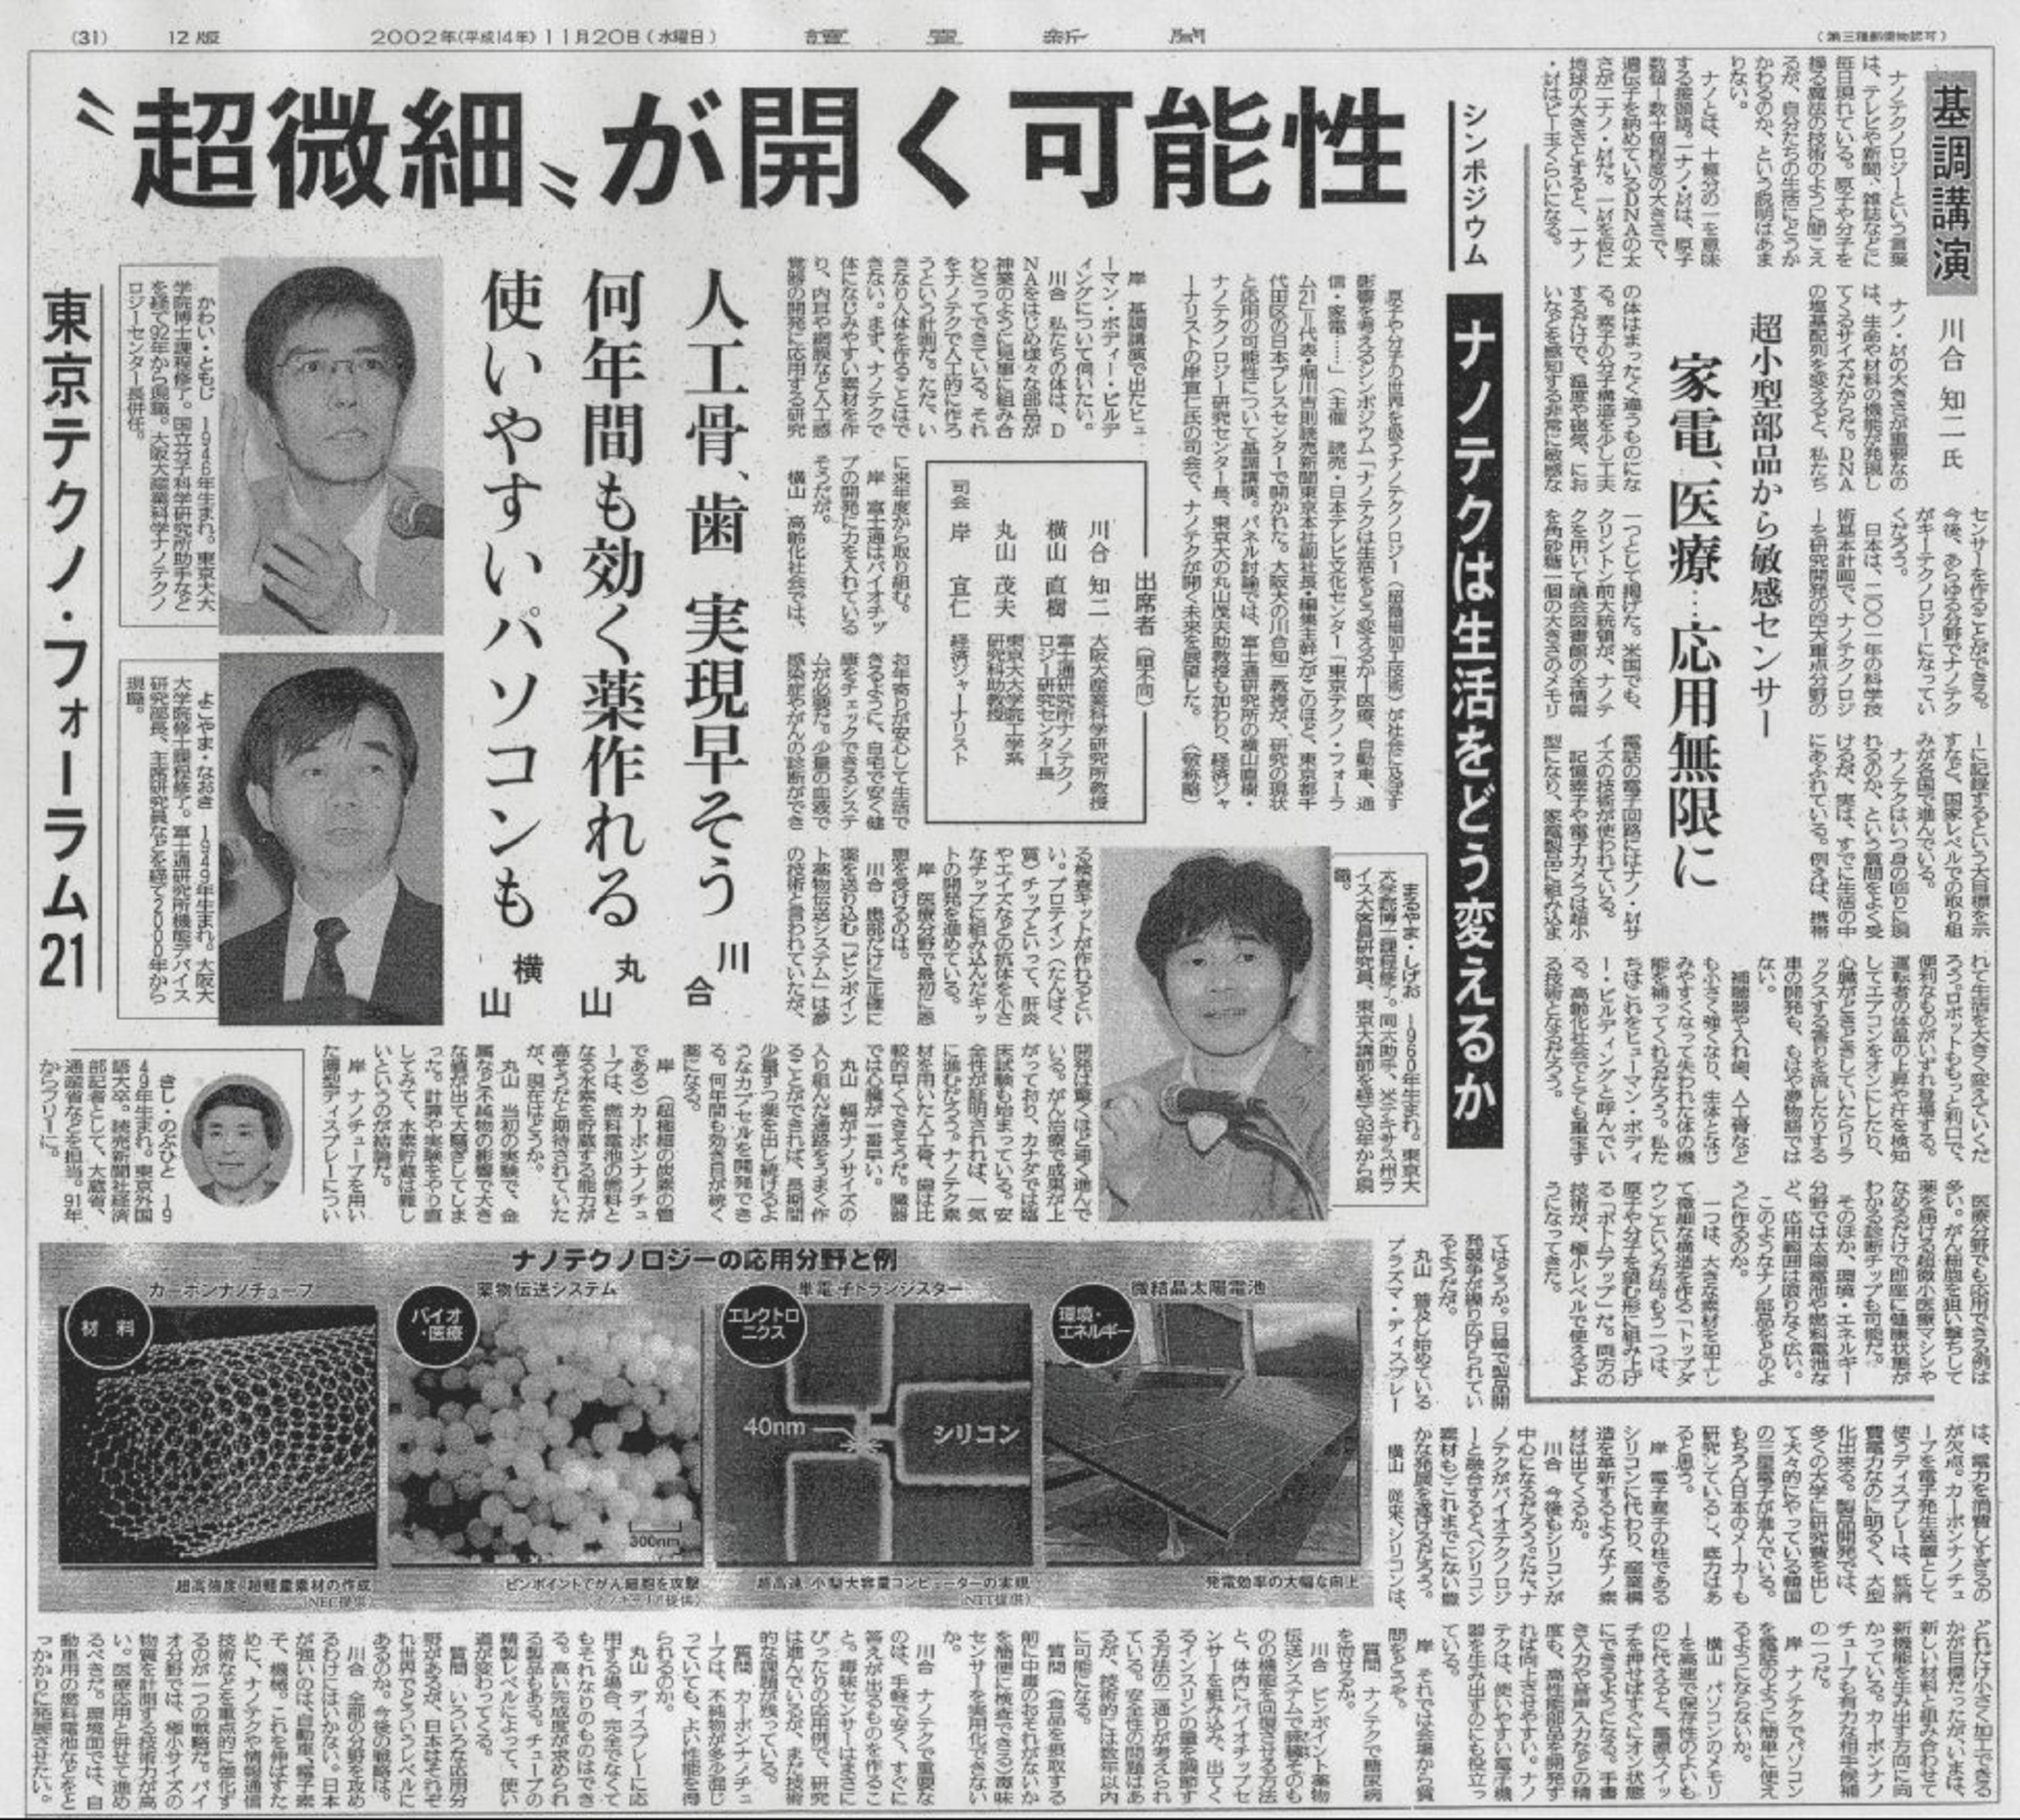
\includegraphics[scale=0.05]{../test/japanese.jpg}
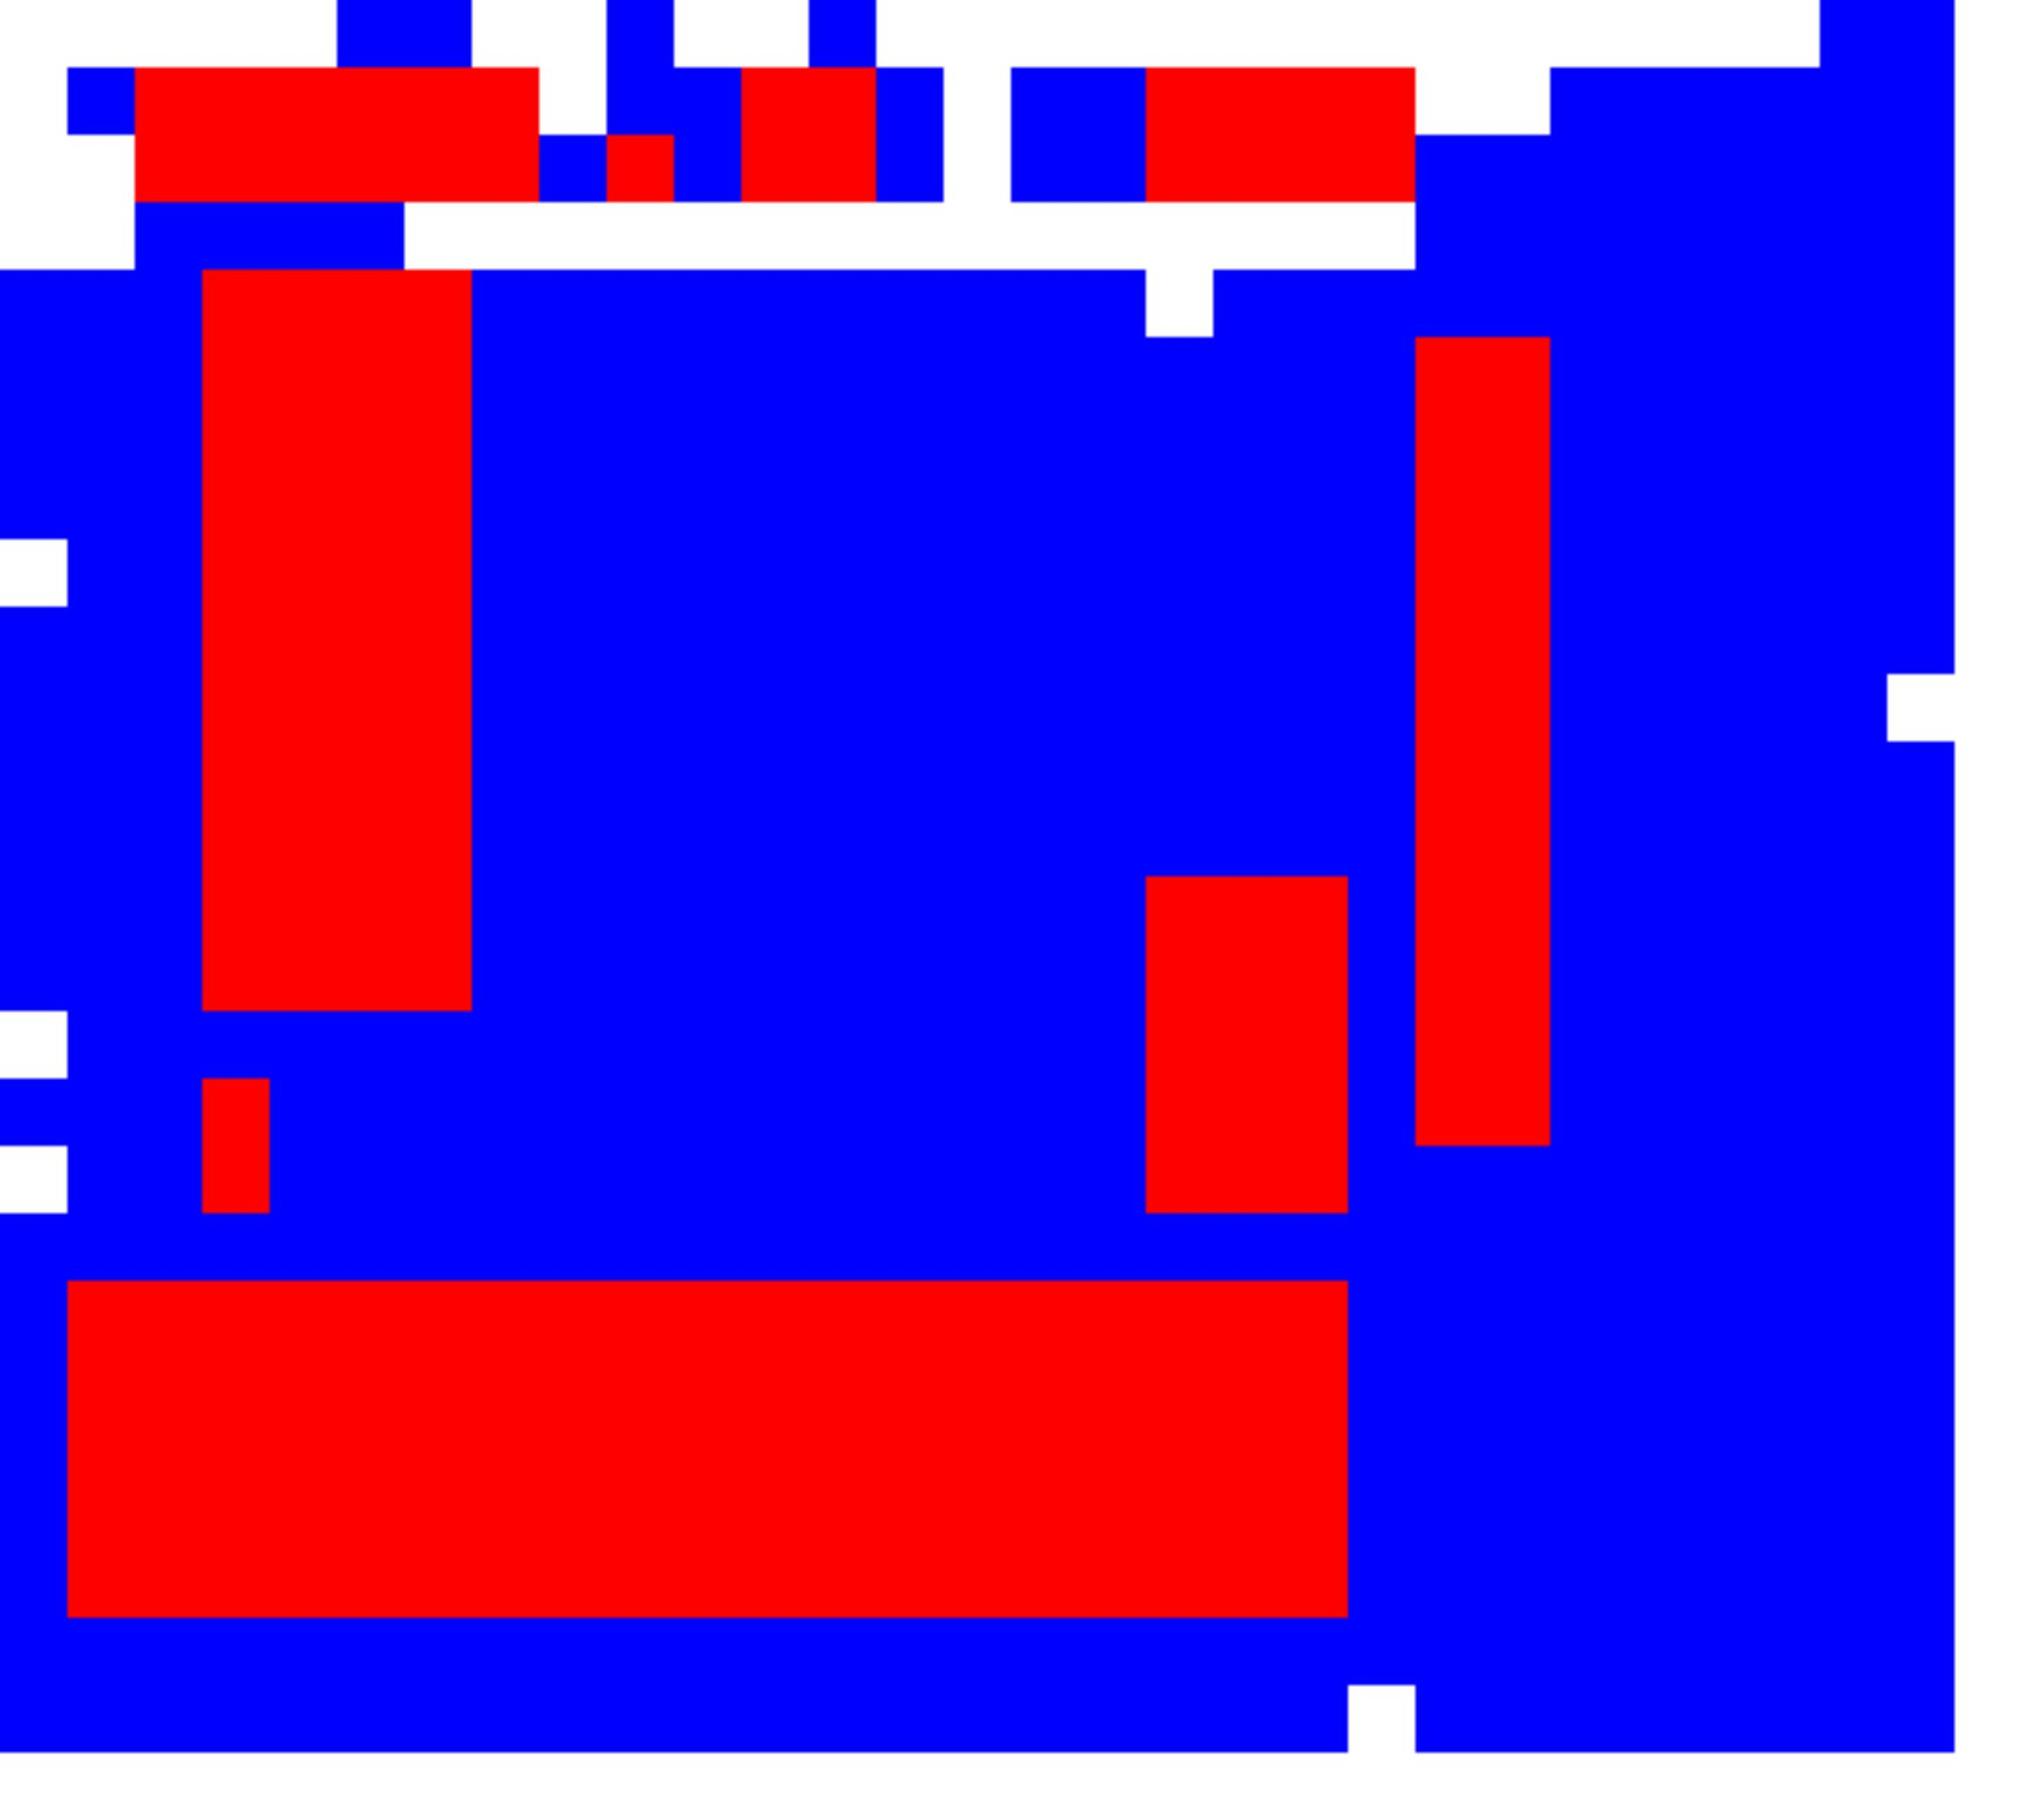
\includegraphics[scale=0.05]{../test/japanese_res_hog_hsv_kmeans.jpg}
\end{center}
\caption{test de la méthode sur l'image japanese.jpg}
\label{test3}
\end{figure}

\chapter{Code}

Le code $Python$ ayant permis les calculs présentés, se constitue de trois fichiers :
\begin{description} % listes descriptives

\item[$utils.py$ :] Ce fichier contient les fonctions pour le découpage de l'image en patch.
\item[$functions.py$ :] Ce fichier contient les fonctions permettant l'extraction des features. Ces fonctions utilisent $OpenCV$ \cite{opencv_library} ainsi que $scikit-learn$ \cite{scikit-learn}
\item[$run.py$ :] Ce fichier est le fichier principal. Il télécharge le dataset, le decompresse et lance le processus de clusterisation. Il affiche aussi les performances
en précision/rappel à partir des images de vérité terrain. Il contient aussi les différents paramètres comme la taille de voisinage, la nature des descripteurs...

\end{description}


\chapter{Resultats}

Parmi le dataset de 101 fichiers, certains au nombre de 5 ne presentent pas réellement de fond blanc, ce qui fausse l'étape de seuillage qui elle suppose l'existence d'une telle
propriété.\\
Nous présentons donc ci-après les résultats sur 96 fichiers avec les descripteurs $HOG+HSV$ décomposés par $KMeans$ :\\

\begin{figure}[H]
\begin{center}
\includegraphics[scale=0.6]{../data_papers/10_res_hog_hsv_kmeans_all.jpg}
\end{center}
\caption{de gauche à droite : image 10.jpg, binarisation, decomposition, vérité-terrain}
\label{10}
\end{figure}
\clearpage


\begin{figure}[H]
\begin{center}
\includegraphics[scale=0.6]{../data_papers/11_res_hog_hsv_kmeans_all.jpg}
\end{center}
\caption{de gauche à droite : image 11.jpg, binarisation, decomposition, vérité-terrain}
\label{11}
\end{figure}
\clearpage


\begin{figure}[H]
\begin{center}
\includegraphics[scale=0.6]{../data_papers/12_res_hog_hsv_kmeans_all.jpg}
\end{center}
\caption{de gauche à droite : image 12.jpg, binarisation, decomposition, vérité-terrain}
\label{12}
\end{figure}
\clearpage


\begin{figure}[H]
\begin{center}
\includegraphics[scale=0.6]{../data_papers/13_res_hog_hsv_kmeans_all.jpg}
\end{center}
\caption{de gauche à droite : image 13.jpg, binarisation, decomposition, vérité-terrain}
\label{13}
\end{figure}
\clearpage


\begin{figure}[H]
\begin{center}
\includegraphics[scale=0.6]{../data_papers/14_res_hog_hsv_kmeans_all.jpg}
\end{center}
\caption{de gauche à droite : image 14.jpg, binarisation, decomposition, vérité-terrain}
\label{14}
\end{figure}
\clearpage


\begin{figure}[H]
\begin{center}
\includegraphics[scale=0.6]{../data_papers/15_res_hog_hsv_kmeans_all.jpg}
\end{center}
\caption{de gauche à droite : image 15.jpg, binarisation, decomposition, vérité-terrain}
\label{15}
\end{figure}
\clearpage


\begin{figure}[H]
\begin{center}
\includegraphics[scale=0.6]{../data_papers/16_res_hog_hsv_kmeans_all.jpg}
\end{center}
\caption{de gauche à droite : image 16.jpg, binarisation, decomposition, vérité-terrain}
\label{16}
\end{figure}
\clearpage


\begin{figure}[H]
\begin{center}
\includegraphics[scale=0.6]{../data_papers/17_res_hog_hsv_kmeans_all.jpg}
\end{center}
\caption{de gauche à droite : image 17.jpg, binarisation, decomposition, vérité-terrain}
\label{17}
\end{figure}
\clearpage


\begin{figure}[H]
\begin{center}
\includegraphics[scale=0.6]{../data_papers/18_res_hog_hsv_kmeans_all.jpg}
\end{center}
\caption{de gauche à droite : image 18.jpg, binarisation, decomposition, vérité-terrain}
\label{18}
\end{figure}
\clearpage


\begin{figure}[H]
\begin{center}
\includegraphics[scale=0.6]{../data_papers/19_res_hog_hsv_kmeans_all.jpg}
\end{center}
\caption{de gauche à droite : image 19.jpg, binarisation, decomposition, vérité-terrain}
\label{19}
\end{figure}
\clearpage


\begin{figure}[H]
\begin{center}
\includegraphics[scale=0.6]{../data_papers/1cw_res_hog_hsv_kmeans_all.jpg}
\end{center}
\caption{de gauche à droite : image 1cw.bmp, binarisation, decomposition, vérité-terrain}
\label{1cw}
\end{figure}
\clearpage


\begin{figure}[H]
\begin{center}
\includegraphics[scale=0.6]{../data_papers/1g_res_hog_hsv_kmeans_all.jpg}
\end{center}
\caption{de gauche à droite : image 1g.tif, binarisation, decomposition, vérité-terrain}
\label{1g}
\end{figure}
\clearpage


\begin{figure}[H]
\begin{center}
\includegraphics[scale=0.6]{../data_papers/1_res_hog_hsv_kmeans_all.jpg}
\end{center}
\caption{de gauche à droite : image 1.jpg, binarisation, decomposition, vérité-terrain}
\label{1}
\end{figure}
\clearpage


\begin{figure}[H]
\begin{center}
\includegraphics[scale=0.6]{../data_papers/1m_res_hog_hsv_kmeans_all.jpg}
\end{center}
\caption{de gauche à droite : image 1m.bmp, binarisation, decomposition, vérité-terrain}
\label{1m}
\end{figure}
\clearpage


\begin{figure}[H]
\begin{center}
\includegraphics[scale=0.6]{../data_papers/1s_res_hog_hsv_kmeans_all.jpg}
\end{center}
\caption{de gauche à droite : image 1s.bmp, binarisation, decomposition, vérité-terrain}
\label{1s}
\end{figure}
\clearpage


\begin{figure}[H]
\begin{center}
\includegraphics[scale=0.6]{../data_papers/20_res_hog_hsv_kmeans_all.jpg}
\end{center}
\caption{de gauche à droite : image 20.jpg, binarisation, decomposition, vérité-terrain}
\label{20}
\end{figure}
\clearpage


\begin{figure}[H]
\begin{center}
\includegraphics[scale=0.6]{../data_papers/21_res_hog_hsv_kmeans_all.jpg}
\end{center}
\caption{de gauche à droite : image 21.jpg, binarisation, decomposition, vérité-terrain}
\label{21}
\end{figure}
\clearpage


\begin{figure}[H]
\begin{center}
\includegraphics[scale=0.6]{../data_papers/22_res_hog_hsv_kmeans_all.jpg}
\end{center}
\caption{de gauche à droite : image 22.jpg, binarisation, decomposition, vérité-terrain}
\label{22}
\end{figure}
\clearpage


\begin{figure}[H]
\begin{center}
\includegraphics[scale=0.6]{../data_papers/23_res_hog_hsv_kmeans_all.jpg}
\end{center}
\caption{de gauche à droite : image 23.jpg, binarisation, decomposition, vérité-terrain}
\label{23}
\end{figure}
\clearpage


\begin{figure}[H]
\begin{center}
\includegraphics[scale=0.6]{../data_papers/24_res_hog_hsv_kmeans_all.jpg}
\end{center}
\caption{de gauche à droite : image 24.jpg, binarisation, decomposition, vérité-terrain}
\label{24}
\end{figure}
\clearpage


\begin{figure}[H]
\begin{center}
\includegraphics[scale=0.6]{../data_papers/25_res_hog_hsv_kmeans_all.jpg}
\end{center}
\caption{de gauche à droite : image 25.jpg, binarisation, decomposition, vérité-terrain}
\label{25}
\end{figure}
\clearpage


\begin{figure}[H]
\begin{center}
\includegraphics[scale=0.6]{../data_papers/26_res_hog_hsv_kmeans_all.jpg}
\end{center}
\caption{de gauche à droite : image 26.jpg, binarisation, decomposition, vérité-terrain}
\label{26}
\end{figure}
\clearpage


\begin{figure}[H]
\begin{center}
\includegraphics[scale=0.6]{../data_papers/27_res_hog_hsv_kmeans_all.jpg}
\end{center}
\caption{de gauche à droite : image 27.jpg, binarisation, decomposition, vérité-terrain}
\label{27}
\end{figure}
\clearpage


\begin{figure}[H]
\begin{center}
\includegraphics[scale=0.6]{../data_papers/28_res_hog_hsv_kmeans_all.jpg}
\end{center}
\caption{de gauche à droite : image 28.jpg, binarisation, decomposition, vérité-terrain}
\label{28}
\end{figure}
\clearpage


\begin{figure}[H]
\begin{center}
\includegraphics[scale=0.6]{../data_papers/29_res_hog_hsv_kmeans_all.jpg}
\end{center}
\caption{de gauche à droite : image 29.jpg, binarisation, decomposition, vérité-terrain}
\label{29}
\end{figure}
\clearpage


\begin{figure}[H]
\begin{center}
\includegraphics[scale=0.6]{../data_papers/2cw_res_hog_hsv_kmeans_all.jpg}
\end{center}
\caption{de gauche à droite : image 2cw.bmp, binarisation, decomposition, vérité-terrain}
\label{2cw}
\end{figure}
\clearpage


\begin{figure}[H]
\begin{center}
\includegraphics[scale=0.6]{../data_papers/2g_res_hog_hsv_kmeans_all.jpg}
\end{center}
\caption{de gauche à droite : image 2g.tif, binarisation, decomposition, vérité-terrain}
\label{2g}
\end{figure}
\clearpage


\begin{figure}[H]
\begin{center}
\includegraphics[scale=0.6]{../data_papers/2_res_hog_hsv_kmeans_all.jpg}
\end{center}
\caption{de gauche à droite : image 2.jpg, binarisation, decomposition, vérité-terrain}
\label{2}
\end{figure}
\clearpage


\begin{figure}[H]
\begin{center}
\includegraphics[scale=0.6]{../data_papers/2m_res_hog_hsv_kmeans_all.jpg}
\end{center}
\caption{de gauche à droite : image 2m.bmp, binarisation, decomposition, vérité-terrain}
\label{2m}
\end{figure}
\clearpage


\begin{figure}[H]
\begin{center}
\includegraphics[scale=0.6]{../data_papers/2s_res_hog_hsv_kmeans_all.jpg}
\end{center}
\caption{de gauche à droite : image 2s.bmp, binarisation, decomposition, vérité-terrain}
\label{2s}
\end{figure}
\clearpage


\begin{figure}[H]
\begin{center}
\includegraphics[scale=0.6]{../data_papers/30_res_hog_hsv_kmeans_all.jpg}
\end{center}
\caption{de gauche à droite : image 30.jpg, binarisation, decomposition, vérité-terrain}
\label{30}
\end{figure}
\clearpage


\begin{figure}[H]
\begin{center}
\includegraphics[scale=0.6]{../data_papers/31_res_hog_hsv_kmeans_all.jpg}
\end{center}
\caption{de gauche à droite : image 31.jpg, binarisation, decomposition, vérité-terrain}
\label{31}
\end{figure}
\clearpage


\begin{figure}[H]
\begin{center}
\includegraphics[scale=0.6]{../data_papers/32_res_hog_hsv_kmeans_all.jpg}
\end{center}
\caption{de gauche à droite : image 32.jpg, binarisation, decomposition, vérité-terrain}
\label{32}
\end{figure}
\clearpage


\begin{figure}[H]
\begin{center}
\includegraphics[scale=0.6]{../data_papers/33_res_hog_hsv_kmeans_all.jpg}
\end{center}
\caption{de gauche à droite : image 33.jpg, binarisation, decomposition, vérité-terrain}
\label{33}
\end{figure}
\clearpage


\begin{figure}[H]
\begin{center}
\includegraphics[scale=0.6]{../data_papers/34_res_hog_hsv_kmeans_all.jpg}
\end{center}
\caption{de gauche à droite : image 34.jpg, binarisation, decomposition, vérité-terrain}
\label{34}
\end{figure}
\clearpage


\begin{figure}[H]
\begin{center}
\includegraphics[scale=0.6]{../data_papers/35_res_hog_hsv_kmeans_all.jpg}
\end{center}
\caption{de gauche à droite : image 35.jpg, binarisation, decomposition, vérité-terrain}
\label{35}
\end{figure}
\clearpage


\begin{figure}[H]
\begin{center}
\includegraphics[scale=0.6]{../data_papers/36_res_hog_hsv_kmeans_all.jpg}
\end{center}
\caption{de gauche à droite : image 36.jpg, binarisation, decomposition, vérité-terrain}
\label{36}
\end{figure}
\clearpage


\begin{figure}[H]
\begin{center}
\includegraphics[scale=0.6]{../data_papers/37_res_hog_hsv_kmeans_all.jpg}
\end{center}
\caption{de gauche à droite : image 37.jpg, binarisation, decomposition, vérité-terrain}
\label{37}
\end{figure}
\clearpage


\begin{figure}[H]
\begin{center}
\includegraphics[scale=0.6]{../data_papers/38_res_hog_hsv_kmeans_all.jpg}
\end{center}
\caption{de gauche à droite : image 38.jpg, binarisation, decomposition, vérité-terrain}
\label{38}
\end{figure}
\clearpage


\begin{figure}[H]
\begin{center}
\includegraphics[scale=0.6]{../data_papers/39_res_hog_hsv_kmeans_all.jpg}
\end{center}
\caption{de gauche à droite : image 39.jpg, binarisation, decomposition, vérité-terrain}
\label{39}
\end{figure}
\clearpage


\begin{figure}[H]
\begin{center}
\includegraphics[scale=0.6]{../data_papers/3cw_res_hog_hsv_kmeans_all.jpg}
\end{center}
\caption{de gauche à droite : image 3cw.bmp, binarisation, decomposition, vérité-terrain}
\label{3cw}
\end{figure}
\clearpage


\begin{figure}[H]
\begin{center}
\includegraphics[scale=0.6]{../data_papers/3g_res_hog_hsv_kmeans_all.jpg}
\end{center}
\caption{de gauche à droite : image 3g.tif, binarisation, decomposition, vérité-terrain}
\label{3g}
\end{figure}
\clearpage


\begin{figure}[H]
\begin{center}
\includegraphics[scale=0.6]{../data_papers/3_res_hog_hsv_kmeans_all.jpg}
\end{center}
\caption{de gauche à droite : image 3.jpg, binarisation, decomposition, vérité-terrain}
\label{3}
\end{figure}
\clearpage


\begin{figure}[H]
\begin{center}
\includegraphics[scale=0.6]{../data_papers/3m_res_hog_hsv_kmeans_all.jpg}
\end{center}
\caption{de gauche à droite : image 3m.bmp, binarisation, decomposition, vérité-terrain}
\label{3m}
\end{figure}
\clearpage


\begin{figure}[H]
\begin{center}
\includegraphics[scale=0.6]{../data_papers/3s_res_hog_hsv_kmeans_all.jpg}
\end{center}
\caption{de gauche à droite : image 3s.bmp, binarisation, decomposition, vérité-terrain}
\label{3s}
\end{figure}
\clearpage


\begin{figure}[H]
\begin{center}
\includegraphics[scale=0.6]{../data_papers/40_res_hog_hsv_kmeans_all.jpg}
\end{center}
\caption{de gauche à droite : image 40.jpg, binarisation, decomposition, vérité-terrain}
\label{40}
\end{figure}
\clearpage


\begin{figure}[H]
\begin{center}
\includegraphics[scale=0.6]{../data_papers/41_res_hog_hsv_kmeans_all.jpg}
\end{center}
\caption{de gauche à droite : image 41.jpg, binarisation, decomposition, vérité-terrain}
\label{41}
\end{figure}
\clearpage


\begin{figure}[H]
\begin{center}
\includegraphics[scale=0.6]{../data_papers/42_res_hog_hsv_kmeans_all.jpg}
\end{center}
\caption{de gauche à droite : image 42.jpg, binarisation, decomposition, vérité-terrain}
\label{42}
\end{figure}
\clearpage


\begin{figure}[H]
\begin{center}
\includegraphics[scale=0.6]{../data_papers/43_res_hog_hsv_kmeans_all.jpg}
\end{center}
\caption{de gauche à droite : image 43.jpg, binarisation, decomposition, vérité-terrain}
\label{43}
\end{figure}
\clearpage


\begin{figure}[H]
\begin{center}
\includegraphics[scale=0.6]{../data_papers/44_res_hog_hsv_kmeans_all.jpg}
\end{center}
\caption{de gauche à droite : image 44.jpg, binarisation, decomposition, vérité-terrain}
\label{44}
\end{figure}
\clearpage


\begin{figure}[H]
\begin{center}
\includegraphics[scale=0.6]{../data_papers/45_res_hog_hsv_kmeans_all.jpg}
\end{center}
\caption{de gauche à droite : image 45.jpg, binarisation, decomposition, vérité-terrain}
\label{45}
\end{figure}
\clearpage


\begin{figure}[H]
\begin{center}
\includegraphics[scale=0.6]{../data_papers/46_res_hog_hsv_kmeans_all.jpg}
\end{center}
\caption{de gauche à droite : image 46.jpg, binarisation, decomposition, vérité-terrain}
\label{46}
\end{figure}
\clearpage


\begin{figure}[H]
\begin{center}
\includegraphics[scale=0.6]{../data_papers/47_res_hog_hsv_kmeans_all.jpg}
\end{center}
\caption{de gauche à droite : image 47.jpg, binarisation, decomposition, vérité-terrain}
\label{47}
\end{figure}
\clearpage


\begin{figure}[H]
\begin{center}
\includegraphics[scale=0.6]{../data_papers/48_res_hog_hsv_kmeans_all.jpg}
\end{center}
\caption{de gauche à droite : image 48.jpg, binarisation, decomposition, vérité-terrain}
\label{48}
\end{figure}
\clearpage


\begin{figure}[H]
\begin{center}
\includegraphics[scale=0.6]{../data_papers/49_res_hog_hsv_kmeans_all.jpg}
\end{center}
\caption{de gauche à droite : image 49.jpg, binarisation, decomposition, vérité-terrain}
\label{49}
\end{figure}
\clearpage


\begin{figure}[H]
\begin{center}
\includegraphics[scale=0.6]{../data_papers/4cw_res_hog_hsv_kmeans_all.jpg}
\end{center}
\caption{de gauche à droite : image 4cw.bmp, binarisation, decomposition, vérité-terrain}
\label{4cw}
\end{figure}
\clearpage


\begin{figure}[H]
\begin{center}
\includegraphics[scale=0.6]{../data_papers/4g_res_hog_hsv_kmeans_all.jpg}
\end{center}
\caption{de gauche à droite : image 4g.tif, binarisation, decomposition, vérité-terrain}
\label{4g}
\end{figure}
\clearpage


\begin{figure}[H]
\begin{center}
\includegraphics[scale=0.6]{../data_papers/4_res_hog_hsv_kmeans_all.jpg}
\end{center}
\caption{de gauche à droite : image 4.jpg, binarisation, decomposition, vérité-terrain}
\label{4}
\end{figure}
\clearpage


\begin{figure}[H]
\begin{center}
\includegraphics[scale=0.6]{../data_papers/4m_res_hog_hsv_kmeans_all.jpg}
\end{center}
\caption{de gauche à droite : image 4m.bmp, binarisation, decomposition, vérité-terrain}
\label{4m}
\end{figure}
\clearpage


\begin{figure}[H]
\begin{center}
\includegraphics[scale=0.6]{../data_papers/4s_res_hog_hsv_kmeans_all.jpg}
\end{center}
\caption{de gauche à droite : image 4s.bmp, binarisation, decomposition, vérité-terrain}
\label{4s}
\end{figure}
\clearpage


\begin{figure}[H]
\begin{center}
\includegraphics[scale=0.6]{../data_papers/50_res_hog_hsv_kmeans_all.jpg}
\end{center}
\caption{de gauche à droite : image 50.jpg, binarisation, decomposition, vérité-terrain}
\label{50}
\end{figure}
\clearpage


\begin{figure}[H]
\begin{center}
\includegraphics[scale=0.6]{../data_papers/51_res_hog_hsv_kmeans_all.jpg}
\end{center}
\caption{de gauche à droite : image 51.jpg, binarisation, decomposition, vérité-terrain}
\label{51}
\end{figure}
\clearpage


\begin{figure}[H]
\begin{center}
\includegraphics[scale=0.6]{../data_papers/52_res_hog_hsv_kmeans_all.jpg}
\end{center}
\caption{de gauche à droite : image 52.jpg, binarisation, decomposition, vérité-terrain}
\label{52}
\end{figure}
\clearpage


\begin{figure}[H]
\begin{center}
\includegraphics[scale=0.6]{../data_papers/53_res_hog_hsv_kmeans_all.jpg}
\end{center}
\caption{de gauche à droite : image 53.jpg, binarisation, decomposition, vérité-terrain}
\label{53}
\end{figure}
\clearpage


\begin{figure}[H]
\begin{center}
\includegraphics[scale=0.6]{../data_papers/54_res_hog_hsv_kmeans_all.jpg}
\end{center}
\caption{de gauche à droite : image 54.jpg, binarisation, decomposition, vérité-terrain}
\label{54}
\end{figure}
\clearpage


\begin{figure}[H]
\begin{center}
\includegraphics[scale=0.6]{../data_papers/55_res_hog_hsv_kmeans_all.jpg}
\end{center}
\caption{de gauche à droite : image 55.jpg, binarisation, decomposition, vérité-terrain}
\label{55}
\end{figure}
\clearpage


\begin{figure}[H]
\begin{center}
\includegraphics[scale=0.6]{../data_papers/56_res_hog_hsv_kmeans_all.jpg}
\end{center}
\caption{de gauche à droite : image 56.jpg, binarisation, decomposition, vérité-terrain}
\label{56}
\end{figure}
\clearpage


\begin{figure}[H]
\begin{center}
\includegraphics[scale=0.6]{../data_papers/57_res_hog_hsv_kmeans_all.jpg}
\end{center}
\caption{de gauche à droite : image 57.jpg, binarisation, decomposition, vérité-terrain}
\label{57}
\end{figure}
\clearpage


\begin{figure}[H]
\begin{center}
\includegraphics[scale=0.6]{../data_papers/58_res_hog_hsv_kmeans_all.jpg}
\end{center}
\caption{de gauche à droite : image 58.jpg, binarisation, decomposition, vérité-terrain}
\label{58}
\end{figure}
\clearpage


\begin{figure}[H]
\begin{center}
\includegraphics[scale=0.6]{../data_papers/59_res_hog_hsv_kmeans_all.jpg}
\end{center}
\caption{de gauche à droite : image 59.jpg, binarisation, decomposition, vérité-terrain}
\label{59}
\end{figure}
\clearpage


\begin{figure}[H]
\begin{center}
\includegraphics[scale=0.6]{../data_papers/5cw_res_hog_hsv_kmeans_all.jpg}
\end{center}
\caption{de gauche à droite : image 5cw.bmp, binarisation, decomposition, vérité-terrain}
\label{5cw}
\end{figure}
\clearpage


\begin{figure}[H]
\begin{center}
\includegraphics[scale=0.6]{../data_papers/5g_res_hog_hsv_kmeans_all.jpg}
\end{center}
\caption{de gauche à droite : image 5g.tif, binarisation, decomposition, vérité-terrain}
\label{5g}
\end{figure}
\clearpage


\begin{figure}[H]
\begin{center}
\includegraphics[scale=0.6]{../data_papers/5_res_hog_hsv_kmeans_all.jpg}
\end{center}
\caption{de gauche à droite : image 5.jpg, binarisation, decomposition, vérité-terrain}
\label{5}
\end{figure}
\clearpage


\begin{figure}[H]
\begin{center}
\includegraphics[scale=0.6]{../data_papers/5m_res_hog_hsv_kmeans_all.jpg}
\end{center}
\caption{de gauche à droite : image 5m.bmp, binarisation, decomposition, vérité-terrain}
\label{5m}
\end{figure}
\clearpage


\begin{figure}[H]
\begin{center}
\includegraphics[scale=0.6]{../data_papers/5s_res_hog_hsv_kmeans_all.jpg}
\end{center}
\caption{de gauche à droite : image 5s.bmp, binarisation, decomposition, vérité-terrain}
\label{5s}
\end{figure}
\clearpage


\begin{figure}[H]
\begin{center}
\includegraphics[scale=0.6]{../data_papers/60_res_hog_hsv_kmeans_all.jpg}
\end{center}
\caption{de gauche à droite : image 60.jpg, binarisation, decomposition, vérité-terrain}
\label{60}
\end{figure}
\clearpage


\begin{figure}[H]
\begin{center}
\includegraphics[scale=0.6]{../data_papers/61_res_hog_hsv_kmeans_all.jpg}
\end{center}
\caption{de gauche à droite : image 61.jpg, binarisation, decomposition, vérité-terrain}
\label{61}
\end{figure}
\clearpage


\begin{figure}[H]
\begin{center}
\includegraphics[scale=0.6]{../data_papers/62_res_hog_hsv_kmeans_all.jpg}
\end{center}
\caption{de gauche à droite : image 62.jpg, binarisation, decomposition, vérité-terrain}
\label{62}
\end{figure}
\clearpage


\begin{figure}[H]
\begin{center}
\includegraphics[scale=0.6]{../data_papers/63_res_hog_hsv_kmeans_all.jpg}
\end{center}
\caption{de gauche à droite : image 63.jpg, binarisation, decomposition, vérité-terrain}
\label{63}
\end{figure}
\clearpage


\begin{figure}[H]
\begin{center}
\includegraphics[scale=0.6]{../data_papers/64_res_hog_hsv_kmeans_all.jpg}
\end{center}
\caption{de gauche à droite : image 64.jpg, binarisation, decomposition, vérité-terrain}
\label{64}
\end{figure}
\clearpage


\begin{figure}[H]
\begin{center}
\includegraphics[scale=0.6]{../data_papers/65_res_hog_hsv_kmeans_all.jpg}
\end{center}
\caption{de gauche à droite : image 65.jpg, binarisation, decomposition, vérité-terrain}
\label{65}
\end{figure}
\clearpage


\begin{figure}[H]
\begin{center}
\includegraphics[scale=0.6]{../data_papers/66_res_hog_hsv_kmeans_all.jpg}
\end{center}
\caption{de gauche à droite : image 66.jpg, binarisation, decomposition, vérité-terrain}
\label{66}
\end{figure}
\clearpage


\begin{figure}[H]
\begin{center}
\includegraphics[scale=0.6]{../data_papers/67_res_hog_hsv_kmeans_all.jpg}
\end{center}
\caption{de gauche à droite : image 67.jpg, binarisation, decomposition, vérité-terrain}
\label{67}
\end{figure}
\clearpage


\begin{figure}[H]
\begin{center}
\includegraphics[scale=0.6]{../data_papers/68_res_hog_hsv_kmeans_all.jpg}
\end{center}
\caption{de gauche à droite : image 68.jpg, binarisation, decomposition, vérité-terrain}
\label{68}
\end{figure}
\clearpage


\begin{figure}[H]
\begin{center}
\includegraphics[scale=0.6]{../data_papers/69_res_hog_hsv_kmeans_all.jpg}
\end{center}
\caption{de gauche à droite : image 69.jpg, binarisation, decomposition, vérité-terrain}
\label{69}
\end{figure}
\clearpage


\begin{figure}[H]
\begin{center}
\includegraphics[scale=0.6]{../data_papers/6cw_res_hog_hsv_kmeans_all.jpg}
\end{center}
\caption{de gauche à droite : image 6cw.bmp, binarisation, decomposition, vérité-terrain}
\label{6cw}
\end{figure}
\clearpage


\begin{figure}[H]
\begin{center}
\includegraphics[scale=0.6]{../data_papers/6g_res_hog_hsv_kmeans_all.jpg}
\end{center}
\caption{de gauche à droite : image 6g.tif, binarisation, decomposition, vérité-terrain}
\label{6g}
\end{figure}
\clearpage


\begin{figure}[H]
\begin{center}
\includegraphics[scale=0.6]{../data_papers/6_res_hog_hsv_kmeans_all.jpg}
\end{center}
\caption{de gauche à droite : image 6.jpg, binarisation, decomposition, vérité-terrain}
\label{6}
\end{figure}
\clearpage


\begin{figure}[H]
\begin{center}
\includegraphics[scale=0.6]{../data_papers/6m_res_hog_hsv_kmeans_all.jpg}
\end{center}
\caption{de gauche à droite : image 6m.bmp, binarisation, decomposition, vérité-terrain}
\label{6m}
\end{figure}
\clearpage


\begin{figure}[H]
\begin{center}
\includegraphics[scale=0.6]{../data_papers/6s_res_hog_hsv_kmeans_all.jpg}
\end{center}
\caption{de gauche à droite : image 6s.bmp, binarisation, decomposition, vérité-terrain}
\label{6s}
\end{figure}
\clearpage


\begin{figure}[H]
\begin{center}
\includegraphics[scale=0.6]{../data_papers/70_res_hog_hsv_kmeans_all.jpg}
\end{center}
\caption{de gauche à droite : image 70.jpg, binarisation, decomposition, vérité-terrain}
\label{70}
\end{figure}
\clearpage


\begin{figure}[H]
\begin{center}
\includegraphics[scale=0.6]{../data_papers/71_res_hog_hsv_kmeans_all.jpg}
\end{center}
\caption{de gauche à droite : image 71.jpg, binarisation, decomposition, vérité-terrain}
\label{71}
\end{figure}
\clearpage


\begin{figure}[H]
\begin{center}
\includegraphics[scale=0.6]{../data_papers/72_res_hog_hsv_kmeans_all.jpg}
\end{center}
\caption{de gauche à droite : image 72.jpg, binarisation, decomposition, vérité-terrain}
\label{72}
\end{figure}
\clearpage


\begin{figure}[H]
\begin{center}
\includegraphics[scale=0.6]{../data_papers/73_res_hog_hsv_kmeans_all.jpg}
\end{center}
\caption{de gauche à droite : image 73.jpg, binarisation, decomposition, vérité-terrain}
\label{73}
\end{figure}
\clearpage


\begin{figure}[H]
\begin{center}
\includegraphics[scale=0.6]{../data_papers/74_res_hog_hsv_kmeans_all.jpg}
\end{center}
\caption{de gauche à droite : image 74.jpg, binarisation, decomposition, vérité-terrain}
\label{74}
\end{figure}
\clearpage


\begin{figure}[H]
\begin{center}
\includegraphics[scale=0.6]{../data_papers/75_res_hog_hsv_kmeans_all.jpg}
\end{center}
\caption{de gauche à droite : image 75.jpg, binarisation, decomposition, vérité-terrain}
\label{75}
\end{figure}
\clearpage


\begin{figure}[H]
\begin{center}
\includegraphics[scale=0.6]{../data_papers/7_res_hog_hsv_kmeans_all.jpg}
\end{center}
\caption{de gauche à droite : image 7.jpg, binarisation, decomposition, vérité-terrain}
\label{7}
\end{figure}
\clearpage


\begin{figure}[H]
\begin{center}
\includegraphics[scale=0.6]{../data_papers/7m_res_hog_hsv_kmeans_all.jpg}
\end{center}
\caption{de gauche à droite : image 7m.tif, binarisation, decomposition, vérité-terrain}
\label{7m}
\end{figure}
\clearpage


\begin{figure}[H]
\begin{center}
\includegraphics[scale=0.6]{../data_papers/7s_res_hog_hsv_kmeans_all.jpg}
\end{center}
\caption{de gauche à droite : image 7s.bmp, binarisation, decomposition, vérité-terrain}
\label{7s}
\end{figure}
\clearpage


\begin{figure}[H]
\begin{center}
\includegraphics[scale=0.6]{../data_papers/8_res_hog_hsv_kmeans_all.jpg}
\end{center}
\caption{de gauche à droite : image 8.jpg, binarisation, decomposition, vérité-terrain}
\label{8}
\end{figure}
\clearpage


\begin{figure}[H]
\begin{center}
\includegraphics[scale=0.6]{../data_papers/9_res_hog_hsv_kmeans_all.jpg}
\end{center}
\caption{de gauche à droite : image 9.jpg, binarisation, decomposition, vérité-terrain}
\label{9}
\end{figure}
\clearpage


\clearpage

\backmatter

\listoftables

\listoffigures

\bibliographystyle{alpha}
\bibliography{biblio}

\end{document}